%% Customizacoes do abnTeX2 (http://abnTeX2.googlecode.com) para o IFRS Campus Osorio v1.1
%% Por Bruno Fernandes (bruno.fernandes@osorio.ifrs.edu.br)
%% O modelo mais atualizado está disponível em bit.ly/ADSLaTeX
%%
%% abtex2-modelo-trabalho-academico.tex, v-1.9.6 laurocesar
%% Copyright 2012-2016 by abnTeX2 group at http://www.abntex.net.br/ 
%%
%% This work may be distributed and/or modified under the
%% conditions of the LaTeX Project Public License, either version 1.3
%% of this license or (at your option) any later version.
%% The latest version of this license is in
%%   http://www.latex-project.org/lppl.txt
%% and version 1.3 or later is part of all distributions of LaTeX
%% version 2005/12/01 or later.
%%
%% This work has the LPPL maintenance status `maintained'.
%% 
%% The Current Maintainer of this work is the abnTeX2 team, led
%% by Lauro César Araujo. Further information are available on 
%% http://www.abntex.net.br/
%%
%% This work consists of the files abntex2-modelo-trabalho-academico.tex,
%% abntex2-modelo-include-comandos and abntex2-modelo-references.bib
%%

% ------------------------------------------------------------------------
% ------------------------------------------------------------------------
% abnTeX2: Modelo de Trabalho Academico (tese de doutorado, dissertacao de
% mestrado e trabalhos monos em geral) em conformidade com 
% ABNT NBR 14724:2011: Informacao e documentacao - Trabalhos academicos -
% Apresentacao
% ------------------------------------------------------------------------
% ------------------------------------------------------------------------

\documentclass[
	% -- opções da classe memoir --
	12pt,				% tamanho da fonte
	openright,			% capítulos começam em pág ímpar (insere página vazia caso preciso)
	% twoside,			% para impressão em recto e verso. Oposto a oneside. FRENTE E VERSO
    oneside,			% para impressão em apenas um lado. APENAS FRENTE
	a4paper,			% tamanho do papel. 
	% -- opções da classe abntex2 --
	chapter=TITLE,		% títulos de capítulos convertidos em letras maiúsculas
	section=TITLE,		% títulos de seções convertidos em letras maiúsculas
	% -- opções do pacote babel --
	english,			% idioma adicional para hifenização
	french,				% idioma adicional para hifenização
	spanish,			% idioma adicional para hifenização
	brazil				% o último idioma é o principal do documento
	]{abntex2}

\usepackage{customizacoes-ifrs-osorio}

% ---
% Pacotes básicos 
% ---
\usepackage{tgtermes}		
\usepackage[T1]{fontenc}		% Selecao de codigos de fonte.
\usepackage[utf8]{inputenc}		% Codificacao do documento (conversão automática dos acentos)
\usepackage{lastpage}			% Usado pela Ficha catalográfica
\usepackage{indentfirst}		% Indenta o primeiro parágrafo de cada seção.
\usepackage{color}				% Controle das cores
\usepackage{graphicx}			% Inclusão de gráficos
\usepackage{microtype} 			% para melhorias de justificação
\renewcommand{\ABNTEXchapterfont}{\fontfamily{ptm}\fontseries{sbc}\selectfont}
% ---

% ----------------------------------------------
% Configuração das fontes
% ----------------------------------------------
% Algumas configurações de fontes para capitulos e seções
\renewcommand{\ABNTEXchapterfontsize}{\normalsize\bfseries}
\renewcommand{\ABNTEXpartfontsize}{\ABNTEXchapterfontsize}
\renewcommand{\ABNTEXsectionfontsize}{\normalsize}
\renewcommand{\ABNTEXsubsectionfontsize}{\normalsize\bfseries}
\renewcommand{\ABNTEXsubsubsectionfont}{\slshape\bfseries}
\renewcommand{\ABNTEXsubsubsubsectionfont}{\slshape}

\usepackage[T1]{fontenc}    
\usepackage{longtable}
\usepackage{booktabs}
\usepackage{geometry}
% ---
% Pacotes adicionais, usados apenas no âmbito do Modelo Canônico do abnteX2
% ---
\usepackage{lipsum}				% para geração de dummy text
% ---

%pacote para inserir blocos de código
\usepackage{listings}
\usepackage{color}
\usepackage{float}
\usepackage{textcomp}

\usepackage[font=small]{caption}

% ---
% Pacotes de citações
% ---
\usepackage[brazilian,hyperpageref]{backref}	 % Paginas com as citações na bibl
\usepackage[alf]{abntex2cite}	% Citações padrão ABNT

% --- 
% CONFIGURAÇÕES DE PACOTES
% --- 
\usepackage[table]{xcolor}
\usepackage{graphicx}
\usepackage{multirow}
\usepackage{diagbox}
\usepackage{tikz}
\usetikzlibrary{shapes.geometric, arrows, positioning}

%Configurações do pacote listings
%New colors defined below
\definecolor{codegreen}{rgb}{0,0.6,0}
\definecolor{codegray}{rgb}{0.5,0.5,0.5}
\definecolor{codered}{rgb}{0.8,0.1,0.3}
\definecolor{backcolour}{rgb}{0.96,0.96,0.93}

%Code listing style named "mystyle"
\lstdefinestyle{mystyle}{
	backgroundcolor=\color{backcolour},   
	commentstyle=\color{codegreen},
	keywordstyle=\bfseries\color{blue},
	numberstyle=\tiny\color{codegray},
	stringstyle=\color{codered},
	basicstyle=\footnotesize\ttfamily,
	breakatwhitespace=false,         
	breaklines=true,                 
	captionpos=t, 
	keepspaces=true,                 
	numbers=left,                    
	numbersep=5pt,
	showspaces=false,                
	showstringspaces=false,
	showtabs=false,                  
	tabsize=2,
	numberbychapter=false
}
\lstset{style=mystyle}
\renewcommand{\lstlistingname}{Código}

% ---
% Configurações do pacote backref
% Usado sem a opção hyperpageref de backref
\renewcommand{\backrefpagesname}{Citado na(s) página(s):~}
% Texto padrão antes do número das páginas
\renewcommand{\backref}{}
% Define os textos da citação
\renewcommand*{\backrefalt}[4]{
	\ifcase #1 %
		Nenhuma citação no texto.%
	\or
		Citado na página #2.%
	\else
		Citado #1 vezes nas páginas #2.%
	\fi}%
% ---

% ---
% Informações de dados para CAPA e FOLHA DE ROSTO
% ---
\titulo{NOME APP: UMA FERRAMENTA COLABORATIVA PARA ESTUDO DA FAUNA MARINHA NO LITORAL NORTE DO RIO GRANDE DO SUL}
\autor{Vitor Colombo Nunes}
\local{Osório}
\data{2025}
\orientador{Marcelo Paravisi}
\coorientador{} %COORIENTADOR. Deixar vazio se não houver.
\instituicao{%
  Instituto Federal de Educação, Ciência e Tecnologia do Rio Grande do Sul -- IFRS
  \par
  \textit{Campus} Osório
  \par
  Curso Superior de Tecnologia em Análise e Desenvolvimento de Sistemas}
\tipotrabalho{Trabalho de Conclusão de Curso}
% O preambulo deve conter o tipo do trabalho, o objetivo, 
% o nome da instituição e a área de concentração 
\preambulo{Trabalho de Conclusão de Curso apresentado como requisito parcial para obtenção do título de Tecnólogo em Análise e Desenvolvimento de Sistemas.}
% ---


% ---
% Configurações de aparência do PDF final

% alterando o aspecto da cor azul
\definecolor{blue}{RGB}{41,5,195}

% informações do PDF
\makeatletter
\hypersetup{
     	%pagebackref=true,
		pdftitle={\@title}, 
		pdfauthor={\@author},
    	pdfsubject={\imprimirpreambulo},
	    pdfcreator={LaTeX with abnTeX2},
		pdfkeywords={trabalho de concusão de curso}{ifrs}{campus osório}{ads}{análise e desenvolvimento de sistemas}, %adicionar as keywords do trabalho
		colorlinks=true,       		% false: boxed links; true: colored links
    	linkcolor=blue,          	% color of internal links
    	citecolor=blue,        		% color of links to bibliography
    	filecolor=magenta,      		% color of file links
		urlcolor=blue,
		bookmarksdepth=4
}
\makeatother
% --- 

% --- 
% Espaçamentos entre linhas e parágrafos 
% --- 
% O tamanho do parágrafo é dado por:
\setlength{\parindent}{1.3cm}
% Controle do espaçamento entre um parágrafo e outro:
\setlength{\parskip}{0.2cm}  % tente também \onelineskip

% ---
% compila o indice
% ---
\makeindex
% ---

% ----
% Início do documento
% ----
\begin{document}

% Seleciona o idioma do documento (conforme pacotes do babel)
%\selectlanguage{english}
\selectlanguage{brazil}

% Retira espaço extra obsoleto entre as frases.
\frenchspacing 

% ----------------------------------------------------------
% ELEMENTOS PRÉ-TEXTUAIS
% ----------------------------------------------------------
% \pretextual

% ---
% Capa ((Obrigatório)
% ---
\imprimircapa
% ---

% ---
% Folha de rosto (Obrigatório)
% (o * indica que haverá a ficha bibliográfica)
% ---
\imprimirfolhaderosto*
% ---

% ---
% Inserir errata (Opcional)
% ---
%\begin{errata}

%Elemento opcional da \citeonline[4.2.1.2]{NBR14724:2011}. Exemplo:

%\vspace{\onelineskip}

FERRIGNO, C. R. A. \textbf{Tratamento de neoplasias ósseas apendiculares com
reimplantação de enxerto ósseo autólogo autoclavado associado ao plasma
rico em plaquetas}: estudo crítico na cirurgia de preservação de membro em
cães. 2011. 128 f. Tese (Livre-Docência) - Faculdade de Medicina Veterinária e
Zootecnia, Universidade de São Paulo, São Paulo, 2011.

\begin{table}[htb]
\center
\footnotesize
\begin{tabular}{|p{1.4cm}|p{1cm}|p{3cm}|p{3cm}|}
  \hline
   \textbf{Folha} & \textbf{Linha}  & \textbf{Onde se lê}  & \textbf{Leia-se}  \\
    \hline
    1 & 10 & auto-conclavo & autoconclavo\\
   \hline
\end{tabular}
\end{table}

\end{errata}
% ---

% ---
% Inserir folha de aprovação (Obrigatório)
% ---
% Isto é um exemplo de Folha de aprovação, elemento obrigatório da NBR
% 14724/2011 (seção 4.2.1.3).
%
\begin{folhadeaprovacao}

  \begin{center}
    {\ABNTEXchapterfont\large\imprimirautor}

    \vspace*{\fill}\vspace*{\fill}
    \begin{center}
      \ABNTEXchapterfont\bfseries\Large\imprimirtitulo
    \end{center}
    \vspace*{\fill}
    
    \hspace{.45\textwidth}
    \begin{minipage}{.5\textwidth}
        \imprimirpreambulo
    \end{minipage}%
    \vspace*{\fill}
   \end{center}
     
   %Adicionar o texto abaixo depois do trabalho ser aprovado pela banca.   
   %Trabalho aprovado. \imprimirlocal, xx de xxxxxxxxx de 201X:

   \assinatura{\textbf{\imprimirorientador} \\ Orientador} 
   \assinatura{\textbf{Professor} \\ Convidado 1}
   \assinatura{\textbf{Professor} \\ Convidado 2}
   %\assinatura{\textbf{Professor} \\ Convidado 3}
   %\assinatura{\textbf{Professor} \\ Convidado 4}
    
    \vspace*{1.5cm}
   \begin{center}
    \vspace*{0.5cm}
    {\large\imprimirlocal}
    \par
    {\large\imprimirdata}
    \vspace*{1cm}
  \end{center}
  
\end{folhadeaprovacao}
% ---

% ---
% Dedicatória (Opcional)
% ---
%\begin{dedicatoria}
   \vspace*{\fill}
   \centering
   \noindent
   \textit{ Este trabalho é dedicado a...} \vspace*{\fill}
\end{dedicatoria}
% ---

% ---
% Agradecimentos (Opcional)
% ---
\begin{agradecimentos}
Os agradecimentos principais são direcionados à Gerald Weber, Miguel Frasson,
Leslie H. Watter, Bruno Parente Lima, Flávio de Vasconcellos Corrêa, Otavio Real
Salvador, Renato Machnievscz\footnote{Os nomes dos integrantes do primeiro
projeto abn\TeX\ foram extraídos de
\url{http://codigolivre.org.br/projects/abntex/}} e todos aqueles que
contribuíram para que a produção de trabalhos acadêmicos conforme
as normas ABNT com \LaTeX\ fosse possível.

Agradecimentos especiais são direcionados ao Centro de Pesquisa em Arquitetura
da Informação\footnote{\url{http://www.cpai.unb.br/}} da Universidade de
Brasília (CPAI), ao grupo de usuários
\emph{latex-br}\footnote{\url{http://groups.google.com/group/latex-br}} e aos
novos voluntários do grupo
\emph{\abnTeX}\footnote{\url{http://groups.google.com/group/abntex2} e
\url{http://www.abntex.net.br/}}~que contribuíram e que ainda
contribuirão para a evolução do \abnTeX.

\end{agradecimentos}
% ---

% ---
% Epígrafe (Opcional)
% ---
%\begin{epigrafe}
    \vspace*{\fill}
	\begin{flushright}
		\textit{``Não vos amoldeis às estruturas deste mundo, \\
		mas transformai-vos pela renovação da mente, \\
		a fim de distinguir qual é a vontade de Deus: \\
		o que é bom, o que Lhe é agradável, o que é perfeito.\\
		(Bíblia Sagrada, Romanos 12, 2)}
	\end{flushright}
\end{epigrafe}

% ---

% ---
% RESUMOS
% ---

% resumo em português (Obrigatório)
\setlength{\absparsep}{18pt} % ajusta o espaçamento dos parágrafos do resumo
\begin{resumo}
	Segundo a \citeonline[3.1-3.2]{NBR6028:2003}, o resumo deve ressaltar o
	objetivo, o método, os resultados e as conclusões do documento. A ordem e a extensão
	destes itens dependem do tipo de resumo (informativo ou indicativo) e do
	tratamento que cada item recebe no documento original. O resumo deve ser
	precedido da referência do documento, com exceção do resumo inserido no
	próprio documento. (\ldots) As palavras-chave devem figurar logo abaixo do
	resumo, antecedidas da expressão Palavras-chave:, separadas entre si por
	ponto e finalizadas também por ponto.
	
	\textbf{Palavras-chave}: latex. abntex. editoração de texto.  %alterar para as palavras-chave do trabalho
\end{resumo}

% resumo em inglês (Obrigatório)
\begin{resumo}[Abstract]
 \begin{otherlanguage*}{english}
   This is the english abstract.

   \vspace{\onelineskip}
 
   \noindent 
   \textbf{Keywords}: latex. abntex. text editoration. %alterar para as palavras-chave do trabalho
 \end{otherlanguage*}
\end{resumo}

% ---
% inserir lista de ilustrações (Opcional)
% ---
\pdfbookmark[0]{\listfigurename}{lof}
\listoffigures*
\cleardoublepage
% ---

% ---
% inserir lista de tabelas (Opcional)
% ---
\pdfbookmark[0]{\listtablename}{lot}
\listoftables*
\cleardoublepage
% ---

% ---
% inserir lista de abreviaturas e siglas (Opcional)
% ---
\begin{siglas}
  \item[ABNT] Associação Brasileira de Normas Técnicas
  \item[abnTeX] ABsurdas Normas para TeX
\end{siglas}
% ---

% ---
% inserir lista de símbolos (Opcional)
% ---
%\begin{simbolos}
  \item[$ \Gamma $] Letra grega Gama
  \item[$ \Lambda $] Lambda
  \item[$ \zeta $] Letra grega minúscula zeta
  \item[$ \in $] Pertence
\end{simbolos}
% ---

% ---
% inserir o sumario (Obrigatório)
% ---
\pdfbookmark[0]{\contentsname}{toc}
\tableofcontents*
\cleardoublepage
% ---


% ----------------------------------------------------------
% ELEMENTOS TEXTUAIS
% ----------------------------------------------------------
\textual

% ----------------------------------------------------------
% Introdução (Obrigatório)
% ----------------------------------------------------------

% ----------------------------------------------------------
\chapter{Introdução} \label{chapter:intro}
% ----------------------------------------------------------

Este projeto de conclusão de curso é fruto de uma colaboração com o CECLIMAR (Centro de Estudos Costeiros 
Limnológicos e Marinhos), onde se identificou a necessidade de aprimorar o processo de coleta e monitoramento 
de dados da fauna costeira. Diante dos desafios atuais, propõe-se o desenvolvimento de um aplicativo de 
Ciência Cidadã \cite{Martins_Cabral_2021}. Este tipo de aplicativo permite que o público geral contribua 
com dados científicos, aumentando o alcance e a eficiência da pesquisa.
Atualmente, no CECLIMAR, a coleta dos dados de monitoramento é realizada manualmente: as pessoas enviam 
informações via \citeonline{whatsApp}, e um pesquisador do órgão encaminha os dados principais para uma 
bolsista, que os classifica e registra em uma planilha eletrônica, armazenando as fotos em uma pasta do 
\citeonline{googleDrive}. Este método manual tem levado a inconsistências nos dados e exigido revisões 
periódicas pelo gestor do projeto.

Diante desse cenário, a solução proposta é a criação de uma aplicação que facilite o registro e a avaliação das ocorrências  
do objeto de estudo, trazendo também mais visibilidade e proximidade com população que contribui com o projeto. 
A classificação taxonômica dos animais será feita por meio do 
sistema, indicando características de cada espécie bem como o estado de decomposição de cada registro. 
A automação desses processos visa reduzir as inconsistências e otimizar a gestão dos dados coletados.
Este projeto tem como objetivo geral desenvolver um aplicativo de Ciência Cidadã para otimizar o processo 
de coleta, classificação e gestão de dados da fauna costeira voltado para atender as demandas de 
profissionais do CECLIMAR.

A aplicação possui como objetivos específicos automatizar o processo de coleta e armazenamento das 
ocorrências para garantir precisão dos dados e facilitar os registros de observações da fauna costeira 
com a ajuda da população a partir de uma interface amigável e intuitiva. Padronizar os registros 
para garantir um banco de dados robusto, reduzindo inconsistências e minimizando a necessidade de 
revisões periódicas, e facilitar a realização de pesquisas e a 
análise de dados recebidos, liberando recursos para outras atividades de pesquisa. Além de promover 
a participação ativa da comunidade na conservação da biodiversidade costeira e no monitoramento ambiental.

Com este contexto, podemos afirmar que este trabalho possui seu desenvolvimento alinhado com a Agenda 2030 da ONU \cite{onu2015agenda2030}, usando a integração e aplicação de tecnologias no desenvolvimento sustentável, visando abranger os itens 14 (Vida na água), 15 (Vida terrestre) e 9 (Indústria, inovação e infraestrutura). Além disso, o projeto busca promover a difusão e aplicação dos princípios da ciência cidadã, ao facilitar a colaboração entre a comunidade e cientistas. A ciência cidadã amplia a participação pública na pesquisa científica, proporcionando uma abordagem colaborativa e inclusiva na gestão ambiental. Portanto, este trabalho busca não apenas oferecer soluções práticas para o monitoramento da fauna na região costeira do Rio Grande do Sul, mas também promover uma mudança de paradigma na forma como a ciência é realizada, enfatizando a importância da participação e colaboração da comunidade na construção de um futuro sustentável. 


% ---


% ----------------------------------------------------------
% Desenvolvimento (Obrigatório)
% ----------------------------------------------------------
% ---
% Capitulo 2
% ---
\chapter{Metodologia}\label{metodologia}
% ---
Para a realização do embasamento deste trabalho, foram utilizadas tanto a metodologia de pesquisa bibliográfica quanto a de pesquisa documental. A primeira foi essencial para o levantamento de metodologias já consolidadas e amplamente estudadas, como as que serão abordadas no referencial teórico e, a seguir, nesta seção. Já a segunda foi empregada para identificar diferentes aplicações correlatas e para a elaboração do referencial teórico, além de ter sido utilizada na análise de dados internos do CECLIMAR, conforme comentado na \chapter{Introdução} \label{chapter:intro} deste trabalho.

Segundo \citeonline{gil2002elaborar}, a pesquisa bibliográfica é desenvolvida com base em materiais como livros e artigos científicos, ou seja, materiais já consolidados. Trata-se de uma pesquisa de grande importância, pois permite que os pesquisadores acessem diversos dados e informações dispersos que, individualmente, seriam muito trabalhosos e custosos de se coletar. Nesse tipo de pesquisa, entretanto, é necessário ter cuidado com citações de terceiros, que podem interpretar de forma equivocada algum dado ou informação originalmente levantados.

Ainda segundo o autor, a pesquisa documental se diferencia pela natureza das fontes de informação. Enquanto as pesquisas bibliográficas consistem essencialmente em um apanhado de contribuições de diversos autores sobre determinado assunto, a pesquisa documental ocorre por meio de materiais que ainda não receberam tratamento analítico ou que podem ser reelaborados, a depender dos objetos de pesquisa. As fontes da pesquisa documental são mais diversas e podem incluir conversas pessoais, entrevistas, documentos ou sites.

A metodologia de pesquisa bibliográfica foi realizada através da plataforma Google Scholar, publicações presentes no portal do Sistema de Informação sobre a Biodiversidade Brasileira (SiBBr), além de livros disponibilizados na biblioteca do Instituto Federal Campus Osório. Já a metodologia de pesquisa documental foi levantada a partir de arquivos internos, relatórios das Nações Unidas e conteúdos disponibilizados por desenvolvedores ou organizações que participaram do desenvolvimento das aplicações correlatas.

Após a fase de revisão bibliográfica se iniciará o desenvolvimento do sistema. Esta fase será realizada a partir do levantamento de requisitos junto de profissionais do CECLIMAR e, os requisitos levantados serão cadastrados e refinados para desenvolvimento cíclico do sistema. Cada ciclo visará a entrega de um produto com incrementos de requisitos pré estabelecidos. Ao final de cada um dos ciclos de desenvolvimento o sistema será disponibilizado para testes com servidores do CECLIMAR, os \textit{feedbacks} recebidos serão analisados, refinados e postos para desenvolvimento no ciclo seguinte. Um ponto de atenção no desenvolvimento desse sistema é que, por se tratar de um sistema de ciência cidadã, deve estar adequado com a LGPD para que possa ser publicado na Play Store para o uso da sociedade.

% ---
\section{Metodologia de desenvolvimento de \textit{software}}
% ---

Para o desenvolvimento deste projeto foi escolhida uma abordagem de metodologia ágil relacionada ao ciclo iterativo incremental. Utilizando o Kanban como método de gestão de fluxo de trabalho, a fim de melhorar a eficiência e qualidade do produto final a partir da visualização das tarefas. A ferramenta escolhida para realizar este gerenciamento foi o Jira.

Segundo \citeonline{pressman2011engenharia}, os ciclos de desenvolvimento incremental podem ser divididos em 5 principais etapas: comunicação, planejamento, modelagem (análise e projeto), construção (codificação e testes) e emprego (entrega, \textit{feedback}). As etapas por ele descritas serão aplicadas neste projeto.

A comunicação será marcada por reuniões agendadas com os profissionais do CECLIMAR para definição de escopo e levantamento de requisitos do sistema. O planejamento será a análise, o refinamento e as definições de quais funcionalidades serão desenvolvidas em cada ciclo. Durante a modelagem será realizada a prototipação e análise dos pontos levantados na etapa anterior. Na construção será o momento onde se dará a codificação e os testes da aplicação. E, por fim, durante o emprego o sistema será disponibilizado para os profissionais do CECLIMAR e uma porcentagem de usuários que realizarão testes e retornarão \textit{feedback} que serão analisados, catalogados e inseridos no \textit{Backlog} para serem puxados em um ciclo posterior.

O uso desta metodologia tem o objetivo de realizar uma primeira entrega que possa ser considerada um Mínimo Produto Viável (MPV) atendendo aos requisitos básicos propostos inicialmente, mesmo que ainda se note a ausência de funcionalidades complementares. Esse MVP se tornará então a base de avaliação que permitirá identificar necessidades adicionais e ajustes necessários. Com base nessa análise, é planejado o próximo incremento, ajustando a primeira entrega e adicionando novas funcionalidades conforme as necessidades.

Neste projeto foi montado um fluxo de trabalho no Jira para desenvolvimento de \textit{software} visando auxiliar no processo e manter a visibilidade das tarefas de ponta a ponta. Para o workflow principal, foi montado um esquema com \textit{Backlog}, Refinamento, Em desenvolvimento, Aguardando teste, Em teste, Correção de \textit{bugs} e \textit{Done} (Figura~\ref{fig:fluxoJira}).

\begin{figure}[htb]
    \centering
    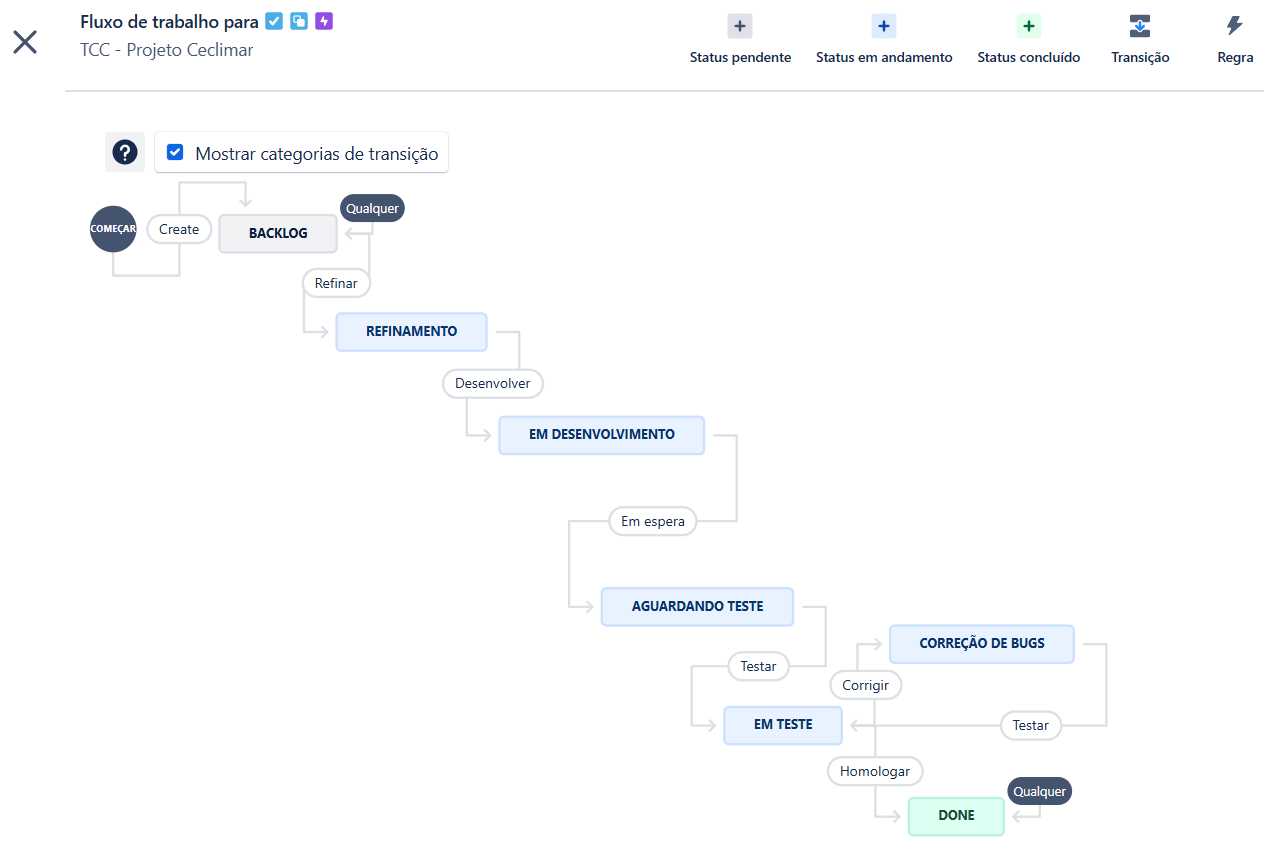
\includegraphics[width=0.8\textwidth]{imagens/fluxoJira.png}
    \caption{Fluxo de trabalho do Jira gerado para o desenvolvimento do projeto.}
    \legend{Fonte: Autor}
    \label{fig:fluxoJira}
\end{figure} 

O \textit{Backlog} é a coluna onde todas as tarefas, user stories e \textit{bugs} serão inicialmente posicionados. Nesta etapa, as tarefas serão priorizadas antes de andarem para o próximo estágio.

No Refinamento, as tarefas puxadas do \textit{Backlog} são detalhadas para um desenvolvimento mais assertivo. São refinados critérios de aceitação, estimativas de tempo e algum débito técnico.

As tarefas que estiverem em desenvolvimento são as que tiveram, efetivamente, o seu desenvolvimento iniciado. Assim que o desenvolvimento estiver finalizado, as tarefas serão transferidas para aguardando teste, onde ficarão até serem puxadas para testes mais detalhados.

No estágio de teste, os critérios de aceite e a presença de \textit{bugs} serão testados com o intuito de manter a qualidade do produto final. As tarefas que tiverem \textit{bugs} ou divergências de regras de negócio identificadas serão movidas para a coluna Correção de \textit{bugs} para que sejam corrigidas.

E, por último, após a homologação das tarefas nas etapas anteriores as tarefas são movidas para \textit{Done} que indicará sua finalização.

% ---

% ---
% Capitulo 3
% ---
\chapter{Estudo de Aplicações Correlatas}\label{trabalhos-correlatos}

Com o intuito de contextualizar e ter uma melhor visão de onde posicionar o projeto dentro do campo de pesquisa escolhido, foi realizada uma seleção de trabalhos correlatos, cujos principais critérios de aceitação incluíram a abordagem de temas como: monitoramento de fauna, desenvolvimento sustentável, gestão ambiental e ciência cidadã. Garantindo assim, relevância e alinhamento do projeto com as necessidades e avanços da área.

O ponto de partida para as pesquisas foi o \citeonline{sibbr2024}. A plataforma online, pertencente ao sistema gov.br \cite{govbr2024}, que integra dados e informações sobre a biodiversidade e os ecossistemas de diversas fontes, os tornando acessíveis e livres para usos diversos. Nele, também é possível ter acesso ao sistema Ciência Cidadã, que consiste em uma colaboração entre a comunidade e cientistas na coleta de dados para pesquisa científica. 

A partir do levantamento bibliográfico, pesquisas na plataforma Play Store \cite{playstore2024}, presente nos dispositivos Android \cite{android2024}, foram realizadas baseadas em alguns projetos e palavras-chave pré-selecionadas. As principais palavras-chave usadas para realizar as buscas foram: animais costeiros, coleta de dados, monitoramento ambiental, ciência cidadã.

Nesta seção, serão apresentadas três aplicações separadas no levantamento documental que  demonstraram possuir características e funcionalidades que podem auxiliar na definição e desenvolvimento deste sistema. Estas aplicações possuem algumas características em comum, porém cada uma delas também traz características únicas que serão importantes balizadoras nas tomadas de decisão deste projeto.

% ---
\section{SISS-Geo}\label{siss-geo}
% --- 

O Sistema de Informação em Saúde Silvestre (SISS-Geo) da FIOCRUZ é desenvolvido pela Plataforma Institucional Biodiversidade e Saúde Silvestre, com apoio do Laboratório Nacional de Computação Científica. É gratuito, disponível em \textit{smartphones} e na \textit{web}, para o monitoramento da saúde dos animais silvestres em ambientes naturais, rurais e urbanos. Apoia a investigação da ocorrência de agentes causadores de doenças, como agentes infecciosos, que podem acometer pessoas e animais. Como instrumento de ciência cidadã torna possível, a partir de registros realizados por cidadãos comuns, profissionais de saúde, meio ambiente, pesquisadores e especialistas em vida silvestre, agir para a prevenção e controle de zoonoses e a conservação da biodiversidade brasileira \cite{chame2015sissgeo}.

\begin{figure}[htb]
  \centering
  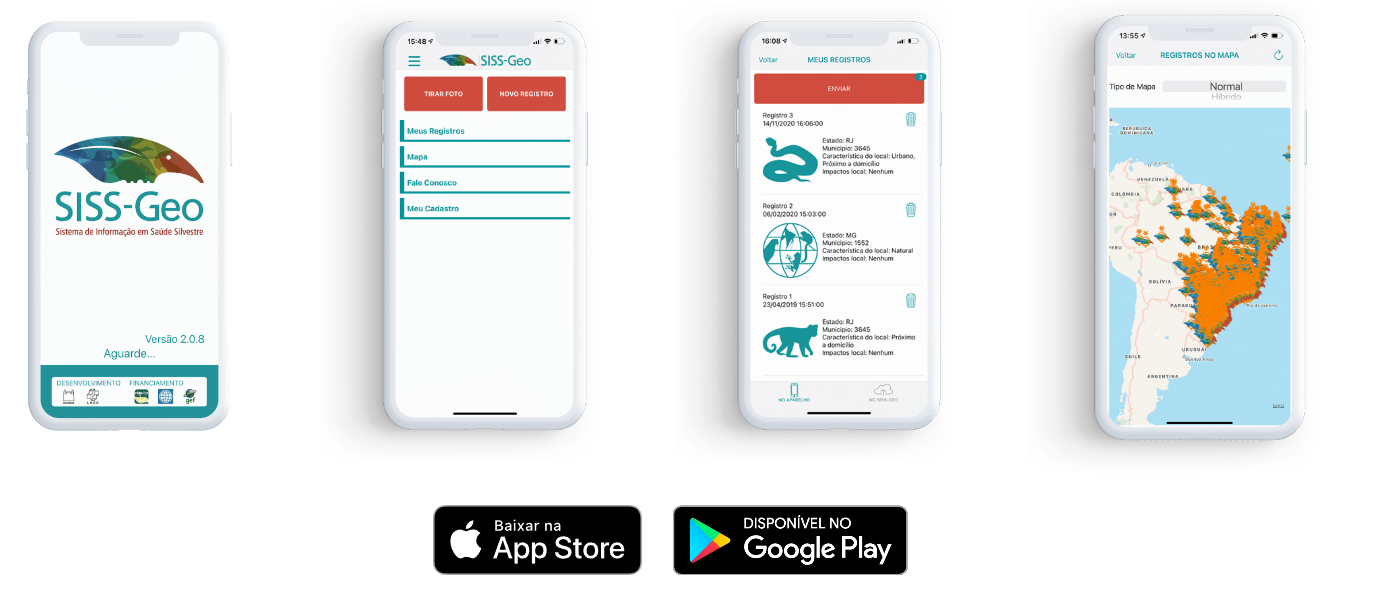
\includegraphics[width=1\textwidth]{imagens/sisGeoApp.png}
  \caption{Interface do sistema SISS-Geo.}
  \legend{Fonte: \citeonline{plataforma2024sissgeo}.}
  \label{fig:sisgeoApp}
\end{figure}

A aplicação \textit{mobile} foi lançada em 2014 e está disponível tanto para iOS quanto para Android (Figura~\ref{fig:sisgeoApp}) e possui mais de 10.000 downloads, com avaliação média de 4,7/5 baseada em 116 avaliações de usuários. Foram registrados, até 26 de março de 2024, 33 mil registros e quase 13 mil usuários colaboradores.

O sistema é bem consolidado e amplamente utilizado no Brasil, possuindo uma ótima aceitação entre especialistas e cidadãos em diversas regiões do país. Apesar de possuir opções para identificação de dados da fauna costeira, estes se mostram limitados quando comparados com os demais biomas. Ao alterar a escala de análise, é possível perceber, com um recorte mais detalhado do cordão litorâneo, que este não é o principal foco da aplicação e, atualmente, ela possui uma participação muito maior nas regiões continentais (Figura~\ref{fig:sisgeoMap}).

\begin{figure}[htb]
  \centering
  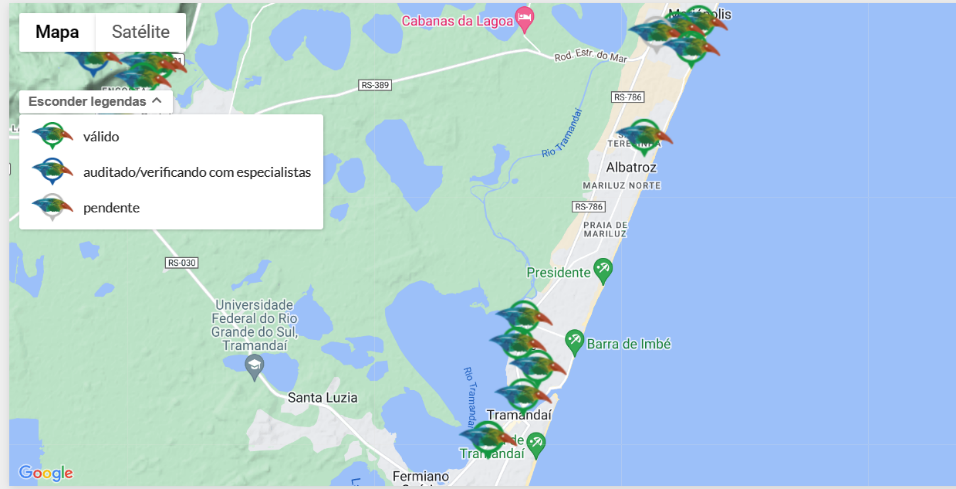
\includegraphics[width=1\textwidth]{imagens/sisGeoMapa.png}
  \caption{Recorte da região costeira do litoral norte do Rio Grande do Sul.}
  \legend{Fonte: \citeonline{plataforma2024sissgeo}.}
  \label{fig:sisgeoMap}
\end{figure}

Principais pontos fortes: funcionalidade \textit{offline}, iniciativa ambiental de grande contribuição, aplicação leve, ideia colaborativa de preservação, georreferenciamento de dados com boa visualização.

Entre as principais reclamações dos usuários estão: sistema pouco intuitivo, poucas opções de animais pré-cadastrados, interface confusa com formulário por vezes muito técnico.

% ---
\section{Sistema Urubu}\label{urubu}
% --- 

O Sistema Urubu é uma iniciativa do Centro Brasileiro de Ecologia de Estradas da UFLA, sob a coordenação do professor Alex Bager. Criado em 2014, o aplicativo de ciência cidadã é a maior rede para conservação da biodiversidade brasileira, destinada à coleta e gestão de informações de fauna selvagem ao longo de rodovias e ferrovias no Brasil. 

A aplicação permite que voluntários enviem registros de animais atropelados e infraestruturas viárias por meio de aplicativo móvel, enquanto especialistas validam e caracterizam esses registros para torná-los confiáveis. Os dados coletados são centralizados em um banco de dados e disponibilizados em um Sistema de Informações Geográficas, facilitando a visualização e análise pelos usuários. O Sistema Urubu também oferece ferramentas como o Urubu \textit{web}, para gestão e validação dos dados, e o Urubu Map, para visualização geográfica dos registros \cite{castro2019sistema}. Ao longo de seus anos de existência, o sistema reuniu mais de 25 mil usuários e 150 mil registros de animais atropelados em todo o território brasileiro, demonstrando seu impacto e relevância na conservação da biodiversidade.

\begin{figure}[htb]
  \centering
  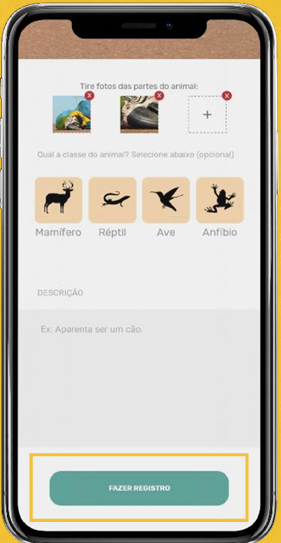
\includegraphics[width=0.33\textwidth]{imagens/app1.png}
  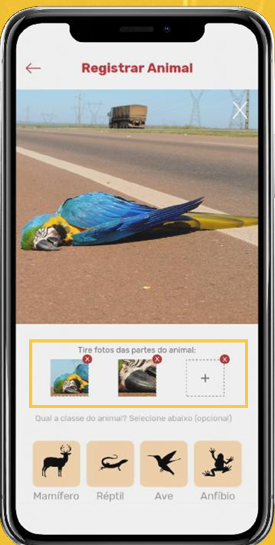
\includegraphics[width=0.323\textwidth]{imagens/app3.png}
  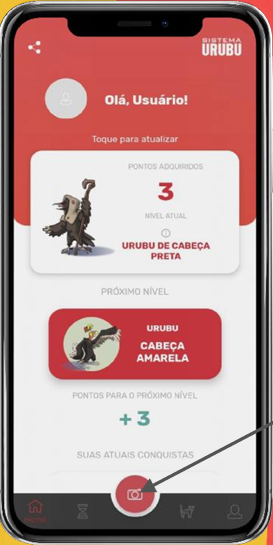
\includegraphics[width=0.32\textwidth]{imagens/app2.png}
  \caption{Interface do Sistema Urubu.}
  \legend{Fonte: Capturas de tela do sistema urubu disponíveis no manual de uso do aplicativo.}
  \label{fig:urubuApp}
\end{figure}

O Sistema Urubu apresenta uma interface amigável e um fluxo de obtenção e envio de dados de registros intuitivo (Figura~\ref{fig:urubuApp}.a e ~\ref{fig:urubuApp}.b), além de um fluxo gamificado com progressão recompensada para os usuários que contribuem com o projeto (Figura~\ref{fig:urubuApp}.c).

O fluxo de funcionamento da aplicação se inicia com a morte de algum animal em uma rodovia ou ferrovia, quando esse animal é encontrado por usuário a entrada de registro pode ser realizada via \textit{mobile}, \textit{web} ou por importação via planilha de Excel. Os dados de cada registro são então passados por uma análise de profissionais que decidirão se serão inseridos nos dados finais.

Apesar de ter alcançado importantes números de aceitação e uso entre 2014 e 2023, atualmente o sistema se encontra desativado e indisponível para download em todas as plataformas e seu site se encontra fora do ar.

Em contato com o coordenador do projeto Alex Bager por e-mail, foi informado de que o Sistema Urubu foi desativado devido a falta de recursos. Segundo seu relato, além dos custos para manter a aplicação no ar com investimentos contínuos, os aplicativos de ciência cidadã requerem muita comunicação e relacionamento com os participantes, o que torna a estrutura mais complexa e custosa.

% ---
\section{SIMBA}\label{simba}
% --- 

O Sistema de Monitoramento da Biota Aquática (SIMBA), é um sistema \textit{web} de gerenciamento de dados criado pelo Laboratório de Oceanografia Biológica da UNIVALI com a finalidade de armazenar dados coletados por instituições executoras dos projetos de monitoramentos de praias. O desenvolvimento do SIMBA se iniciou para auxiliar nos fluxos de dados entre os atores sociais envolvidos nos Projetos de Monitoramento de Praias (PMPs) e fazer com que os dados obtidos sejam disponibilizados e divulgados para a população.

Os PMPs são desenvolvidos para o atendimento de condicionantes de licenciamento ambiental federal, conduzido pelo IBAMA, de atividades de exploração e produção de petróleo e gás natural de bacias \textit{offshore} sob atuação da Petrobras. Estes projetos tem o objetivo de avaliar as possíveis interferências na área de abrangência dos projetos, analisando tanto tetrápodes marinhos (aves, tartarugas e mamíferos) por meio do monitoramento das praias, atendimento veterinário aos animais debilitados e da coleta de dados de animais mortos, quanto resíduos sólidos encontrados \cite{petrobras_simba_2024}.

Atualmente os projetos estão presentes nas bacias de Santos, Campos, Espírito Santo, Sergipe-Alagoas e Potiguar.

\begin{figure}[htb]
  \centering
  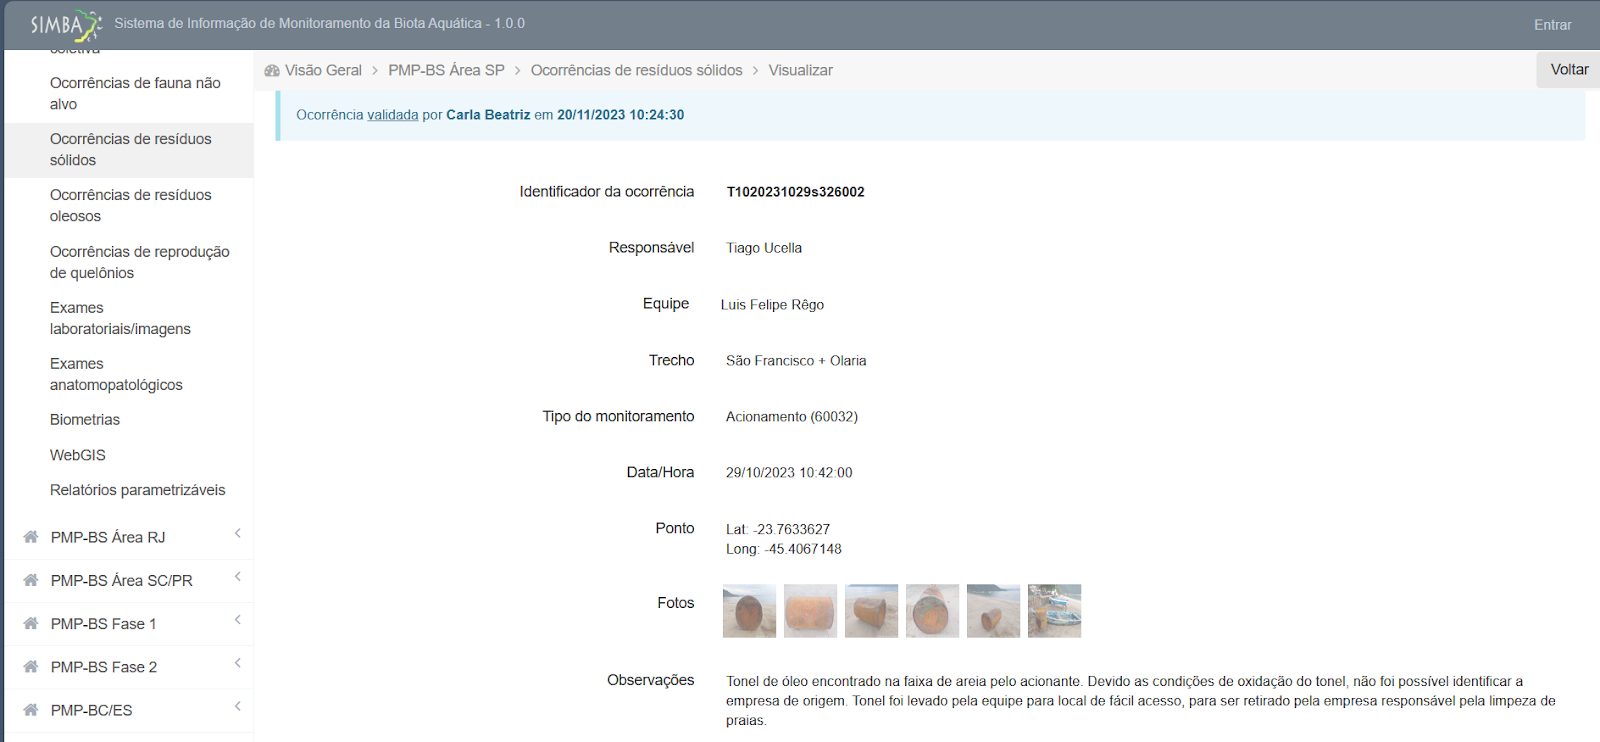
\includegraphics[width=1\textwidth]{imagens/simbaRegistro.png}
  \caption{Captura de tela de uma página \textit{web} de registro de visualização de ocorrências cadastradas no SIMBA.}
  \legend{Fonte: \cite{petrobras_simba_2024}.}
  \label{fig:simbaRegistro}
\end{figure}

O SIMBA conta com funcionalidades de cadastro de ocorrências de fauna, resíduos sólidos (Figura~\ref{fig:simbaRegistro}), exames, jornadas de campo com os caminhamentos realizados. Os pontos de ocorrência de cada cadastro são georreferenciados, assim como as jornadas de monitoramento, gerando mapas para melhor visualização e análise dos dados (Figura~\ref{fig:simbaMonitoramento}).

\begin{figure}[htb]
  \centering
  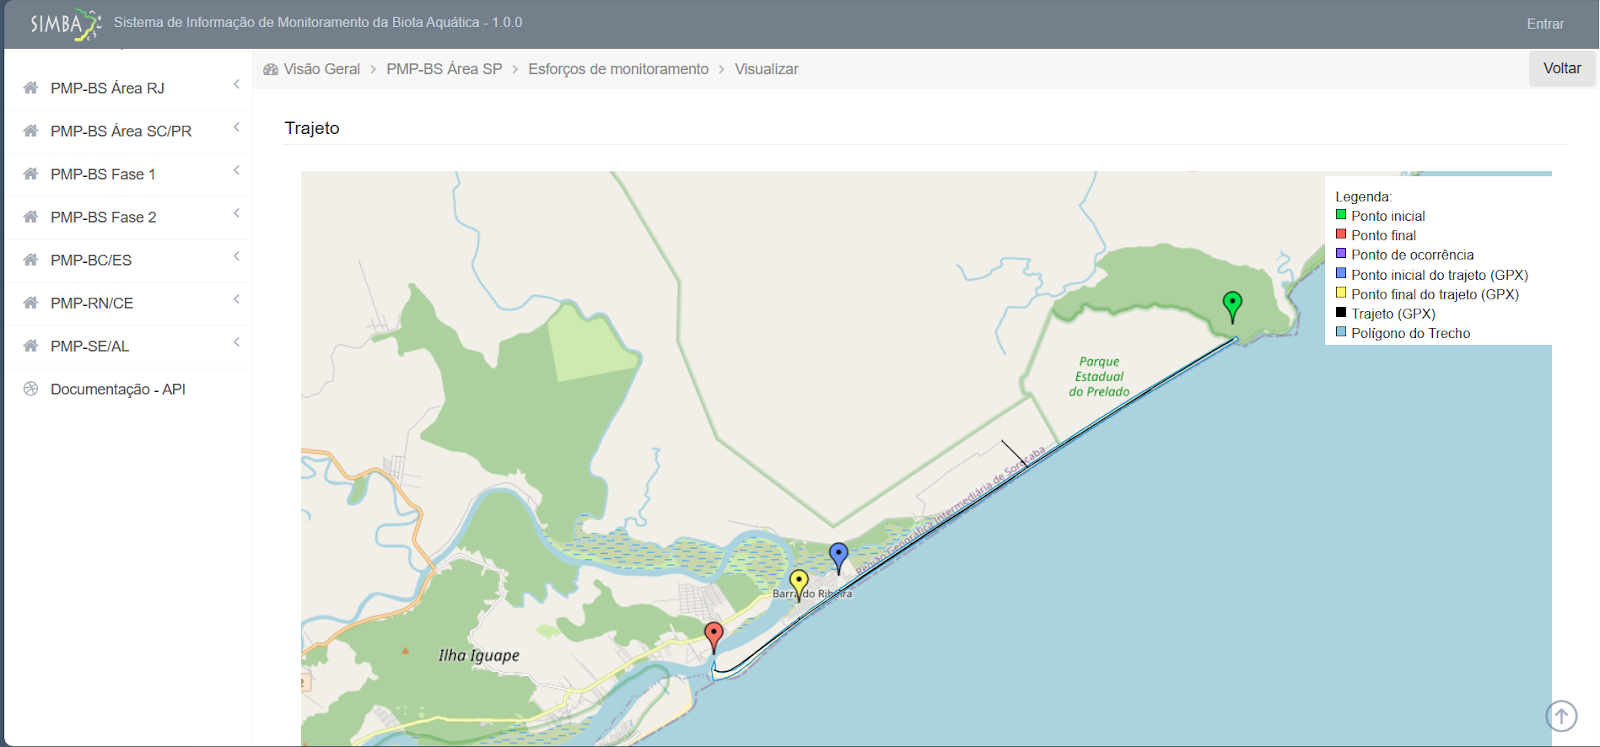
\includegraphics[width=1\textwidth]{imagens/simbaTrajetoria.png}
  \caption{Captura de tela de um mapa georreferenciado gerado a partir dos dados de jornada de monitoramento cadastrado no SIMBA.}
  \legend{Fonte: \cite{petrobras_simba_2024}.}
  \label{fig:simbaMonitoramento}
\end{figure}

O sistema possui uma área de acesso liberada ao público onde é possível visualizar dados já levantados e validados e uma área de acesso restrito liberada para pesquisadores. Possui uma interface mais limpa e direta, atendendo a um estilo de aplicação profissional apenas com o conteúdo necessário (Figura~\ref{fig:simbaPaginaCadastro}). Os dados são bem organizados e acessíveis para quem estiver interessado em acompanhar os estudos e evidências coletadas. Porém, para leigos essa interface pode, inicialmente, trazer um pouco de estranheza devido ao visual menos apelativo e aos termos mais científicos apresentados.

\begin{figure}[htb]
  \centering
  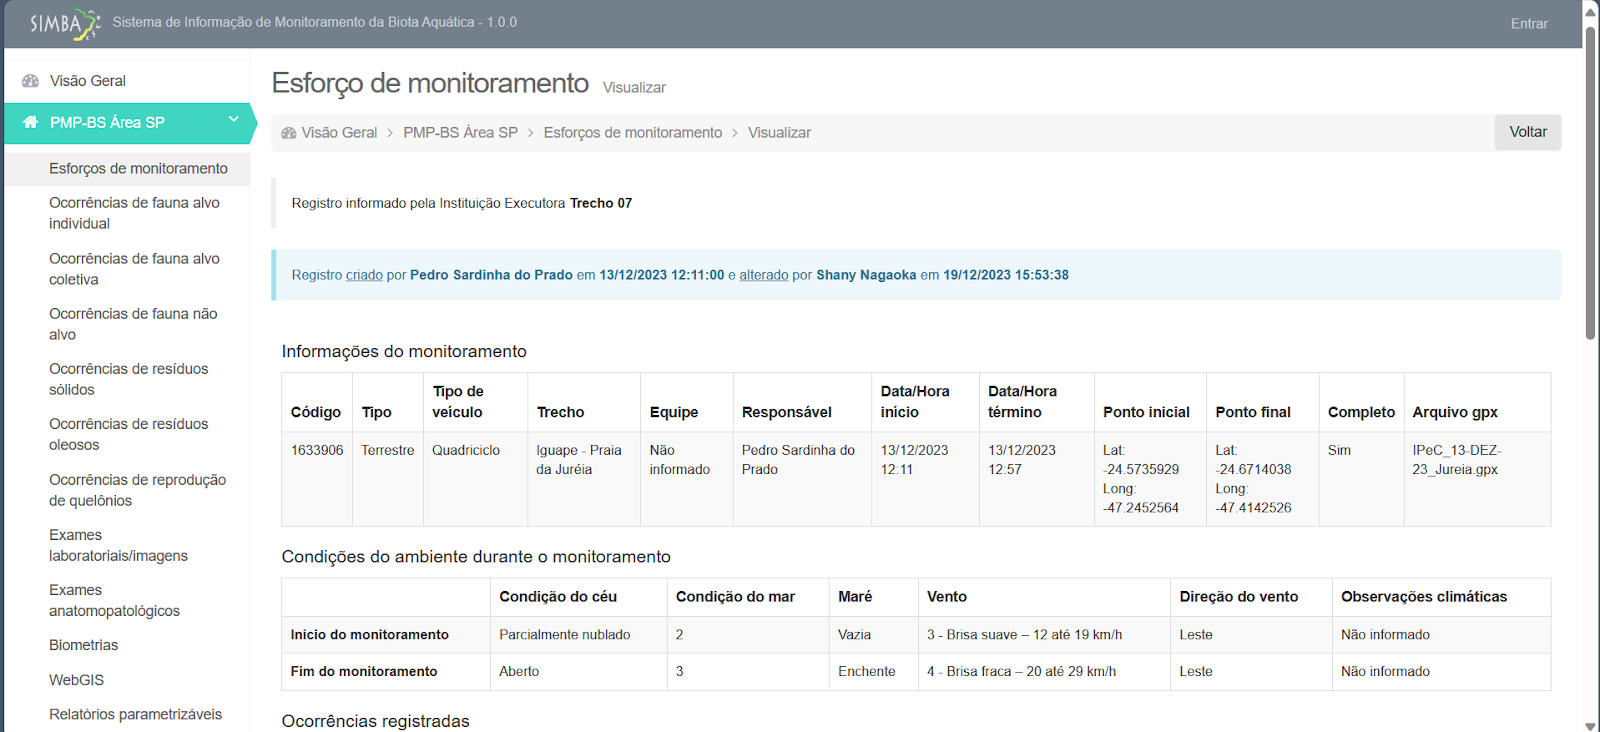
\includegraphics[width=1\textwidth]{imagens/simbaMonitoramento.png}
  \caption{Captura de tela da página \textit{web} de monitoramento cadastrada no SIMBA.}
  \legend{Fonte: \cite{petrobras_simba_2024}.}
  \label{fig:simbaPaginaCadastro}
\end{figure}

A geração de mapas georreferenciados e a possibilidade de uso \textit{offline} são aspectos importantes a serem destacados, pois permitem uma melhor análise e acompanhamento gráfico dos dados coletados e possibilitam que estes dados sejam obtidos até mesmo em locais mais isolados sem conexão com a internet. Outra função interessante é a liberação de dados para o público geral que se mostrar interessado em acompanhar os resultados e andamentos dos estudos nas praias onde os PMPs estão sendo realizados.

\section{Análise Comparativa e Direcionamentos do Projeto}

Com a análise dos principais trabalhos correlatos existentes, foi possível levantar os principais pontos de sucesso e alguns aspectos que precisam de melhorias, os quais influenciam diretamente na capacidade de sistemas similares alcançarem seus objetivos e obterem a aceitação do público-alvo.

A receptividade do Sistema Urubu e do SISS-Geo indicou um interesse significativo da população em participar de projetos de ciência cidadã, evidenciado pelos números expressivos de \textit{downloads} e registros de dados apresentados anteriormente.

Cada um dos três sistemas possui suas peculiaridades e objetivos distintos: enquanto o SISS-Geo está mais voltado ao monitoramento da saúde de animais silvestres e à investigação de agentes causadores de doenças, o Sistema Urubu foca principalmente no monitoramento de animais atropelados em rodovias e ferrovias. Por sua vez, o SIMBA busca fornecer visibilidade ao monitoramento costeiro realizado em regiões de exploração e produção de petróleo.

Sendo assim, a partir da análise prévia, foi possível constatar que existe uma oportunidade de posicionamento para o sistema proposto neste projeto, que se enquadra como uma plataforma com interface amigável e intuitiva, visando otimizar o processo de coleta, classificação e gestão de dados da fauna costeira. O sistema poderá se apoiar em pontos fortes identificados nos sistemas correlatos, como a funcionalidade offline do SISS-Geo, a interface amigável do Sistema Urubu e a organização dos dados do SIMBA.

O sistema proposto buscará oferecer uma experiência de usuário agradável e descomplicada para o registro de observações da fauna costeira, com opções abrangentes de espécies para classificação e ferramentas de visualização de dados claras e acessíveis. Ao adotar uma abordagem centrada no usuário e priorizar a simplicidade e eficiência, pretende-se ampliar o engajamento da comunidade na coleta de dados científicos e contribuir significativamente para o monitoramento e conservação da biodiversidade costeira.

% ---

% Capitulo 4
% ---

\chapter{Referencial Teórico}\label{referencial-teorico}

% ---
\section{Ciência Cidadã}
% ---

A Ciência Cidadã representa uma ponte entre a comunidade científica e o público geral, permitindo que pessoas sem formação científica formal possam contribuir em pesquisas científicas. Essa metodologia colaborativa tem se destacado em diversas áreas de pesquisa como na conservação da biodiversidade e na preservação ambiental. Através da Ciência Cidadã é possível que voluntários coletem e analisem dados, fornecendo informações que agregam no conhecimento acadêmico e auxiliam na resolução de questões sociais.

Segundo \citeonline{palma2016monitoramento}, trata-se de uma metodologia de pesquisa promissora na produção de conhecimento para ser aplicada em diversos campos científicos. Essa abordagem se destaca, em especial, com seu potencial de  geração de dados e análises, temporal e espacial, quando comparada com os métodos tradicionais de pesquisa. Para \citeonline{wildschut2017citizen}, a metodologia da ciência cidadã tem potencial para ampliar o escopo de pesquisas e aumentar e aprimorar a capacidade na coleta de dados e que os cidadãos que participam podem contribuir com informações importantes enquanto aprendem sobre as mais diversas áreas científicas.

A construção de conhecimento colaborativo realizado entre cidadãos e cientistas se mostra uma maneira poderosa de construção de conhecimentos, que agrega tanto no meio científico quanto social. Estes projetos instigam que as pessoas participem de maneira voluntária e ativa na resolução de situações do dia-a-dia da nossa sociedade, disseminando conhecimento de diversas áreas e fazendo com que diversos conteúdos saiam de suas bolhas científicas e obtenham um alcance maior.

% ---
\section{Agenda 2030}
% ---

A Agenda 2030 para o Desenvolvimento Sustentável é um plano de ação global adotado pelas Nações Unidas em 2015, com o objetivo de promover a prosperidade enquanto protege o planeta. Ela estabelece 17 Objetivos de Desenvolvimento Sustentável (ODS), que são subdivididos em 169 metas específicas. Esses objetivos englobam uma ampla gama de questões sociais, econômicas e ambientais, como erradicação da pobreza, igualdade de gênero, educação de qualidade, água limpa e saneamento, energia acessível e não poluente, trabalho decente e crescimento econômico \cite{onu2015ods}.

Segundo a organização, os ODS são projetados com os três pilares do desenvolvimento sustentável: econômico, social e ambiental. A Agenda enfatiza a importância de garantir que os direitos humanos de todos sejam realizados e que haja igualdade de gênero e empoderamento de mulheres e meninas. Além disso, reconhece que a erradicação da pobreza em todas as suas formas é o maior desafio global e, um requisito indispensável para o desenvolvimento sustentável.

A implementação da Agenda 2030 requer a mobilização de recursos e uma Parceria Global para o Desenvolvimento Sustentável, envolvendo todos os países, partes interessadas e pessoas. A Agenda é mundial, e se aplica a todos os países levando em conta diferentes realidades nacionais, capacidades e níveis de desenvolvimento. Ela promove a paz, justiça e instituições eficazes, e destaca a necessidade de ações urgentes sobre a mudança climática para proteger o planeta para as gerações presentes e futuras \cite{onu2015agenda2030}.

% ---
\section{Objetivos de Desenvolvimento Sustentável (ODS)}
% ---

Os ODS são um conjunto de 17 metas estabelecidas pelas Nações Unidas para abordar os principais desafios de desenvolvimento no Brasil e em todo o mundo. Esses objetivos visam criar um futuro mais justo, equitativo e sustentável para todos \cite{onu2015ods}. São eles:

\begin{itemize}
    \item \textbf{ODS 1}: Erradicação da Pobreza: Acabar com a pobreza em todas as suas formas, em todos os lugares.
    \item \textbf{ODS 2}: Fome Zero e Agricultura Sustentável: Garantir a segurança alimentar, melhorar a nutrição e promover a agricultura sustentável.
    \item \textbf{ODS 3}: Saúde e Bem-Estar: Assegurar uma vida saudável e promover o bem-estar para todas as idades.
    \item \textbf{ODS 4}: Educação de Qualidade: Garantir uma educação inclusiva, equitativa e de qualidade.
    \item \textbf{ODS 5}: Igualdade de Gênero: Alcançar a igualdade de gênero e empoderar todas as mulheres e meninas.
    \item \textbf{ODS 6}: Água Limpa e Saneamento: Garantir a disponibilidade e gestão sustentável da água e saneamento para todos.
    \item \textbf{ODS 7}: Energia Limpa e Acessível: Assegurar o acesso a fontes de energia acessíveis, confiáveis, sustentáveis e modernas.
    \item \textbf{ODS 8}: Trabalho Decente e Crescimento Econômico: Promover o crescimento econômico inclusivo e sustentável, emprego pleno e produtivo e trabalho decente para todos.
    \item \textbf{ODS 9}: Indústria, Inovação e Infraestrutura: Construir infraestruturas resilientes, promover a industrialização inclusiva e sustentável e fomentar a inovação.
    \item \textbf{ODS 10}: Redução das Desigualdades: Reduzir as desigualdades dentro e entre países.
    \item \textbf{ODS 11}: Cidades e Comunidades Sustentáveis: Tornar as cidades e os assentamentos humanos inclusivos, seguros, resilientes e sustentáveis.
    \item \textbf{ODS 12}: Consumo e Produção Responsáveis: Assegurar padrões de consumo e produção sustentáveis.
    \item \textbf{ODS 13}: Ação Contra a Mudança Global do Clima: Tomar medidas urgentes para combater a mudança climática e seus impactos.
    \item \textbf{ODS 14}: Vida na Água: Conservar e usar de forma sustentável os oceanos, mares e recursos marinhos.
    \item \textbf{ODS 15}: Vida Terrestre: Proteger, restaurar e promover o uso sustentável dos ecossistemas terrestres, gerir florestas de forma sustentável, combater a desertificação e deter a perda de biodiversidade.
    \item \textbf{ODS 16}: Paz, Justiça e Instituições Eficazes: Promover sociedades pacíficas e inclusivas para o desenvolvimento sustentável, proporcionar acesso à justiça para todos e construir instituições eficazes, responsáveis e inclusivas em todos os níveis.
    \item \textbf{ODS 17}: Parcerias e Meios de Implementação: Fortalecer os meios de implementação e revitalizar a parceria global para o desenvolvimento sustentável.
\end{itemize}

Os itens acima são um apelo global visando acabar com a pobreza, proteger o meio ambiente e o clima e garantir que as pessoas, em todos os lugares, possam desfrutar de paz e de prosperidade. São objetivos nos quais as Nações Unidas estão contribuindo para atingir a Agenda 2030 no Brasil \cite{onu2015ods}.

% ---
\section{Metodologia Iterativa Incremental}
% ---
A metodologia iterativa incremental é uma abordagem de desenvolvimento de \textit{software} que divide o processo em ciclos repetitivos. Cada iteração resulta em uma versão incrementada do \textit{software}, que é construída sobre a versão anterior com adições e melhorias. Segundo \citeonline{pressman2011engenharia}, essa metodologia permite que as equipes avaliem e integrem feedbacks mais rapidamente, adaptando-se às mudanças e refinando o produto ao longo do tempo. Isso contrasta com o modelo tradicional em cascata, onde cada fase deve ser concluída antes da próxima começar, sem retorno para fases anteriores.

De acordo com \citeonline{pressman2011engenharia}, o modelo incremental é uma abordagem de desenvolvimento de \textit{software} que foca na entrega gradual de funcionalidades em sucessivas versões incrementais. Nesse modelo, o desenvolvimento do \textit{software} é dividido em várias partes ou incrementos, cada um entregando uma versão operante do produto, que é aprimorada e expandida em lançamentos subsequentes.

\citeonline{pressman2011engenharia} afirma que o modelo incremental integra elementos de fluxos de processos lineares e paralelos. Na Figura~\ref{fig:incremental} é possível observar essa relação a partir das sequências lineares de forma escalonada que demonstram que ao longo do tempo cada incremento adiciona funcionalidades ou aprimoramentos ao sistema, permitindo uma evolução constante e contínua do produto final.

\begin{figure}[htb]
  \centering
  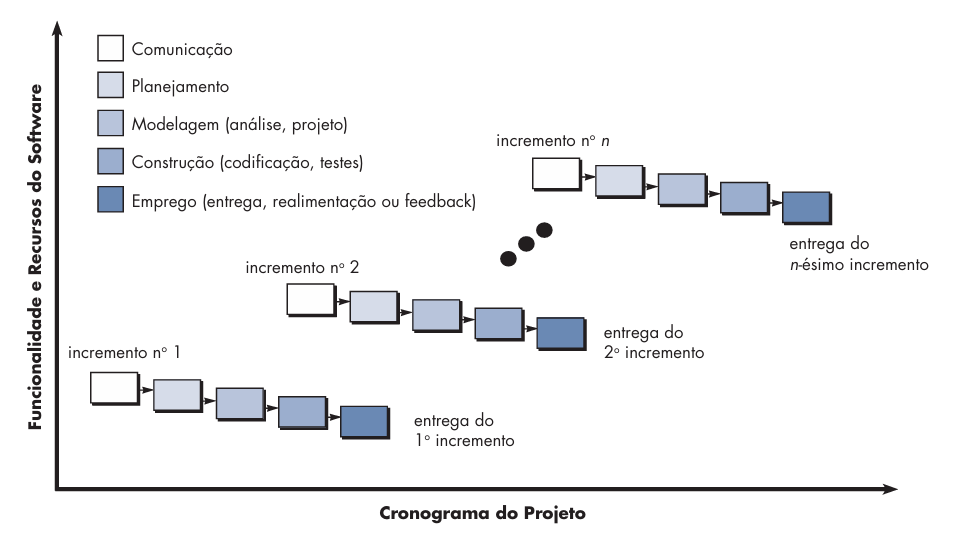
\includegraphics[width=0.8\textwidth]{imagens/graficoPressman.png}
  \caption{Ciclo de desenvolvimento incremental.}
  \legend{Fonte: \citeonline{pressman2011engenharia}.}
  \label{fig:incremental}
\end{figure}

% ---
\section{Kanban}
% ---

O Kanban é um método de gestão de fluxo de trabalho que fornece uma visualização das tarefas que devem ser realizadas, quando entregá-las e quanto ainda é necessário para finalizá-las com o objetivo de aumentar a eficiência e o entendimento do desenvolvimento \cite{ohno1988toyota}. Originou-se no sistema da Toyota no Japão dos anos 1940 e foi adaptado para o desenvolvimento de \textit{software} e sistemas de TI por David J. Anderson em 2004. Para isso, o Kanban utiliza de um quadro dividido em colunas para representar os diferentes estágios do trabalho, onde os cartões que representam as tarefas se movem de uma coluna para outra, refletindo o progresso real \cite{zayat2020framework}.

% ---
\section{Jira}
% ---

O \textit{Jira} é um \textit{software} comercial de gerenciamento de projetos desenvolvido pela empresa Atlassian. Ele permite a criação, acompanhamento e gerência de tarefas e projetos a partir de uma interface personalizável que suporta diversas metodologias ágeis como Scrum e Kanban, facilitando a colaboração e comunicação durante o desenvolvimento.

A ferramenta pode ser usada para planejar \textit{sprints}, atribuir tarefas, acompanhar \textit{bugs}, gerar relatórios e analisar o desempenho da equipe. Ele possui integração com uma variedade de ferramentas de desenvolvimento e oferece funcionalidades para personalizar fluxos de trabalho, campos e painéis, tornando-o adaptável às necessidades específicas de cada projeto ou organização.


\section{Tecnologias e Frameworks}\label{tecnologias}

Neste capítulo, serão apresentadas as tecnologias escolhidas para o 
desenvolvimento do aplicativo, destacando os aspectos que influenciaram nas 
escolhas e como elas contribuíram para o desenvolvimento do projeto.

\subsection{Flutter}

O \textit{Flutter} é um conjunto de ferramentas de UI (Interface do Usuário) criado 
pelo \textit{Google} em 2017. Se diferencia por possuir um suporte multiplataforma de código aberto 
projetado para permitir a reutilização de código em diversos sistemas operacionais, como \textit{iOS}, 
\textit{Android}, \textit{web} e \textit{desktop}, enquanto possibilita que as aplicações interajam 
diretamente com os serviços de cada plataforma. Como publicado por seus desenvolvedores, 
o \textit{Flutter} oferece 
uma solução centralizada para o desenvolvimento multiplataforma que facilita a criação de 
componentes visuais ao mesmo tempo em que realiza a integração com recursos nativos de cada tipo 
de dispositivo \cite{flutterDocs2025}.

Com esse \textit{framework}, os aplicativos são compilados a partir de um único código-base para as 
plataformas \textit{mobile}, \textit{web} e \textit{desktop}. O desenvolvimento no \textit{Flutter} é baseado em \textit{Widgets}, 
componentes escritos em \textit{Dart} que são responsáveis pela visualização das telas e pela interação 
com o usuário.
Esses componentes podem ou não estar associados a um estado, quando estão, são chamados de \textit{Stateful} 
\textit{Widgets} e, quando não, de \textit{Stateless} \textit{Widgets} \cite{flutterDocs2025}.

Além disso, o \textit{Flutter} possui a funcionalidade de \textit{hot reload}. 
Uma ferramenta que permite que alterações sejam feitas no código 
enquanto a aplicação está em execução, gerando uma 
atualização em tempo real da interface do usuário e da lógica da aplicação, 
mantendo inalterado seu estado de execução.

A escolha pelo \textit{Flutter} (versão 3.29.2) se deu principalmente pela sua capacidade multiplataforma a partir de 
uma única base de código, otimizando tempo e recursos. Outro fator decisivo foi a 
facilidade de integração com os diversos serviços do \textit{Firebase}, 
que facilitam a implementação de funcionalidades essenciais,  
como a autenticação, o banco de dados em tempo real e o armazenamento.

\subsection{Dart}

\textit{Dart} é uma linguagem de programação lançada pelo \textit{Google} em 2013, criada com foco em produtividade e 
performance para aplicações multiplataforma. A linguagem é orientada a objetos e oferece tipagem 
estática forte, porém também é possível optar pelo uso de tipagem dinâmica, 
o que pode ser útil em algumas situações. \cite{dartDocs2025}.

Um aspecto importante do \textit{Dart} é sua flexibilidade de compilação. 
É uma linguagem que utiliza tanto a compilação \textit{just-in-time} 
(JIT) quanto \textit{ahead-of-time} (AOT). 
Em tempo de desenvolvimento, o \textit{Dart} roda no \textit{Dart} VM 
usando JIT, o que permite recompilar apenas partes 
do código em tempo real sem reiniciar toda a aplicação. Essa funcionalidade 
viabiliza o recurso de \textit{hot reload} do \textit{Flutter}, permitindo 
que alterações sejam refletidas imediatamente na aplicação sem alterar o 
estado da interface.
Após realizar o lançamento de uma versão, o \textit{Dart} usa AOT para compilar o código diretamente 
para código nativo, o que garante um desempenho maior com relação ao JIT \cite{dartDocs2025}.

A escolha do Dart (versão 3.7.2) como linguagem de programação para o projeto se deu pela sua
proximidade com o \textit{Flutter}, pela tipagem forte, pelas características de 
programação orientada a objetos e pela facilidade de integração com o \textit{Firebase}.

\subsection{Firebase}

O \textit{Firebase} é uma plataforma de desenvolvimento de aplicativos móveis e \textit{web} 
fornecida pelo \textit{Google}, que oferece uma ampla gama de serviços \textit{backend} para 
facilitar a criação de aplicações robustas e escaláveis. Tem como característica 
permitir o desenvolvimento centralizado sem a necessidade de infraestrutura própria, 
fornecendo soluções completas para autenticação de usuários, banco de dados em tempo real
, armazenamento de arquivos, envio de notificações, análises de uso e monitoramento de 
desempenho. Além disso, a plataforma integra ferramentas para teste, distribuição 
e acompanhamento do ciclo de vida do aplicativo com suporte multiplataforma \cite{firebase2025}.

Dentre os principais serviços disponibilizados no plano \textit{Spark} que foram 
utilizados no projeto, estão o \textit{Firebase Authentication}, 
que possibilita a autenticação de usuários via e-mail/senha e \textit{Google}, com suporte 
para até 50 mil usuários ativos mensais sem custo. O \textit{Firebase Analytics} que fornece 
relatórios detalhados sobre o comportamento e uso do aplicativo, permitindo a 
análise de métricas essenciais. O \textit{App Distribution} que possibilita a distribuição de versões 
de teste do aplicativo para usuários selecionados durante as fases de desenvolvimento e teste. 
Além do \textit{Cloud Firestore Database} que oferece até 1 GB de armazenamento, com limites diários de 50 
mil leituras, 20 mil gravações e 20 mil exclusões de documentos. E do \textit{Cloud Storage} que
disponibiliza 5 GB de armazenamento, 1 GB de download diário, além de 20 mil operações 
de upload e 50 mil operações de download por dia \cite{firebase2025}.

Neste projeto, o \textit{Firebase} foi escolhido para gerenciar a autenticação e o armazenamento de 
dados, utilizando o \textit{Firebase Authentication} para autenticar usuários com diferentes métodos de login e 
o \textit{Firebase Storage} para armazenar imagens, além do banco de dados NoSQL 
\textit{Cloud Firestore Database} para salvar os dados gerais do sistema e do Analytics para 
geração de \textit{dashboards} visando analisar o funcionamento geral da aplicação.
A definição pelo \textit{Firebase} se deu pela robustez e facilidade de integração com \textit{Flutter} 
oferecendo uma plataforma de backend eficiente e escalável. A aplicação foi construída com a 
utilização dos benefícios do plano \textit{Spark} descritos acima,
que, apesar de ser um plano gratuito, traz diversas ferramentas com limites de uso suficientemente 
altos para projetos iniciais.

\subsection{Pacotes e Plugins do Flutter}

Como o \textit{Flutter} possui uma arquitetura baseada em pacotes e \textit{plugins}, para o desenvolvimento 
de algumas funcionalidades específicas da aplicação proposta neste trabalho foram selecionados 
algumas dependências externas para facilitar e aumentar as possibilidades de desenvolvimento.

As dependências do projeto podem ser classificadas em três categorias. Bibliotecas puramente em Dart, 
que não interagem com \textit{APIs} nativas da 
plataforma, como \texttt{excel} (para manipulação de planilhas), \texttt{intl} (internacionalização 
e formatação de dados) e \texttt{diacritic} (remoção de acentos e caracteres especiais).

Plugins, que integram o código \textit{Dart} com \textit{APIs} nativas dos 
sistemas operacionais \textit{Android} e \textit{iOS}. Exemplos incluem \texttt{geolocator}
 (geolocalização), 
\texttt{image\_picker} (acesso à câmera e galeria) e \texttt{permission\_handler} (gerenciamento 
de permissões).

E as ferramentas auxiliares, que contribuem com a geração 
de código e automação de processos durante o desenvolvimento, como \texttt{hive\_generator} 
(geração de adaptadores para o \textit{Hive}) e \texttt{build\_runner} (execução de processos automáticos de 
geração de código).

Essas dependencias permitem incorporar funcionalidades reutilizáveis no projeto 
como renderização de mapas, autenticação com Firebase e diversos formatos de gráficos 
sem a necessidade de implementações manuais que seriam custosas e extensas. 
Além disso, possibilitam o acesso a recursos nativos dos dispositivo, como a 
geolocalização, gerenciamento de permissões, câmera e o armazenamento local no dispositivo.

A Tabela~\ref{tab:dependencias_flutter} apresenta todas as dependências utilizadas 
no projeto, especificando a versão de cada uma, bem como uma breve 
descrição de sua finalidade. Essa relação visa demonstrar a amplitude de recursos externos 
incorporados ao aplicativo e documentar as versões exatas para fins de controle de compatibilidade.

\begin{table}[H]
    \centering
    \caption{Dependências do Projeto \textit{Flutter}}
    \begin{tabular}{|p{4cm}|p{2.5cm}|p{8cm}|}
    \hline
    \textbf{Dependência} & \textbf{Versão} & \textbf{Descrição breve} \\ \hline
    flutter & sdk: flutter & Framework principal para desenvolvimento de apps móveis. \\ \hline
    flutter\_localizations & sdk: flutter & Suporte a localização (i18n) para Flutter. \\ \hline
    cupertino\_icons & \^{}1.0.2 & Ícones estilo iOS para Flutter. \\ \hline
    firebase\_core & \^{}3.8.1 & Inicialização e integração do Firebase. \\ \hline
    firebase\_auth & \^{}5.3.4 & Autenticação com Firebase. \\ \hline
    cloud\_firestore & \^{}5.4.4 & Integração com o banco Firestore. \\ \hline
    firebase\_analytics & \^{}11.3.3 & Monitoramento e análise de uso (analytics). \\ \hline
    firebase\_app\_check & \^{}0.3.2+5 & Segurança para apps usando Firebase. \\ \hline
    google\_sign\_in & \^{}6.2.2 & Autenticação via Google. \\ \hline
    persistent\_bottom\_nav\_bar & \^{}6.2.1 & Barra de navegação inferior persistente. \\ \hline
    image\_picker & \^{}1.1.2 & Seleção de imagens da galeria ou câmera. \\ \hline
    firebase\_storage & \^{}12.3.4 & Armazenamento de arquivos no Firebase. \\ \hline
    diacritic & \^{}0.1.3 & Remoção de acentos (diacríticos) de strings. \\ \hline
    provider & \^{}6.1.2 & Gerenciamento de estado simplificado. \\ \hline
    photo\_view & \^{}0.15.0 & Visualização de imagens com zoom e rotação. \\ \hline
    geolocator & \^{}13.0.2 & Geolocalização e rastreamento de posição. \\ \hline
    geocoding & \^{}3.0.0 & Geocodificação e reversa. \\ \hline
    phosphor\_flutter & \^{}2.1.0 & Ícones customizados da biblioteca Phosphor. \\ \hline
    url\_launcher & \^{}6.3.1 & Abertura de URLs externas (navegadores, apps, etc.). \\ \hline
    accordion & \^{}2.6.0 & Componente de interface tipo acordeão. \\ \hline
    cached\_network\_image & \^{}3.4.1 & Cache para imagens carregadas da web. \\ \hline
    hive & \^{}2.2.3 & Banco de dados local rápido e leve. \\ \hline
    hive\_generator & \^{}2.0.1 & Gerador de código para Hive. \\ \hline
    path\_provider & \^{}2.1.1 & Acesso a diretórios do sistema de arquivos. \\ \hline
    connectivity\_plus & \^{}5.0.2 & Detecção de status de conectividade (online/offline). \\ \hline
    build\_runner & \^{}2.4.8 & Utilitário para geração de código automático. \\ \hline
    skeletonizer & \^{}1.4.2 & Animação skeleton loader (placeholders enquanto carrega). \\ \hline
    badges & \^{}3.1.2 & Criação de badges/insígnias visuais. \\ \hline
    pie\_chart & \^{}5.4.0 & Gráficos de pizza. \\ \hline
    graphic & \^{}2.5.0 & Biblioteca de gráficos avançados. \\ \hline
    share\_plus & \^{}10.1.4 & Compartilhamento nativo de conteúdo. \\ \hline
    exif & \^{}3.0.1 & Leitura de dados EXIF de imagens. \\ \hline
    latlong2 & \^{}0.9.0 & Tipos de dados para latitude e longitude. \\ \hline
    open\_filex & \^{}4.3.4 & Abertura de arquivos em apps externos. \\ \hline
    excel & \^{}4.0.6 & Manipulação de arquivos Excel (.xlsx). \\ \hline
    flutter\_map & \^{}8.1.1 & Renderização de mapas (como o OpenStreetMap). \\ \hline
    intl & \^{}0.19.0 & Internacionalização e formatação de datas/números. \\ \hline
    permission\_handler & \^{}12.0.0+1 & Gerenciamento de permissões do sistema operacional. \\ \hline
    device\_info\_plus & \^{}11.3.3 & Informações detalhadas sobre o dispositivo. \\ \hline
    \end{tabular}
    \label{tab:dependencias_flutter}
    \legend{Fonte: Autor}
\end{table}
    
\subsubsection{Hive}

O Hive é um banco de dados leve e extremamente rápido, escrito inteiramente 
em \textit{Dart}, projetado para ser usado em aplicações Flutter e 
\textit{Dart} nativas. Ele segue o modelo de banco de dados chave-valor, 
oferecendo uma alternativa eficiente ao SQLite e a outros bancos de dados 
mais complexos, especialmente em contextos mobile \cite{hive2025}.

No projeto o Hive foi escolhido como opção de banco de dados local para armazenamento dos registros em momentos em que o dispositivo está offline, 
permitindo que até 40 registros sejam armazenados localmente e sincronizados assim que a conexão com a internet retornar.
A principal vantagem do Hive é a simplicidade e velocidade em dispositivos móveis.

\subsubsection{Flutter Map}
O \textit{Flutter Map} é um plugin gratuito, multiplataforma e de código aberto
que permite a renderização de mapas 
dentro de aplicativos \textit{Flutter}. Oferece uma interface fácil de usar 
para adicionar camadas, marcadores personalizados e interações em mapas.
Possui suporte de diversos provedores de mapas, como
\textit{OpenStreetMap}, \textit{Mapbox} e \textit{Google Maps}, 
permitindo que os desenvolvedores 
 escolham a fonte de dados que melhor atende às suas necessidades. 
 Além disso, ele oferece suporte a recursos avançados, como 
 geolocalização, desenho de rotas e manipulação de gestos do 
 usuário, adição de \textit{layers} \cite{flutter_map_doc}.
 
 Neste projeto, o \textit{Flutter Map} foi utilizado para renderizar o mapa
 com marcadores personalizados das localizações dos registros realizados 
 pelos usuários, permitindo uma visão geográfica dos dados coletados.

\subsubsection{Excel}

O \textit{excel} é uma biblioteca de código aberto para o
\textit{Dart} que permite a leitura e escrita de arquivos do Microsoft Excel 
no formato \textit{XLSX} com customizações avançadas de template \cite{excel_flutter}.
Neste projeto foi utilizada para construir a planilha de registros personalizada para download e compartilhamento.

\subsubsection{Graphic}

\textit{Graphic} é uma biblioteca de visualização de dados para \textit{Flutter}, 
baseada 
na Gramática de Gráficos de Leland Wilkinson. Com ela é possível criar gráficos 
personalizados de diversos tipos. Além disso, oferece suporte 
a interações avançadas como: seleção, legenda, tooltips, zoom, e animações 
para transições e carregamento dos gráficos \cite{graphic_flutter}.

A aplicação desta biblioteca no projeto foi pensada para gerar uma 
visualização gráfica dos dados de registos coletados para maior síntese de
algumas informações chaves.
Para o resultado final, foram gerados gráficos nos formatos de pizza e barras.

% ---

% Capitulo 6
% ---
\chapter{Resultados Obtidos}
Este capítulo demonstra os artefatos produzidos para o \textit{software}, incluindo 
as informações associadas desde a análise até os testes.

\section{Levantamento de Requisitos}

O levantamento de requisitos foi essencial para compreender as necessidades do projeto e orientar o 
desenvolvimento das funcionalidades do aplicativo. Segundo 
\citeonline{sommerville2011}, os requisitos de um sistema são as descrições do que o sistema deve 
fazer, os serviços que ele irá oferecer e suas restrições de funcionamento. Neste projeto, a 
definição dos requisitos prioritários para o MVP\footnote{MVP é a sigla para 
\textit{Minimum Viable Product} (Produto Mínimo Viável), um conceito que se refere à 
versão mais simples de um produto 
que ainda entrega valor ao usuário e permite validações com o mínimo de esforço e 
custo.} e das suas limitações foi orientada por reuniões 
com o coordenador do projeto Fauna Marinha RS, especialmente com base na experiência prática dos 
profissionais do CECLIMAR, que indicaram as funcionalidades mais relevantes para o sistema.

\subsection{Requisitos Funcionais}

Nesta seção, serão expostos os requisitos funcionais do sistema, que segundo 
\citeonline{guedesuml2} correspondem ao que o cliente quer que o sistema realize,
ou seja, as funcionalidades do software. Esses requisitos estão organizados em tabelas
distintas, apresentadas a seguir. A Tabela~\ref{tab:req-funcionais} sintetiza os 63 requisitos funcionais
da versão 2.3.6 do aplicativo, que é a versão mais atualizada até o momento da entrega deste relatório.
Durante o desenvolvimento, os requisitos foram revisados e atualizados conforme necessário,
com base em feedbacks e testes realizados.

\begin{longtable}{@{}p{1.5cm}p{13cm}@{}}
    \caption{Requisitos funcionais do sistema}\label{tab:req-funcionais}\\
        \toprule
        \textbf{Código} & \textbf{Descrição} \\ \hline
        \midrule
        \endfirsthead
        
        \toprule
        \textbf{Código} & \textbf{Descrição} \\ \hline
        \midrule
        \endhead
        
        \midrule
        \multicolumn{2}{r@{}}{(Continua na próxima página)} \\
        \endfoot
        
        \bottomrule
        \endlastfoot
    % usuario
    % registro
    RF01 & O sistema deve permitir o registro de novos usuários com e-mail e senha. \\ \hline
    RF02 & O sistema deve permitir o registro de novos usuários com conta Google integrada ao Firebase Authentication. \\ \hline
    RF03 & O sistema deve diferenciar dois tipos de usuários: cientista cidadão (user) e pesquisador (admin). \\ \hline
    RF04 & O sistema deve permitir que um pesquisador cadastre outro pesquisador, com geração automática de senha segura (8 dígitos alfanuméricos e caracteres especiais). \\ \hline
    RF05 & O sistema deve permitir que um pesquisador conceda a outro usuário que já possui conta a role de pesquisador. \\ \hline

    % login
    RF06 & O sistema deve permitir o login via Firebase Authentication com e-mail e senha. \\ \hline
    RF07 & O sistema deve permitir o login via conta Google integrada ao Firebase Authentication. \\ \hline
    RF08 & O sistema deve unificar dados quando uma conta possui ambos os métodos de login. \\ \hline
    RF09 & O sistema deve permitir redefinição de senha através do fluxo do Firebase Authentication (envio de e-mail de redefinição). \\ \hline
    RF10 & O sistema deve permitir a recuperação da senha. \\ \hline
    RF11 & O sistema deve permitir que o usuário faça logoff. \\ \hline

    % exclusao de conta
    RF12 & O sistema deve permitir a exclusão da conta do usuário, independente do método de cadastro. \\ \hline
    RF13 & O sistema deve manter os registros realizados pelo usuário mesmo após a exclusão da conta, 
    para preservação de dados científicos. \\ \hline

    % editar perfil
    RF14 & O sistema deve permitir atualização do perfil de usuário cadastrado com e-mail e senha (nome, foto, e-mail). \\ \hline
    
    % tela de meu perfil
    RF15 & O sistema deve permitir ao usuário visualizar e gerenciar seu perfil. \\ \hline
    RF16 & O sistema deve possuir um conjunto de conquistas para cada usuário. \\ \hline
    RF17 & O sistema deve permitir ao usuário visualizar os últimos registros do seu perfil. \\ \hline
    RF18 & O sistema deve permitir ao usuário visualizar a quantidade total de registros realizadas por ele. \\ \hline

    % envio de registros
    RF19 & O sistema deve permitir envio de registros "simples". \\ \hline
    RF20 & O sistema deve permitir envio de registros "técnicos" com dados mais específicos. \\ \hline
    RF21 & O sistema deve permitir envio de até 2 imagens por registro, sendo uma obrigatória. \\ \hline
    RF22 & O sistema deve permitir envio de registros utilizando GPS do dispositivo em tempo real para obter as coordenadas geográficas. \\ \hline
    RF23 & O sistema deve validar os formulários de envio de registros com restrições específicas (ex.: limite de caracteres). \\ \hline
    RF24 & O sistema deve permitir que o usuário envie uma imagem a partir da galeria do celular. \\ \hline
    RF25 & O sistema deve permitir que o usuário envie uma imagem a partir da camera do celular. \\ \hline
    RF26 & O sistema deve permitir consultar dados de geolocalização a partir das. \\ \hline
    RF27 & O sistema deve permitir envio de registros utilizando a opção número da guarita para basear as coordenadas geográficas. \\ \hline
    RF28 & O sistema deve permitir envio de registros utilizando coordenadas da cidade para definir a localização. \\ \hline
    RF29 & O sistema deve permitir envio de registros utilizando ponto de referência como campo aberto. \\ \hline
    RF30 & O sistema deve facilitar a ativação da geolocalização do dispositivo pelo usuário. \\ \hline
    RF31 & O sistema deve permitir visualizar a imagem de um registro em tela cheia. \\ \hline
    RF32 & O sistema deve exibir o nome da cidade automaticamente com base na localização do registro. \\ \hline
    RF33 & O sistema deve permitir o armazenamento de registros quando enviados offline. \\ \hline

    %sobre 
    RF34 & O sistema deve apresentar uma tela com informações sobre o projeto e os desenvolvedores. \\ \hline

    % meus registros
    RF35 & O sistema deve permitir que o usuário visualize todos registros que ele enviou. \\ \hline
    RF36 & O sistema deve permitir que o usuário filtre os registros enviados e já validados. \\ \hline
    RF37 & O sistema deve permitir que o usuário receba o retorno do profissional para cada registro. \\ \hline
    RF38 & O sistema deve permitir que um pesquisador delete um registro enviado por qualquer usuário. \\ \hline
    RF39 & O sistema deve permitir a visualização detalhada de um registro selecionado. \\ \hline
    
    % interface
    RF40 & O sistema deve apresentar uma barra de navegação fixa com as opções: início, registros, 
    novo registro, perfil e sobre. \\ \hline
    RF41 & O sistema deve apresentar um menu inicial com todas as funcionalidades disponíveis. \\ \hline
    RF42 & O sistema deve assegurar que apenas usuários pesquisadores tenham acesso a algumas funcionalidades. \\ \hline
    RF43 & O sistema deve possuir uma seção para apresentar os principais animais da fauna local. \\ \hline
    RF44 & O sistema deve possuir uma tela de carregamento inicial. \\ \hline

    % painel de registros
    RF45 & O sistema deve permitir que o usuário visualize os registros enviados por outros usuários. \\ \hline
    RF46 & O sistema deve disponibilizar um painel de registros com estatísticas, mapas e filtros detalhados para acompanhamento. \\ \hline
    RF47 & O sistema deve permitir que os usuários comuns exportem um arquivo CSV com dados sensíveis ocultos. \\ \hline
    RF48 & O sistema deve permitir que os pesquisadores exportem um arquivo CSV com os dados gerais dos registros. \\ \hline
    RF49 & O sistema deve permitir que sejam vistos todos os registros enviados ainda não avaliados. \\ \hline
    RF50 & O sistema deve permitir que sejam vistos todos os registros já avaliados. \\ \hline
    RF51 & O sistema deve apresentar um mapa interativo com pontos de registros. \\ \hline
    RF52 & O sistema deve apresentar os animais que possuem mais registros documentados. \\ \hline
    RF53 & O sistema deve incrementar o número de encontros com cada espécie após uma avaliação de pesquisador. \\ \hline
    RF54 & O sistema deve possuir um contador por classe para os mamíferos, as aves e os répteis. \\ \hline
    RF55 & O sistema deve permitir a busca de registros por espécie. \\ \hline
    RF56 & O sistema deve permitir a busca de número de registros dentro de uma faixa de tempo. \\ \hline

    % avaliacao de registros
    RF57 & O sistema deve permitir que pesquisadores avaliem de todos os registros enviados. \\ \hline
    RF58 & O sistema deve permitir a inserção de novos animais no banco de dados. \\ \hline
    RF59 & O sistema deve permitir que o pesquisador adicione comentários aos registros enviados. \\ \hline
    RF60 & O sistema deve permitir que os dados enviados por um usuário sejam editáveis para um pesquisador realizar
    a avaliação. \\ \hline
    RF61 & O sistema deve permitir ao pesquisador atualizar a localização ao avaliar um registro. \\ \hline

    % fauna local
    RF62 & O sistema deve redirecionar para o site do projeto Fauna Marinha RS para dados da fauna local. \\ \hline
    RF63 & O sistema deve redirecionar para as redes sociais do projeto Fauna Marinha RS. \\ \hline
\end{longtable}
\legend{Fonte: Autor}

\subsection{Requisitos Não Funcionais}

Segundo \citeonline{pressman2011engenharia}, os requisitos não funcionais podem ser descritos 
como uma característica de qualidade, desempenho, segurança ou restrição geral de um sistema. 
Na Tabela~\ref{tab:req-nao-funcionais}, temos o detalhamento desses requisitos, com a finalidade 
de sintetizar as propriedades essenciais que asseguram o bom funcionamento da aplicação. 
Tais requisitos são fundamentais 
para garantir aspectos como usabilidade, confiabilidade, portabilidade e eficiência, além de assegurar 
conformidade com as tecnologias e práticas adotadas no desenvolvimento do sistema.

\begin{longtable}{@{}p{1.5cm}p{13cm}@{}}
    \caption{Requisitos não funcionais do sistema}\label{tab:req-nao-funcionais}\\
    \toprule
    \textbf{Código} & \textbf{Descrição} \\ \hline
    \midrule
    \endfirsthead
    
    \toprule
    \textbf{Código} & \textbf{Descrição} \\ \hline
    \midrule
    \endhead
    
    \midrule
    \multicolumn{2}{r@{}}{(Continua na próxima página)} \\
    \endfoot
    
    \bottomrule
    \endlastfoot
    RNF01 & O sistema deve ser desenvolvido utilizando Flutter e Dart, garantindo compatibilidade 
    multiplataforma. \\ \hline
    RNF02 & O sistema deve utilizar autenticação segura via Firebase, com criptografia adequada para 
    senhas e tokens. \\ \hline
    RNF03 & O sistema deve apresentar alta disponibilidade e ser resiliente a falhas de rede. \\ \hline
    RNF04 & O sistema deve indicar quando alguma funcionalidade não está disponível. \\ \hline
    RNF05 & O sistema deve seguir as melhores práticas de UX, com validação clara de formulários e 
    feedbacks visuais para os usuários. \\ \hline
    RNF06 & O sistema deve garantir a privacidade dos dados do usuário, omitindo dados sensíveis em 
    exportações para cientistas cidadãos. \\ \hline
    RNF07 & O sistema deve apresentar desempenho aceitável mesmo em dispositivos móveis de média 
    capacidade. \\ \hline
    RNF08 & O sistema deve fornecer acessibilidade básica, permitindo navegação simples e intuitiva. \\ \hline
    RNF09 & O sistema deve apresentar feedbacks constantes sobre os status de processamento da aplicação. \\ \hline
    RNF10 & O sistema deve ser inicialmente disponibilizado para Android. \\ \hline
\end{longtable}
\legend{Fonte: Autor}

\section{Prototipação da Interface com o Usuário}
A prototipação foi dividida em quatro etapas principais, com foco na representação 
visual da aplicação e na simulação dos fluxos de navegação dos usuários. A seguir, 
são descritas as fases de prototipação realizadas.

\subsection{Definição da Identidade Visual}

A identidade visual do aplicativo foi construída com base nos elementos gráficos já 
existentes no projeto Fauna Marinha RS (Figura~\ref{fig:identidade-visual-web}). Foram 
utilizadas cores similares e o logotipo oficial do projeto, com o objetivo de manter a 
coerência visual entre as diferentes aplicações e garantir o reconhecimento por parte dos 
usuários já familiarizados com a identidade do projeto.

A paleta de cores foi definida de modo a remeter ao ambiente marinho, utilizando tons de 
azul e uma textura que remete à água. Essa paleta é apresentada na Figura~\ref{fig:paleta-cores}.

\begin{figure}[H]
    \centering
    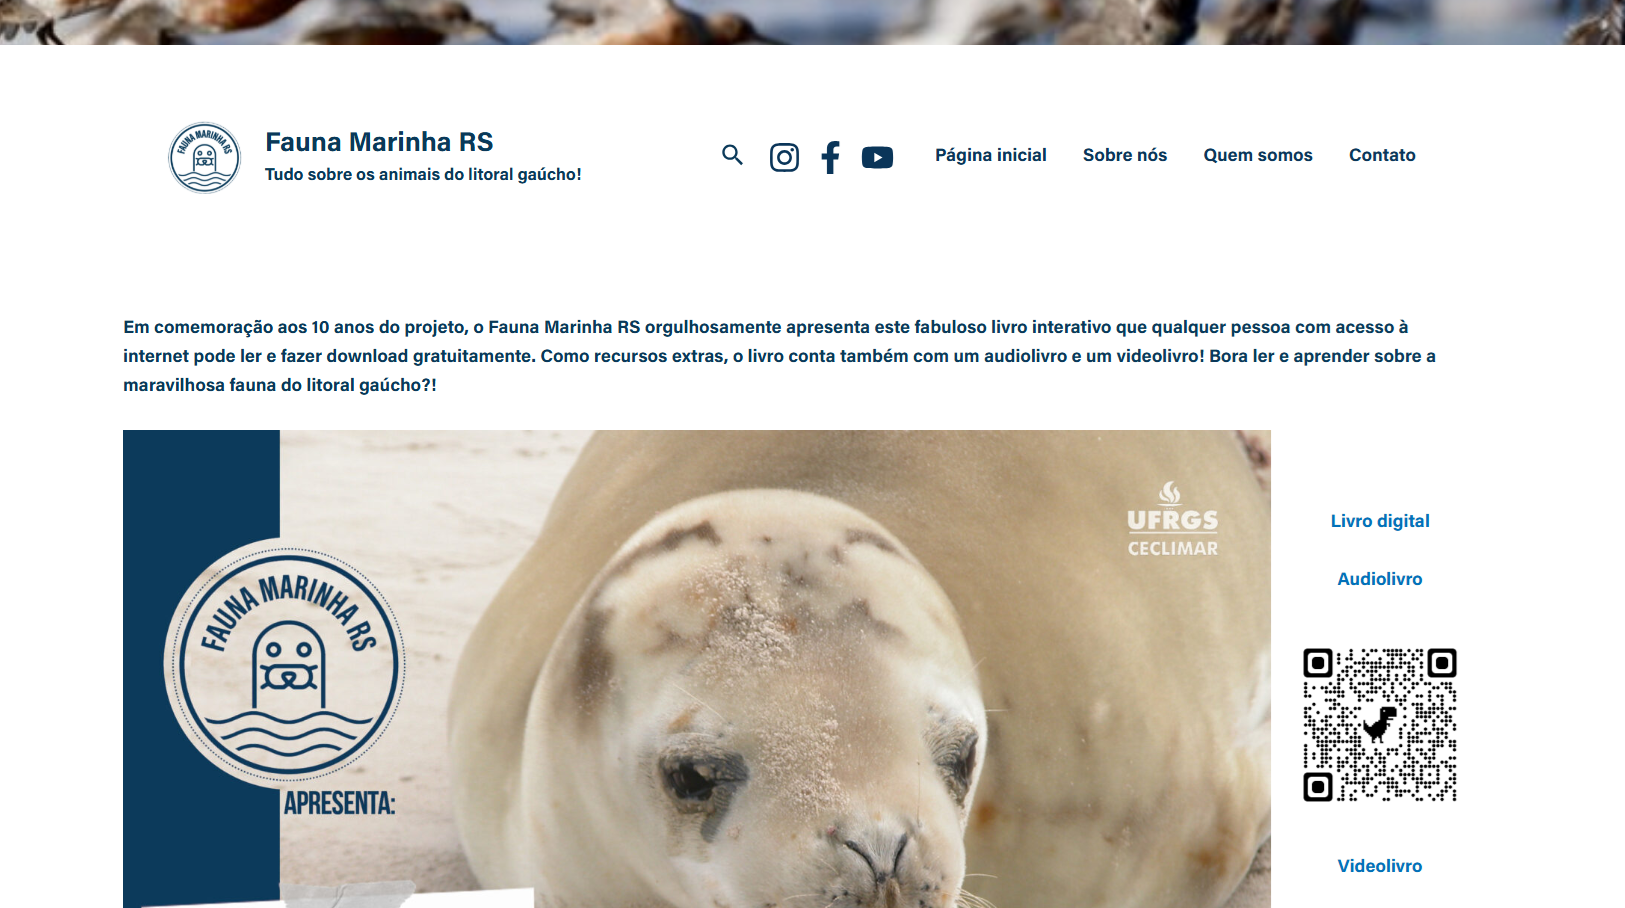
\includegraphics[width=1\textwidth]{imagens/sistemaWebFaunaMar.png}
    \caption{Identidade visual do sistema web do projeto Fauna Marinha RS.}
    \label{fig:identidade-visual-web}
\end{figure}
\legend{Fonte: \cite{faunamarinha2025}}

\begin{figure}[H]
    \centering
    
\includegraphics[height=0.5\textheight]{imagens/identidade-app.png}
    \caption{Identidade visual prototipada.}
    \label{fig:identidade-visual-mobile}
\end{figure}
\legend{Fonte: Autor}

\begin{figure}[H]
    \centering
    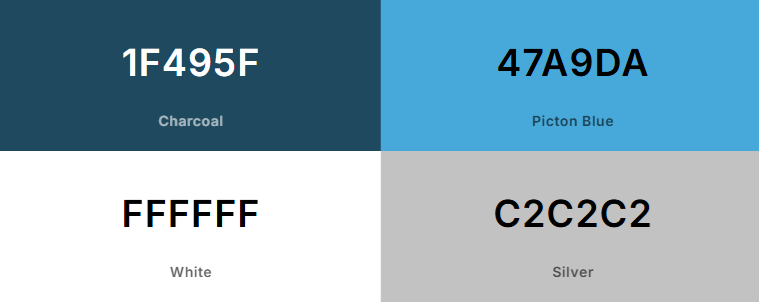
\includegraphics[width=1\textwidth]{imagens/paleta-cores.png}
    \caption{Paleta de cores utilizada.}
    \label{fig:paleta-cores}
\end{figure}
\legend{Fonte: Autor}

\subsection{Criação do Design das Telas}

Com base na identidade visual definida, foram elaborados os layouts das principais telas do 
aplicativo. Essa etapa concentrou-se na organização dos elementos de interface, na 
usabilidade e na experiência do usuário.

Inicialmente, foram criadas as telas de login (Figura~\ref{fig:prototipo-login}) e de 
registro de usuário (Figura~\ref{fig:prototipo-cadastro}).

\begin{figure}[H]
    \centering
    \begin{minipage}[b]{0.48\textwidth}
        \centering
        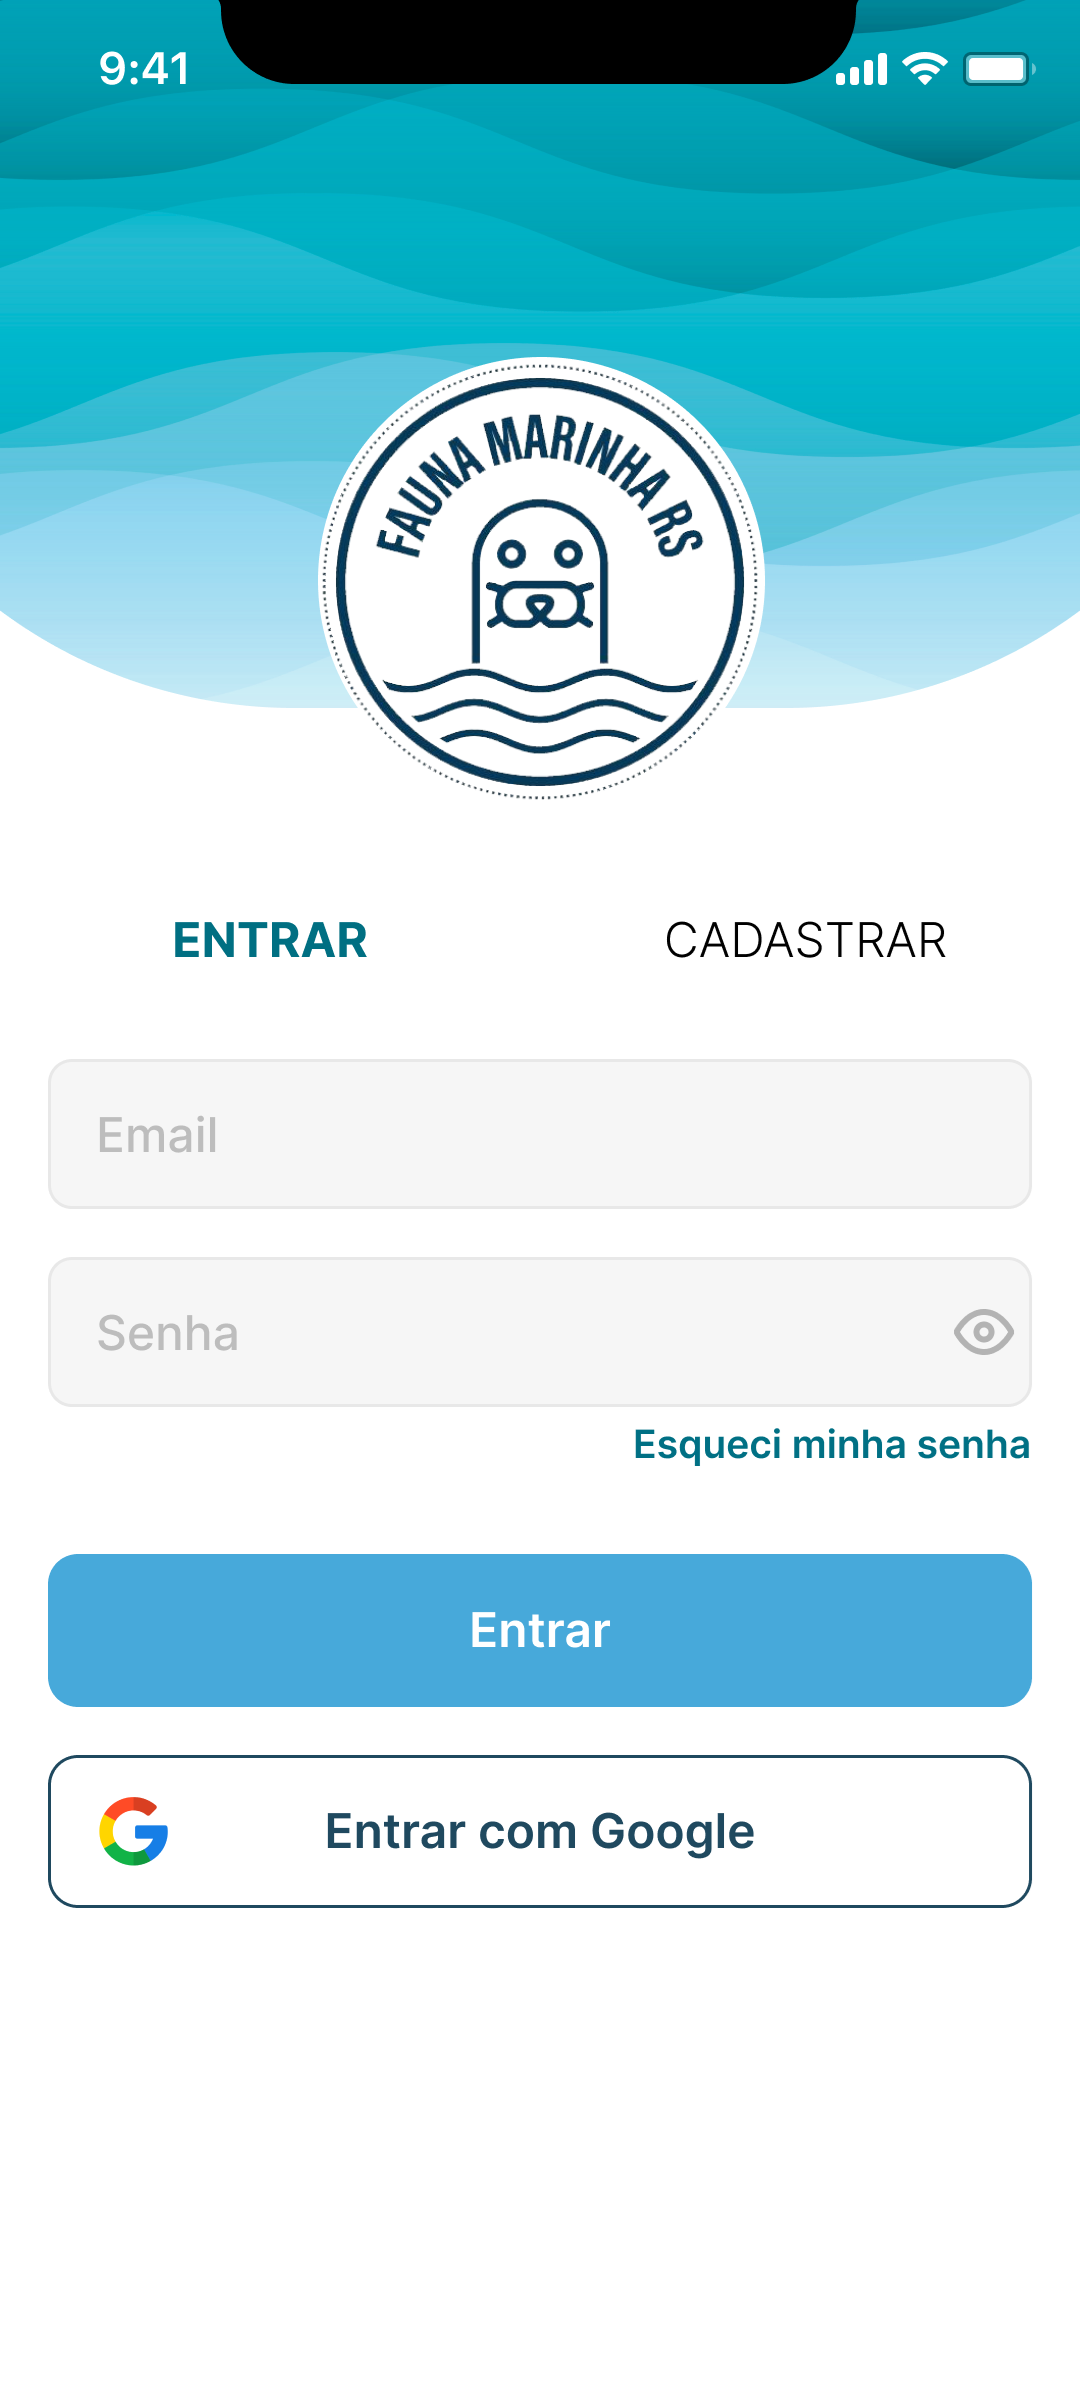
\includegraphics[height=0.6\textheight]{imagens/login-figma.png}
        \caption{Protótipo da tela de login do aplicativo.}
        \label{fig:prototipo-login}
    \end{minipage}
    \hfill
    \begin{minipage}[b]{0.48\textwidth}
        \centering
        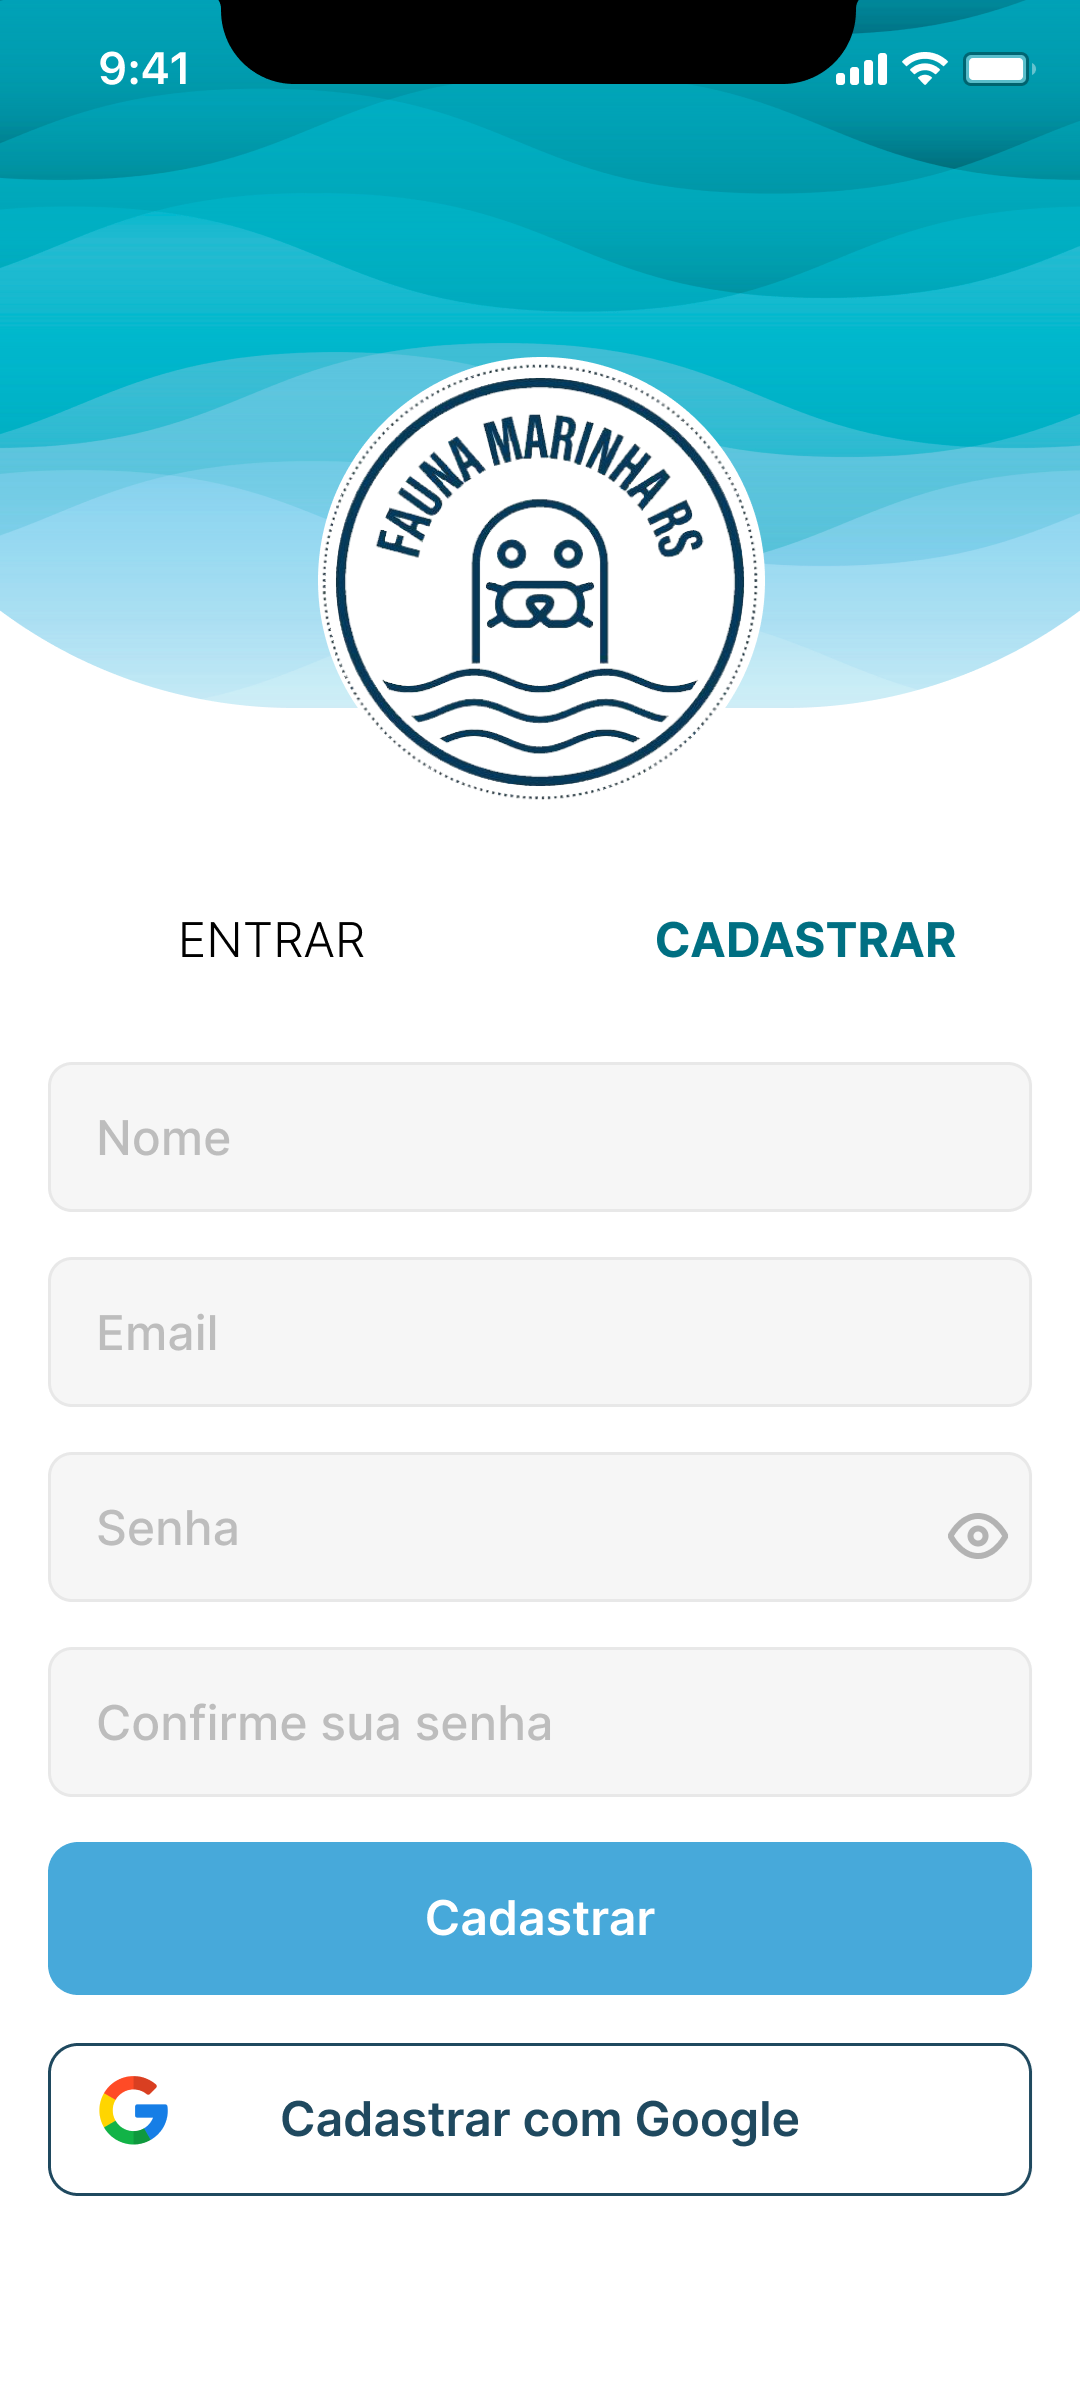
\includegraphics[height=0.6\textheight]{imagens/cadastro-figma.png}
        \caption{Protótipo da tela de cadastro do aplicativo.}
        \label{fig:prototipo-cadastro}
    \end{minipage}
\end{figure}
\legend{Fonte: Autor}

Em seguida, foi criada a tela inicial (Figura~\ref{fig:prototipo-home}), com duas 
variações: uma para usuários comuns e outra para pesquisadores. O layout foi pensado 
para facilitar o acesso às funcionalidades, com botões de acesso rápido e 
barra de navegação fixa na parte inferior da tela. A versão para pesquisadores apresenta os mesmos botões,
com a adição das funcionalidades exclusivas, avaliação de registros e acesso ao painel geral.

\begin{figure}[H]
    \centering
    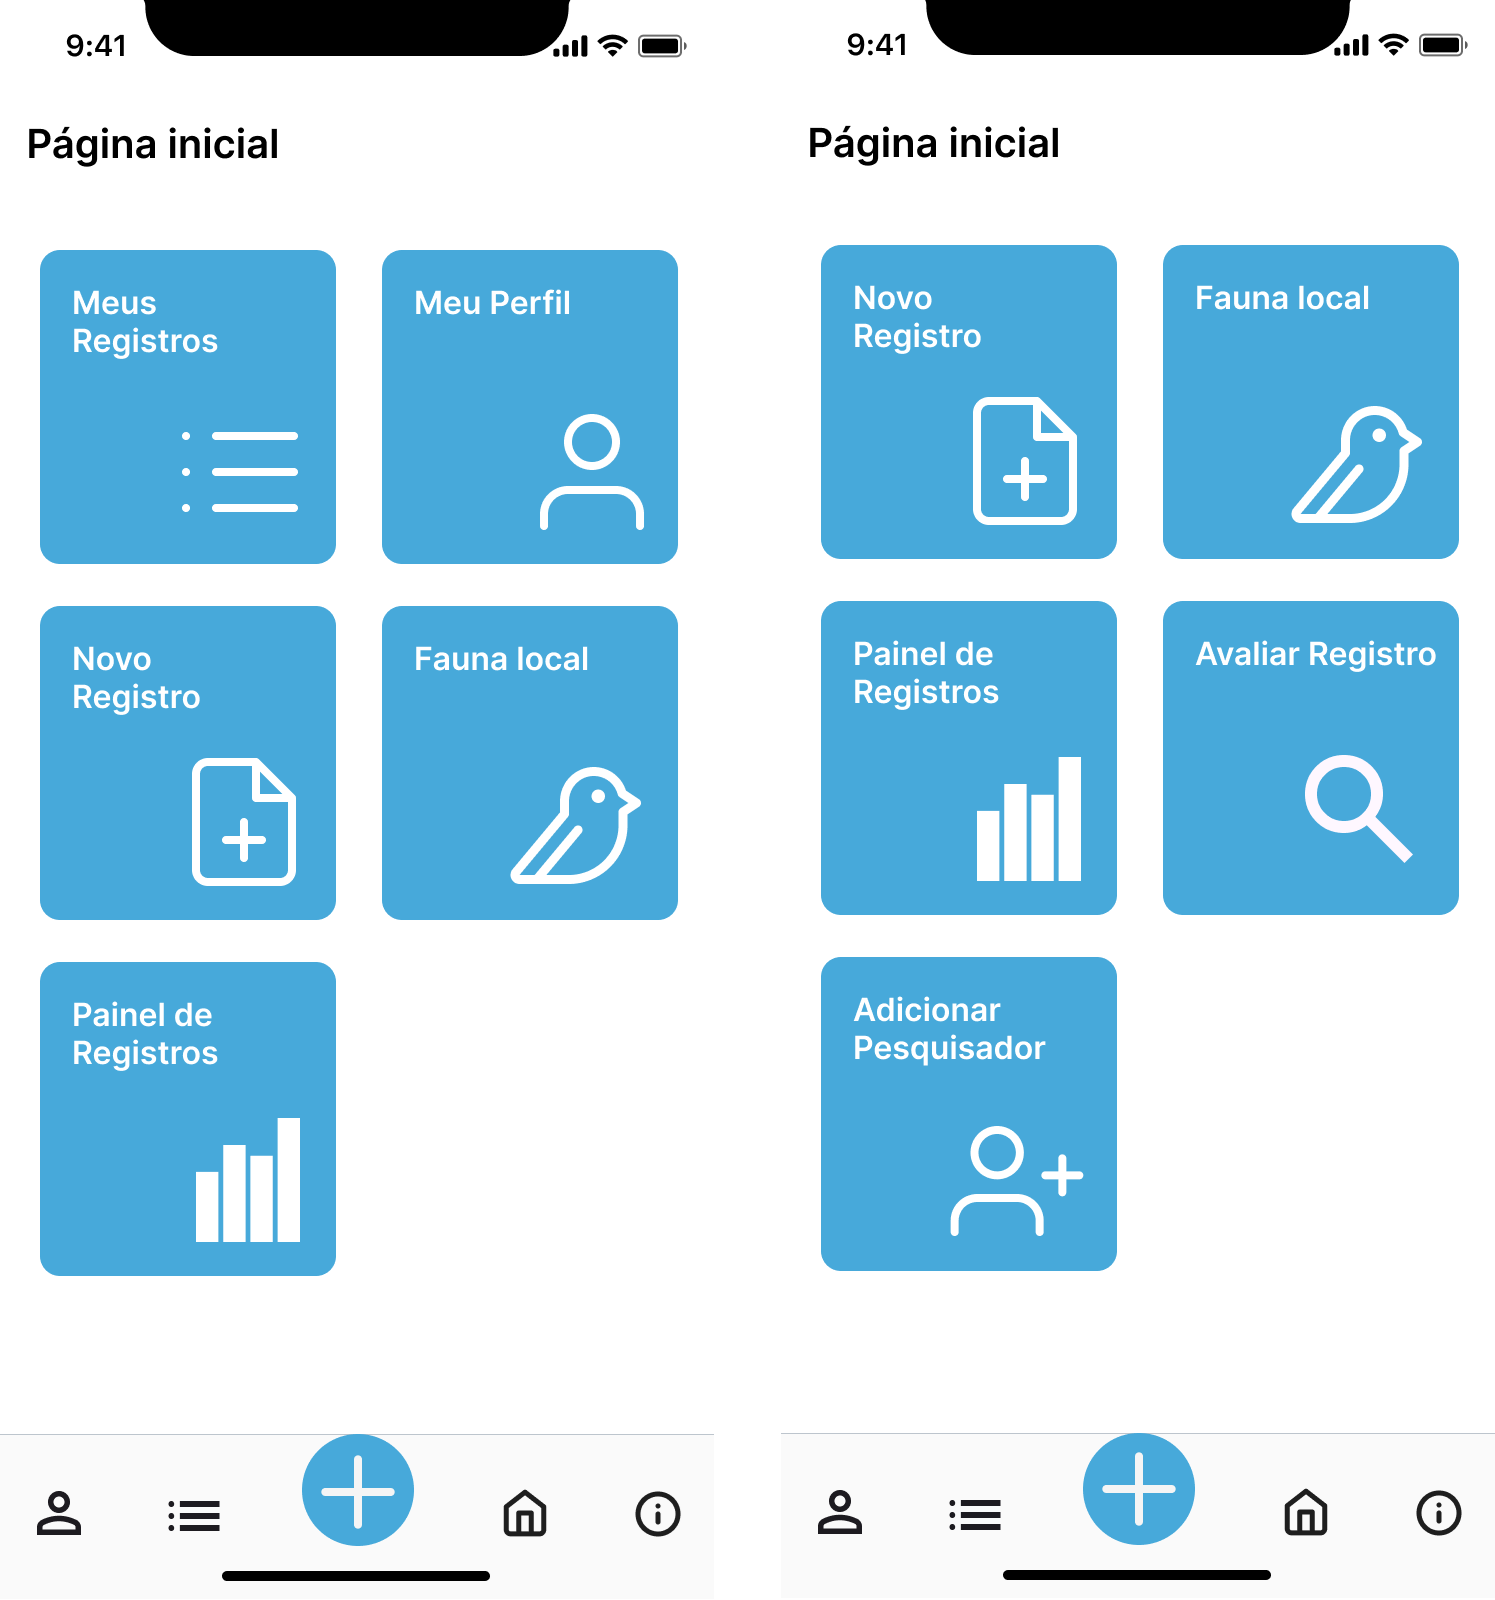
\includegraphics[height=0.6\textheight]{imagens/menu-pesquisador-figma.png}
    \caption{Protótipo da tela inicial: usuário comum (esquerda) e pesquisador (direita).}
    \label{fig:prototipo-home}
\end{figure}
\legend{Fonte: Autor}

A tela "Meus Registros" (Figura~\ref{fig:prototipo-meus-registros}) permite ao usuário 
visualizar todos os registros já enviados, com filtros por status (enviado e validado). 
Também foi projetado um estado com \textit{bottomsheet} acionado a partir do botão de adicionar 
registro ("+") na barra de navegação. Esse botão está disponível em qualquer tela, permitindo 
adicionar registros rapidamente.

\begin{figure}[H]
    \centering
    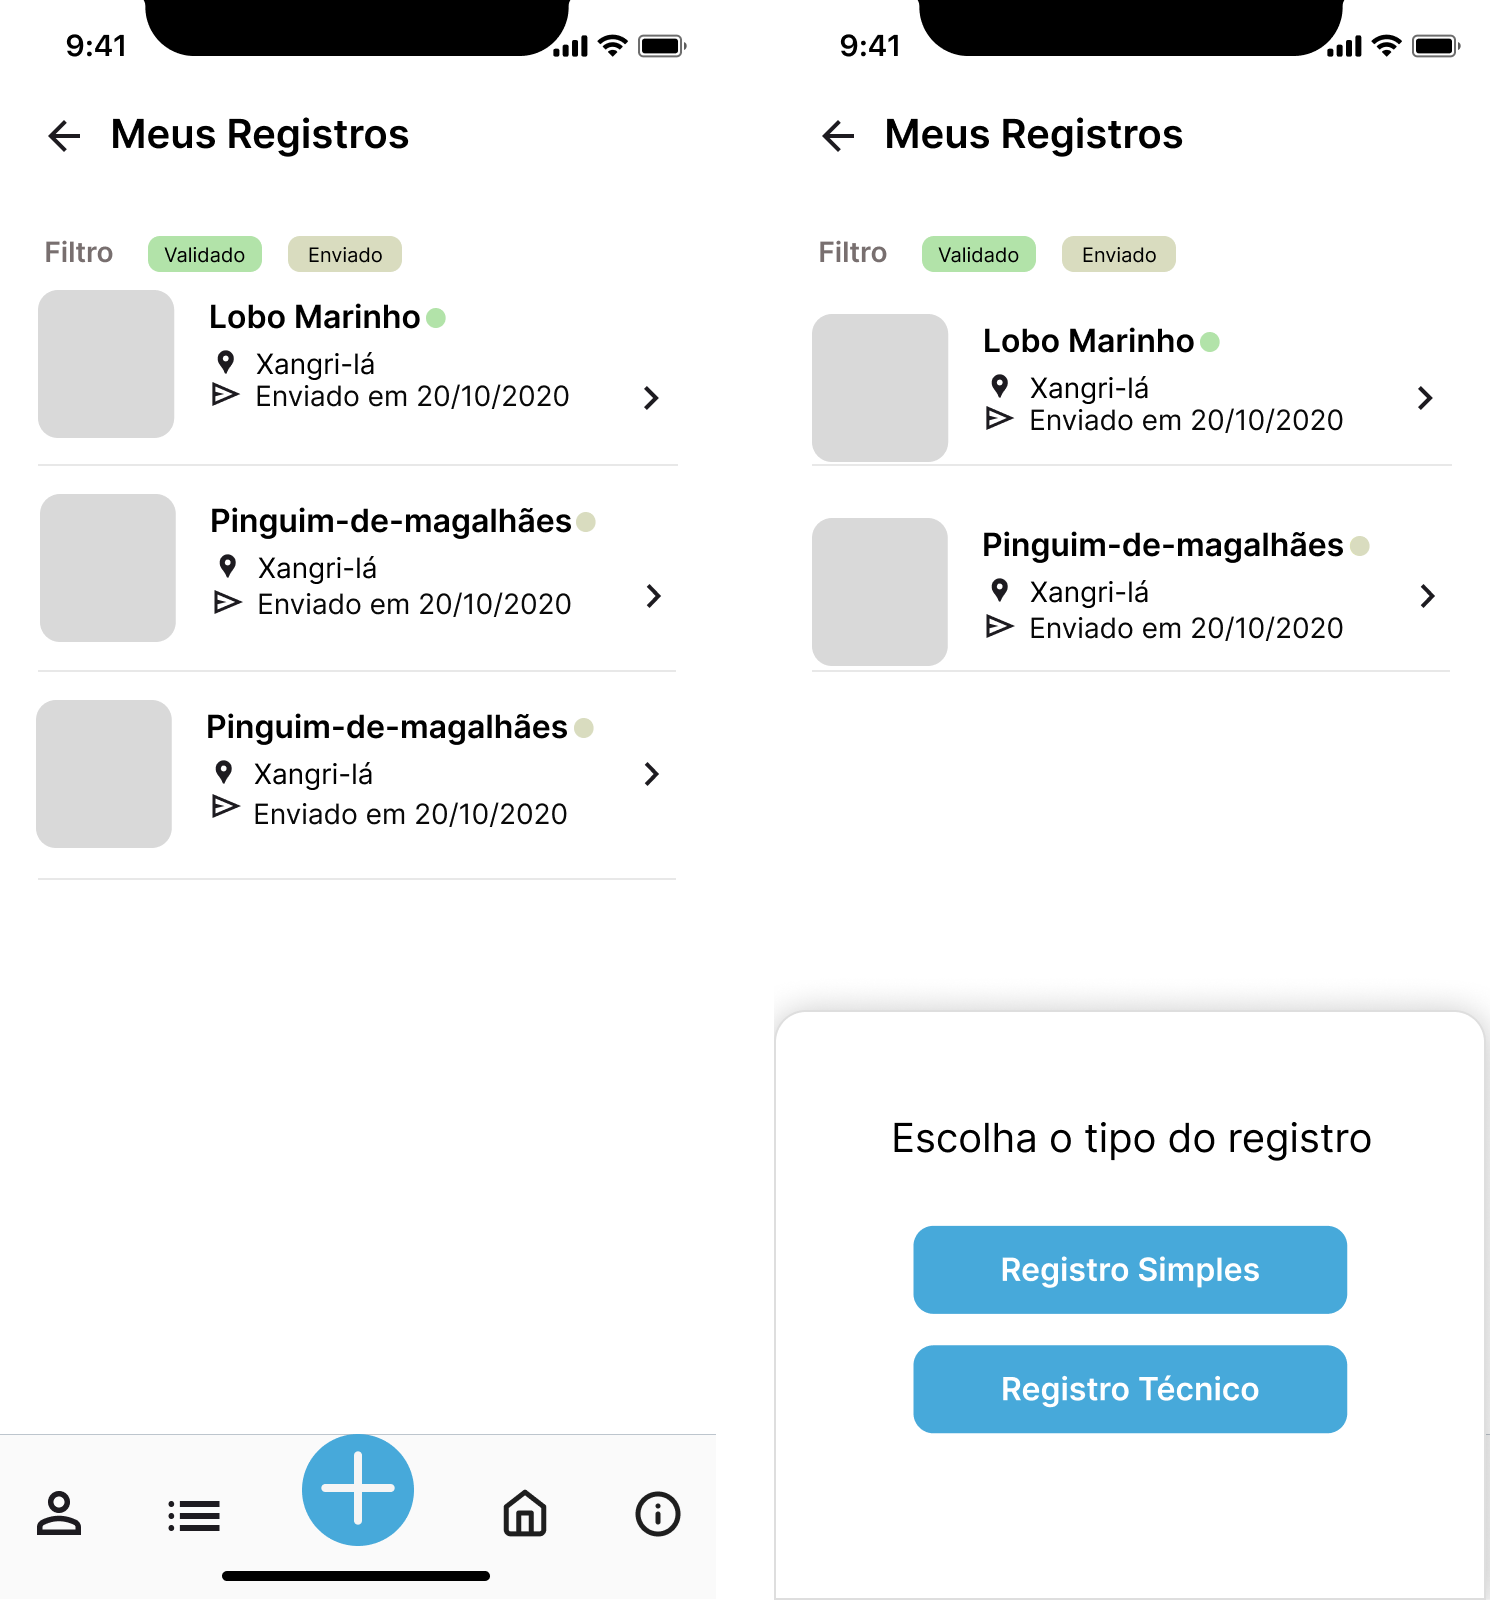
\includegraphics[height=0.6\textheight]{imagens/meus-registros-figma.png}
    \caption{Protótipo das telas de "Meus Registros" com estado ativo de adição de registro (direita).}
    \label{fig:prototipo-meus-registros}
\end{figure}
\legend{Fonte: Autor}

Dois tipos de formulários de registro foram projetados: um simples
 (Figura~\ref{fig:prototipo-registro-simples}), voltado a usuários leigos e envios rápidos, e 
 outro técnico (Figura~\ref{fig:prototipo-registro-tecnico}), com campos adicionais 
 para coleta de dados mais detalhados. Ambos possuem validações, campos obrigatórios e 
 opcionais, e suporte ao envio de imagens com orientações apresentadas em \textit{bottomsheet}.

Os campos específicos de classe, ordem, família e gênero foram projetados para serem um dropdown,
que apresentará as opções disponíveis para o usuário selecionar.

\begin{figure}[H]
    \centering
    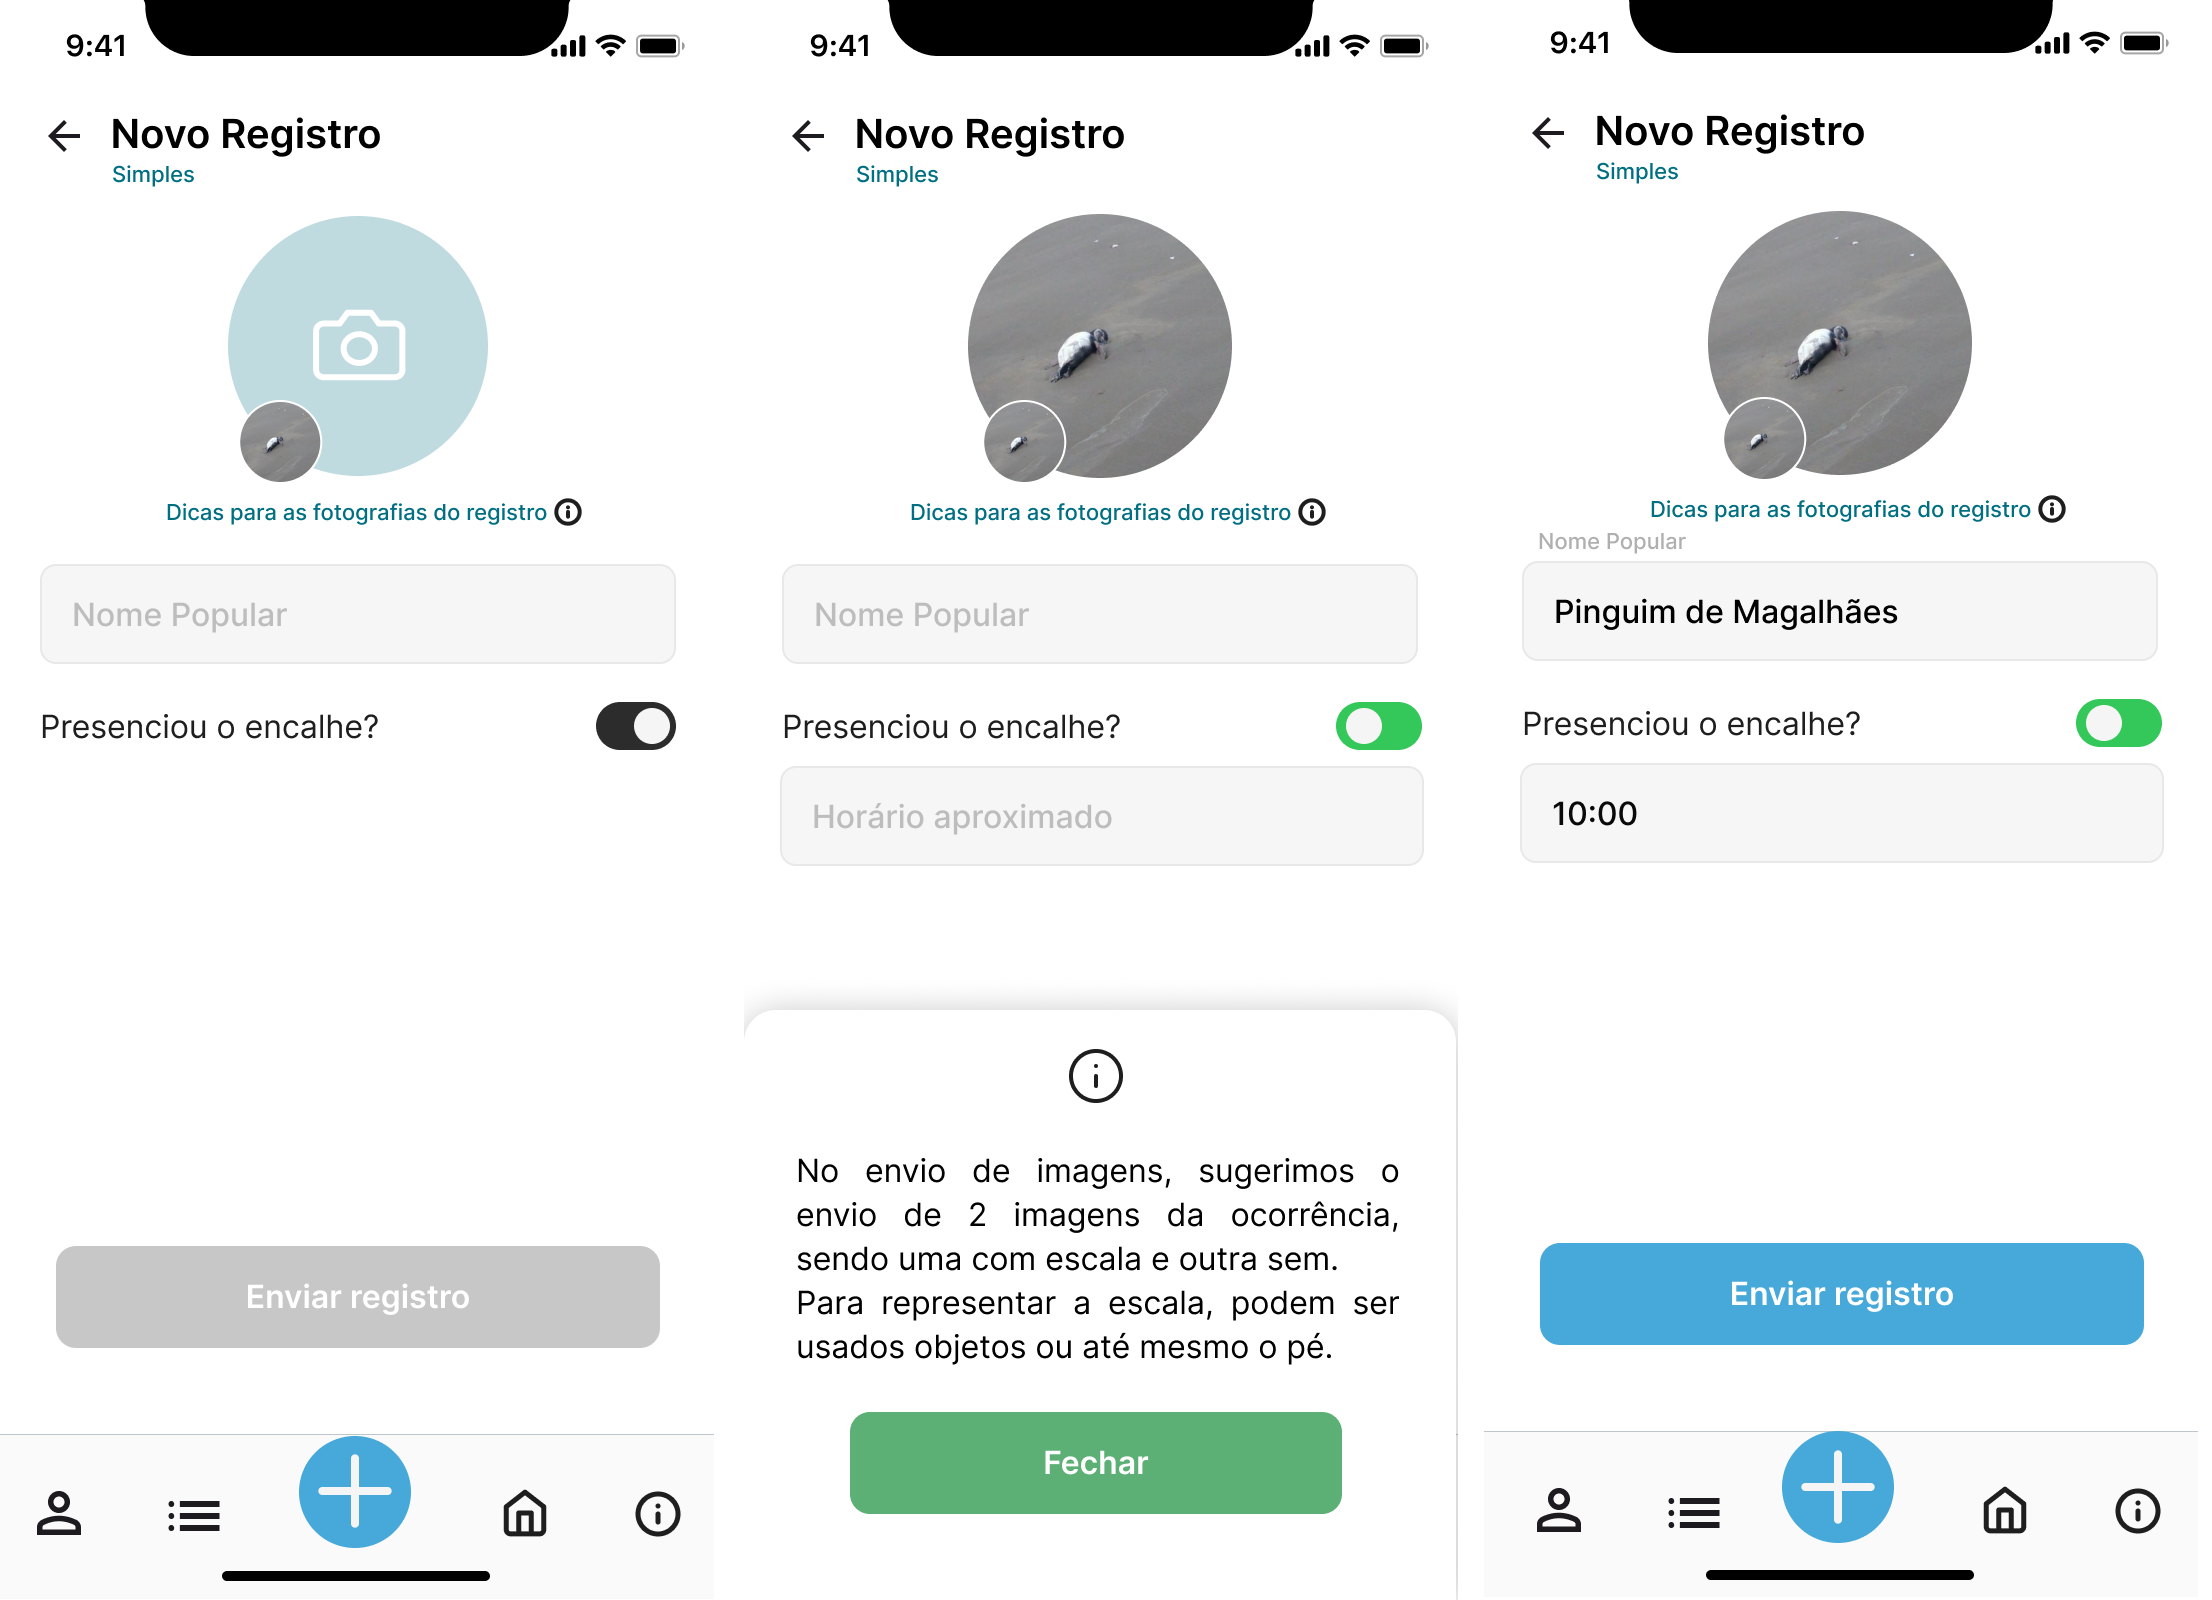
\includegraphics[height=0.55\textheight, width=\textwidth]{imagens/registro-simples-figma.png}
    \caption{Protótipo do formulário de registro simples. Centro: \textit{bottomsheet} informativa; direita: campo 
    adicional ativado.}
    \label{fig:prototipo-registro-simples}
\end{figure}
\legend{Fonte: Autor}

\begin{figure}[H]
    \centering
    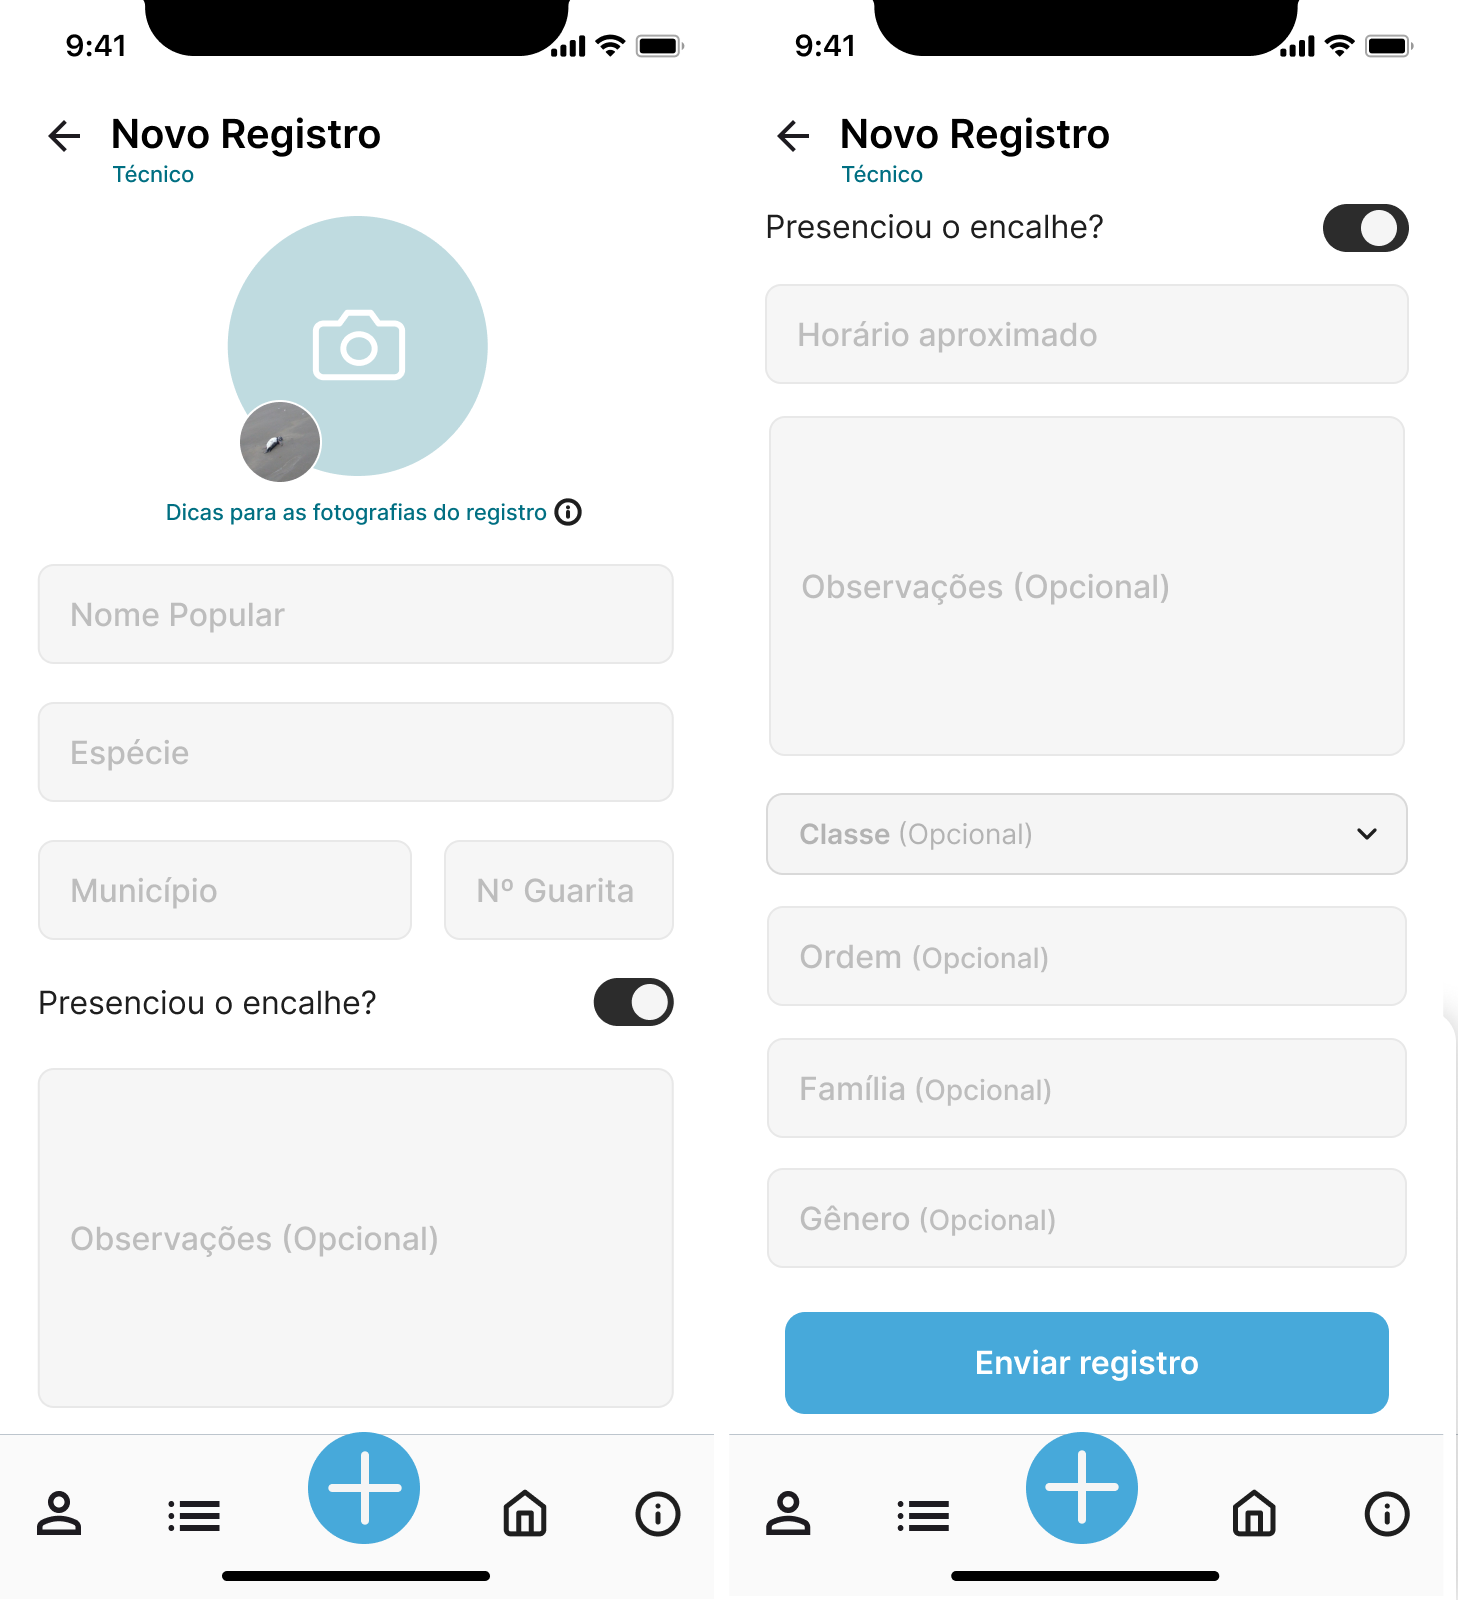
\includegraphics[height=0.6\textheight]{imagens/registro-tecnico-figma.png}
    \caption{Protótipo do formulário de registro técnico com campos taxonômicos e detalhamento avançado.}
    \label{fig:prototipo-registro-tecnico}
\end{figure}
\legend{Fonte: Autor}

A tela de "Registros Pendentes" (Figura~\ref{fig:prototipo-registros-pendentes}) foi projetada 
para uso exclusivo de pesquisadores, permitindo acesso aos registros ainda não avaliados enviados 
por todos os usuários.

\begin{figure}[H]
    \centering
    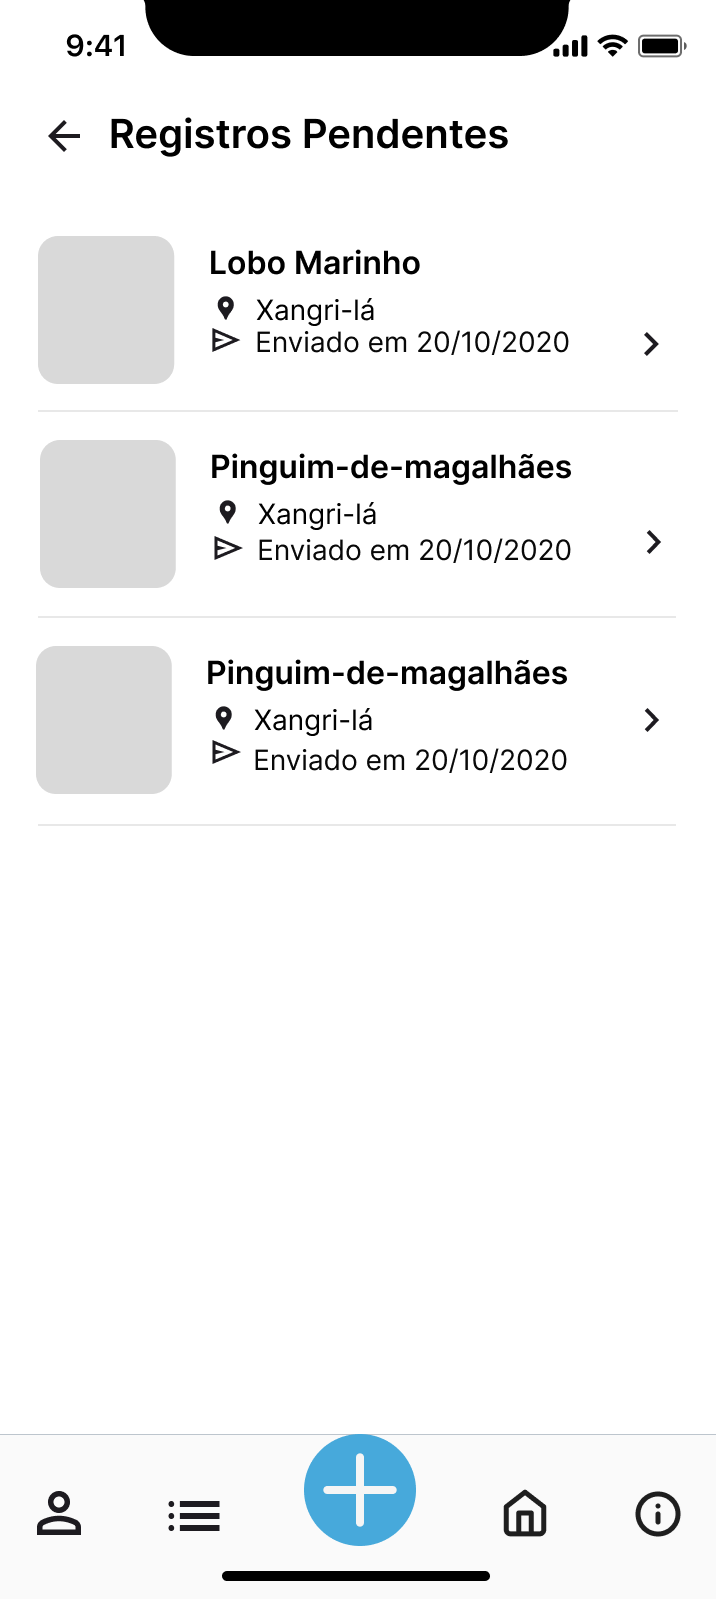
\includegraphics[height=0.6\textheight]{imagens/registro-pendente-figma.png}
    \caption{Protótipo da tela de registros pendentes, acessível apenas a pesquisadores.}
    \label{fig:prototipo-registros-pendentes}
\end{figure}
\legend{Fonte: Autor}

A tela de "Analisar Registro" (Figura~\ref{fig:prototipo-avaliar-registro}) foi projetada para 
permitir que o pesquisador visualize os dados enviados em cada registro 
com a possibilidade de editar os dados, adicionar comentários e enviar uma atualização o registro.
Se fez importante adicionar um estado para esta tela, onde o pesquisador consiga selecionar a imagem
para uma visualização em tela cheia, facilitando a análise do registro.

\begin{figure}[H]
    \centering
    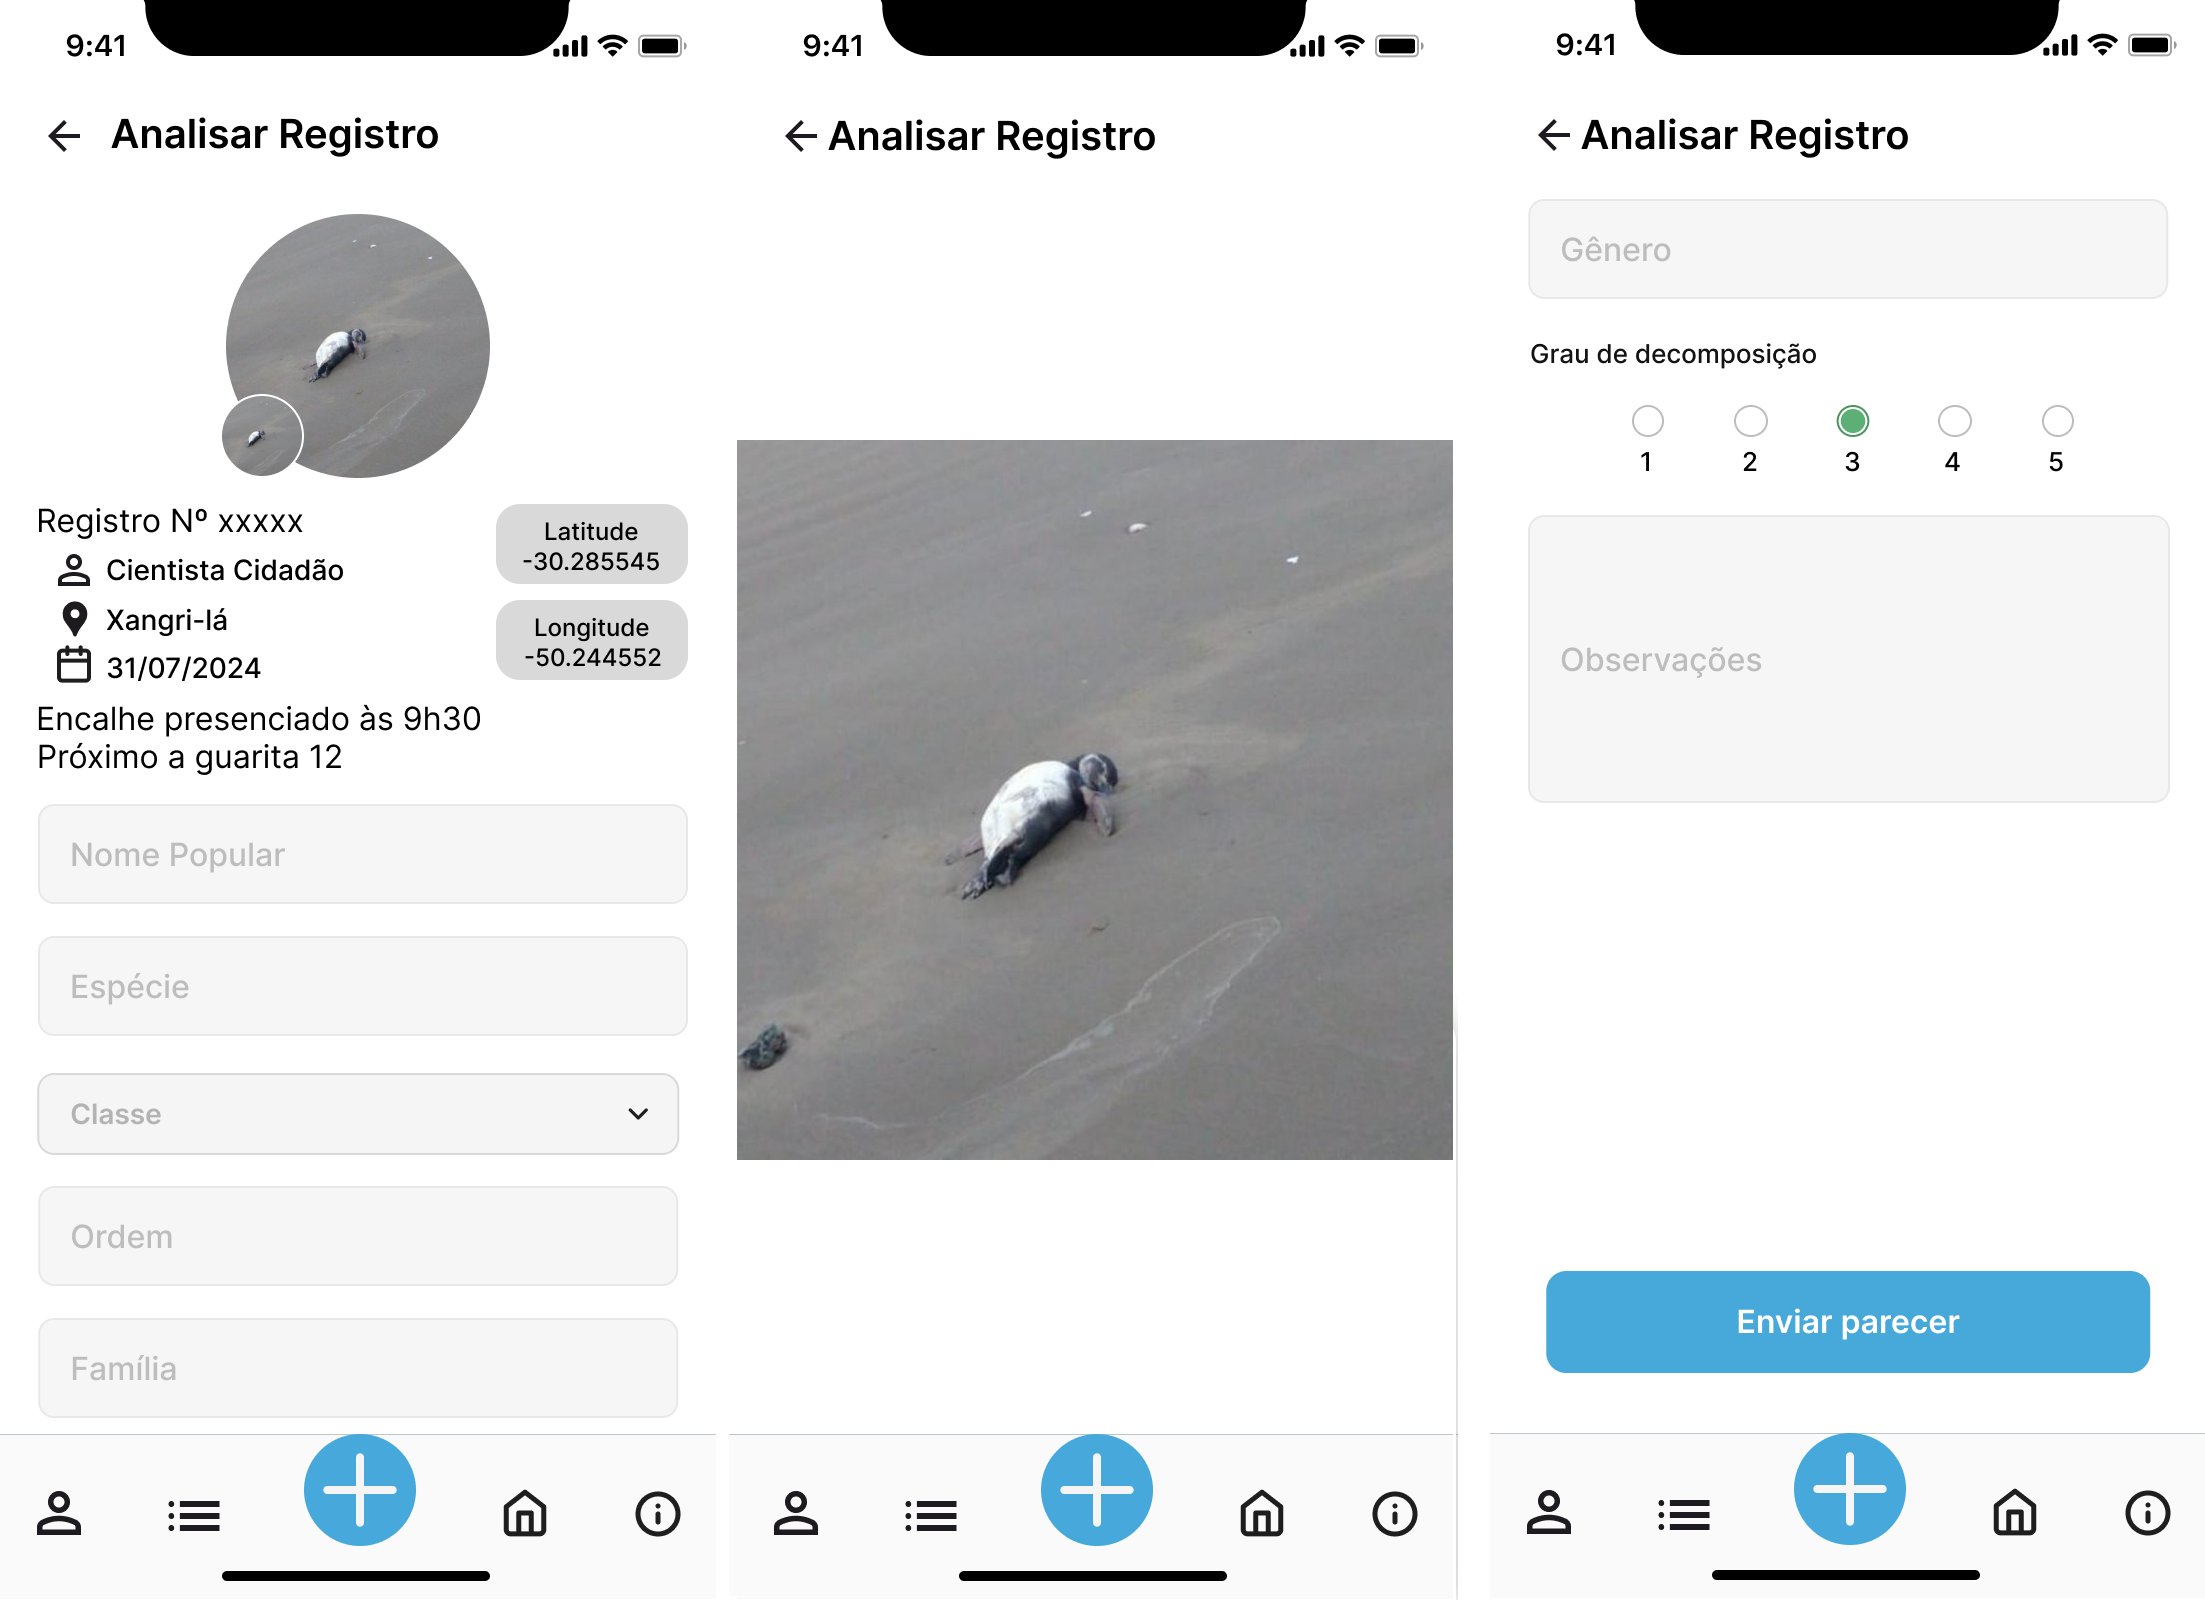
\includegraphics[height=0.55\textheight, width=\textwidth]{imagens/avaliar-registro-figma.png}
    \caption{Protótipo da tela de análise de registro. Ao centro, visualização ampliada da imagem.}
    \label{fig:prototipo-avaliar-registro}
\end{figure}
\legend{Fonte: Autor}

A tela de "Visualizar Registro" foi projetada para permitir que o usuário visualize os dados
enviados e validados. Para os dados já foram validados 
(Figura~\ref{fig:prototipo-ver-registro-validado}), o registro apresentará dados extras 
sobre aquele registro, como grau de decomposição, parecer do profissional e taxonomia avaliada.
Já para os dados que ainda não foram validados (Figura~\ref{fig:prototipo-ver-registro-enviado}), 
o usuário verá apenas as informações que ele mesmo enviou.

\begin{figure}[H]
    \centering
    \begin{minipage}[b]{0.48\textwidth}
        \centering
        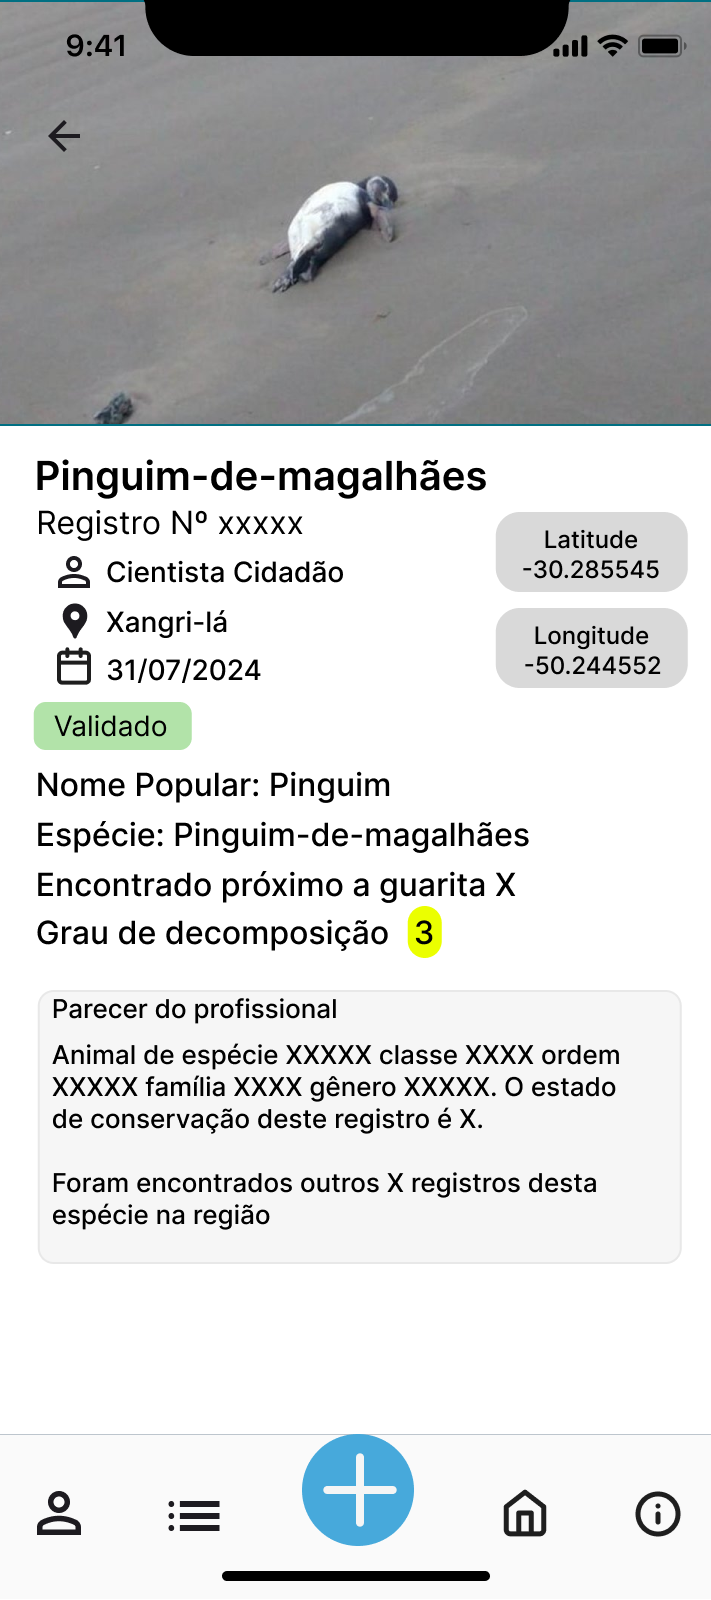
\includegraphics[height=0.6\textheight]{imagens/ver-registro-figma.png}
        \caption{Protótipo da visualização de registro validado.}
        \label{fig:prototipo-ver-registro-validado}
    \end{minipage}
    \hfill
    \begin{minipage}[b]{0.48\textwidth}
        \centering
        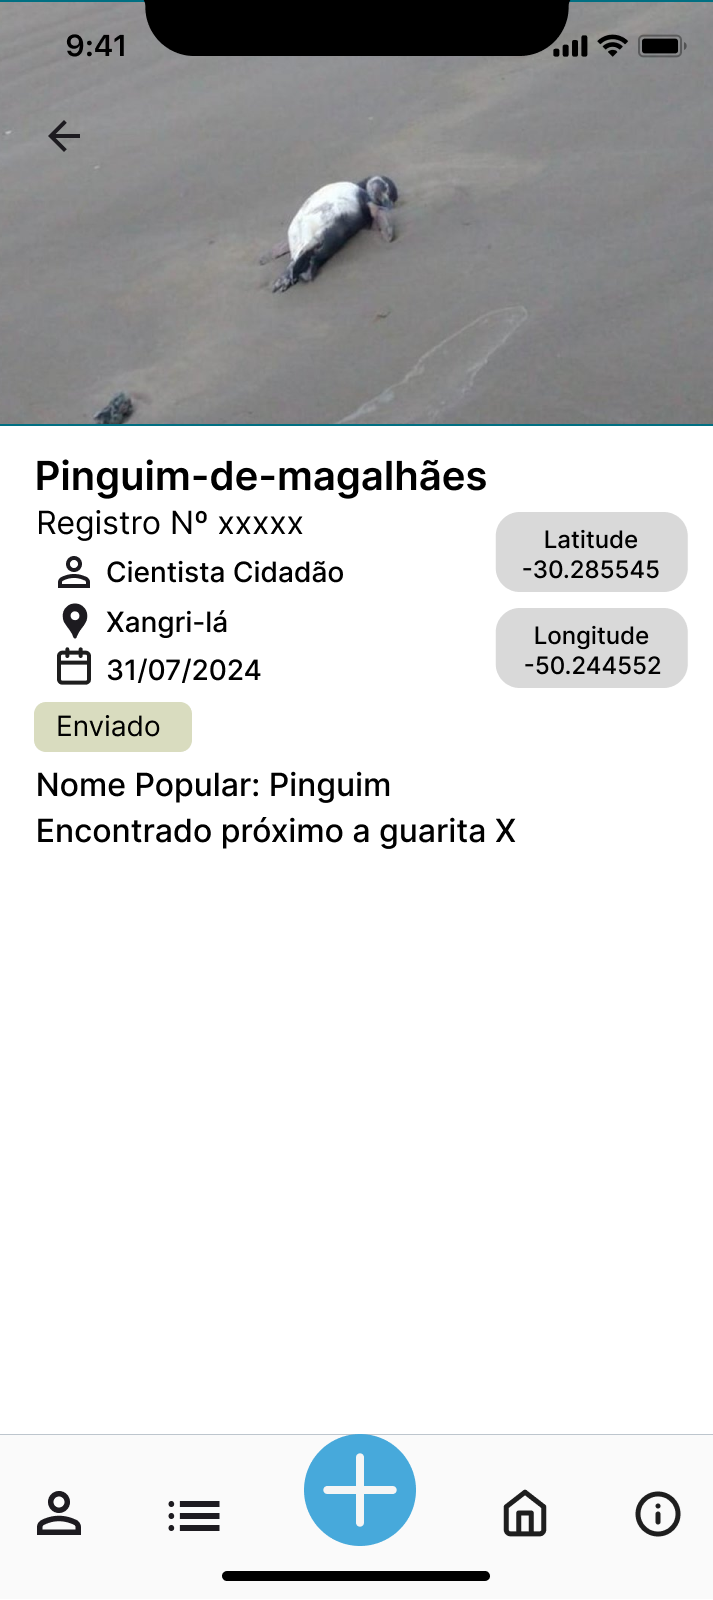
\includegraphics[height=0.6\textheight]{imagens/ve-registro-enviado-figma.png}
        \caption{Protótipo da visualização de registro enviado, ainda não avaliado.}
        \label{fig:prototipo-ver-registro-enviado}
    \end{minipage}
\end{figure}
\legend{Fonte: Autor}

A tela de perfil do usuário (Figura~\ref{fig:prototipo-perfil}) apresenta dados básicos, 
quantidade de registros enviados, últimos registros e conquistas. As conquistas são exibidas 
em formato de medalhas organizadas em uma grade com três colunas.

\begin{figure}[H]
    \centering
    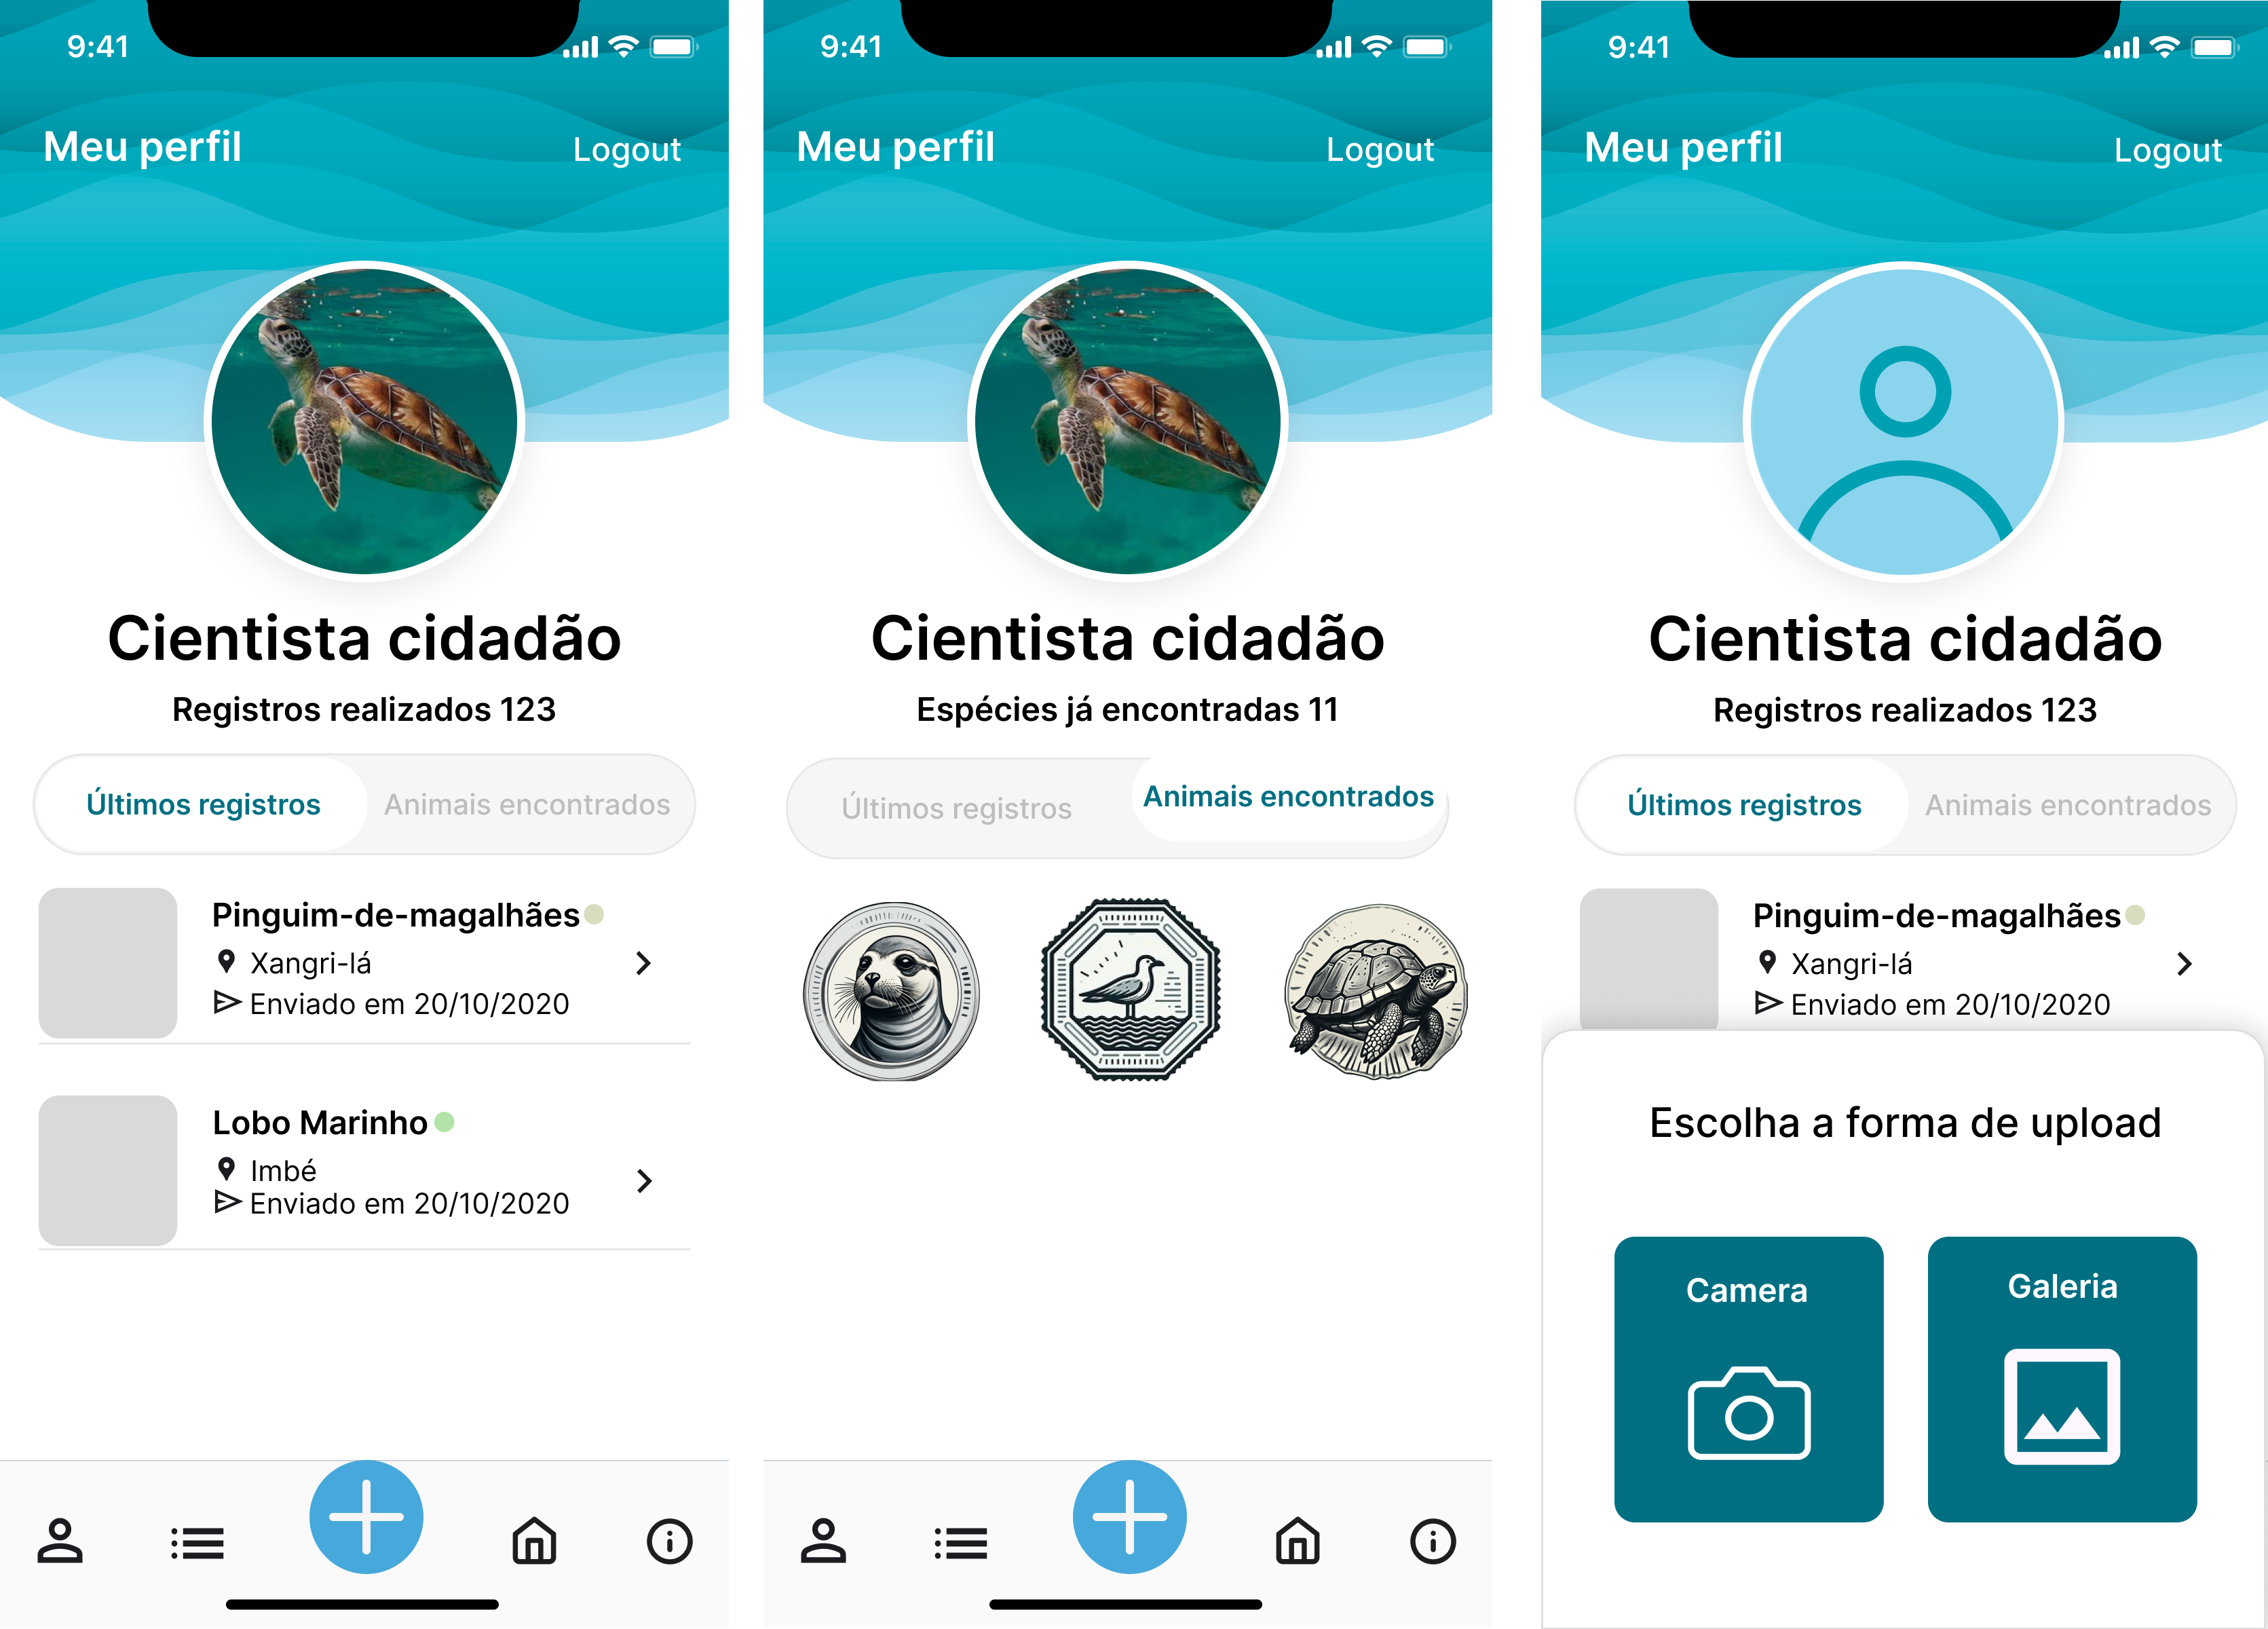
\includegraphics[height=0.53\textheight, width=\textwidth]{imagens/perfil-figma.png}
    \caption{Protótipo da tela de perfil do usuário com conquistas e histórico.}
    \label{fig:prototipo-perfil}
\end{figure}
\legend{Fonte: Autor}

As telas de fauna local (Figura~\ref{fig:prototipo-fauna-local}) seguem o mesmo padrão visual 
das demais telas do aplicativo, se assemelhando em estrutura com a de "Meus Registros" e 
"Visualizar Registro". Elas apresentam, respectivamente, uma lista de espécies e uma 
tela de detalhes com informações específicas sobre cada animal que for selecionado.

\begin{figure}[H]
    \centering
    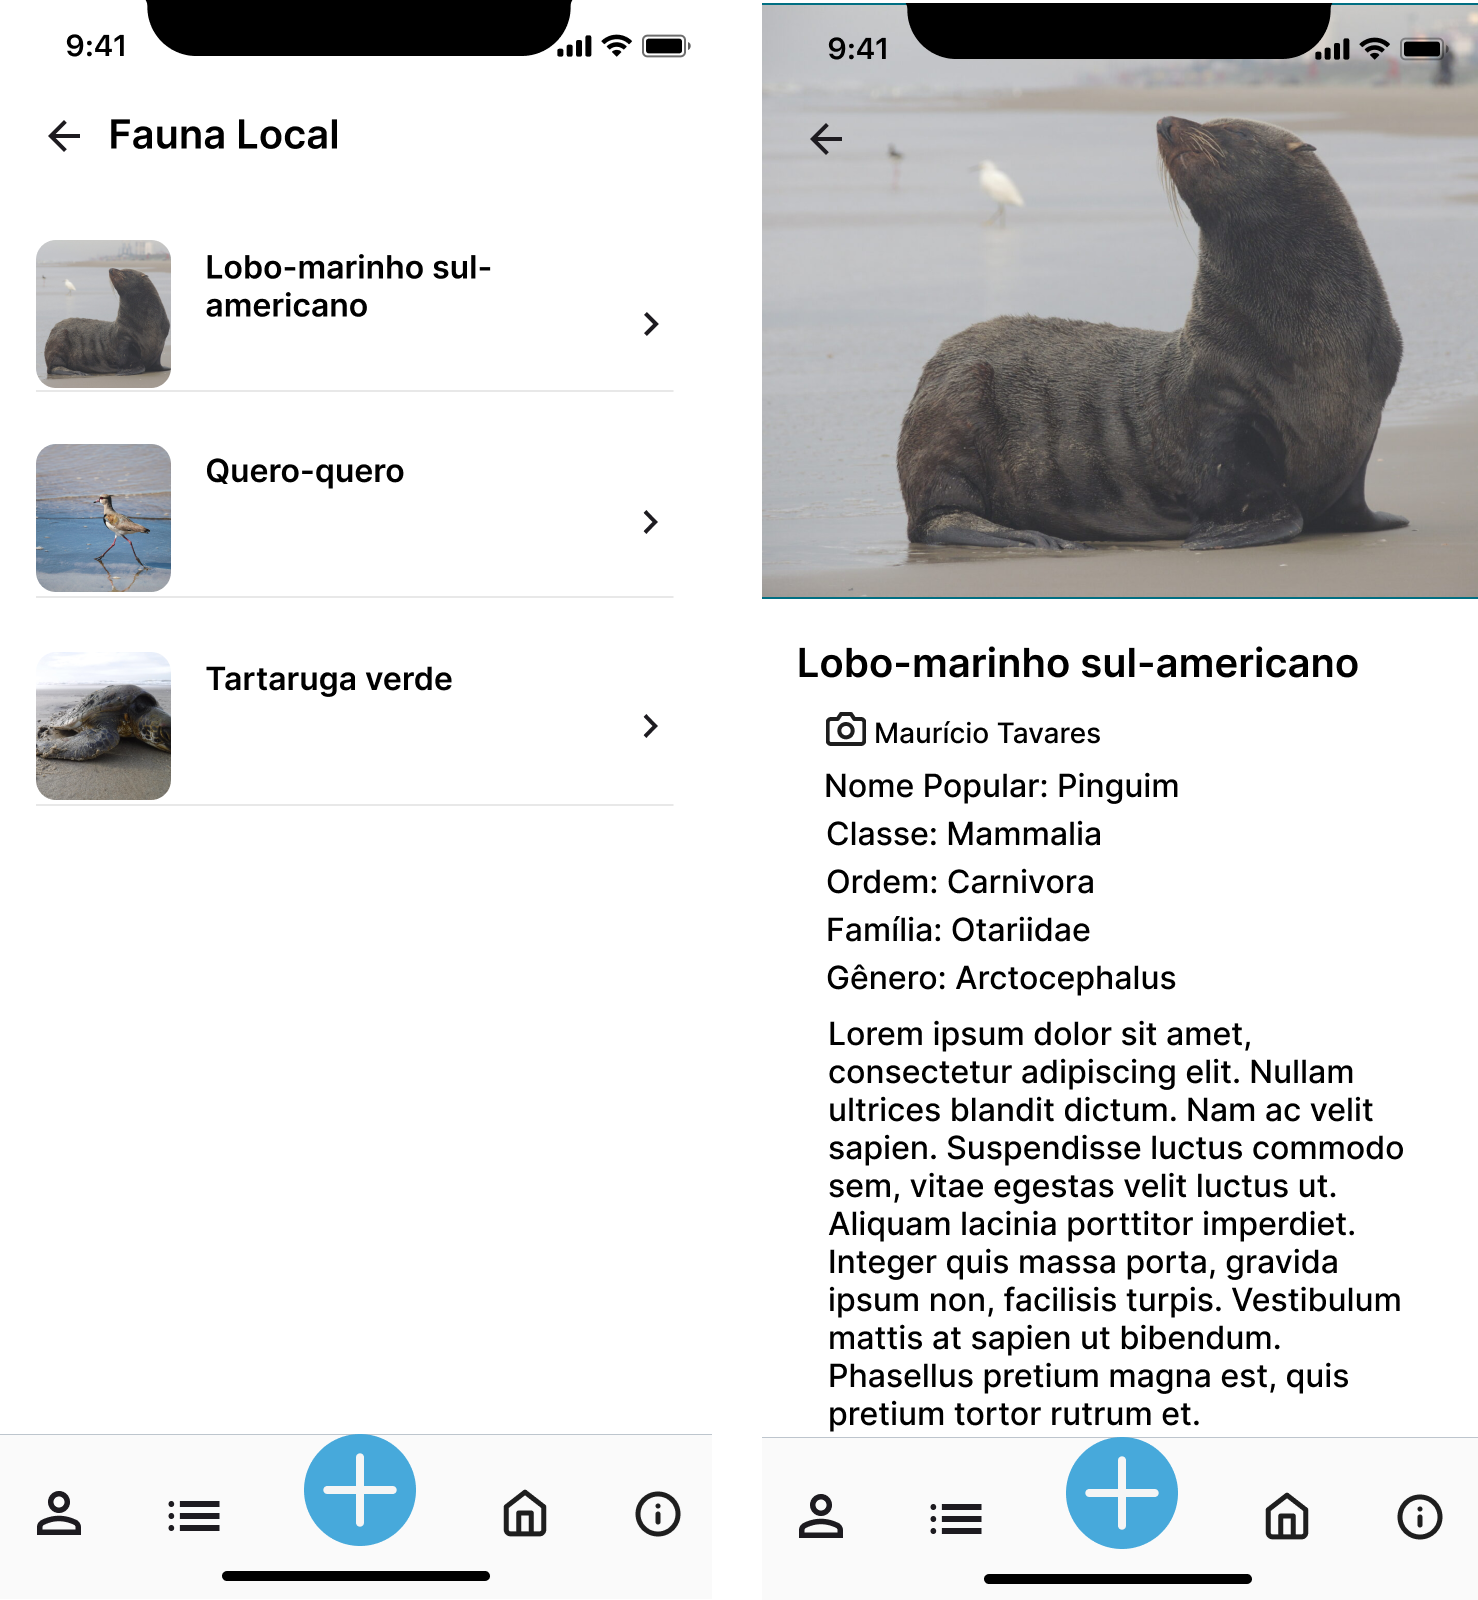
\includegraphics[height=0.6\textheight]{imagens/fauna-local-figma.png}
    \caption{Protótipo da tela de fauna local (esquerda) e detalhes da espécie (direita).}
    \label{fig:prototipo-fauna-local}
\end{figure}
\legend{Fonte: Autor}

Por fim, foi projetada a tela de recuperação de senha (Figura~\ref{fig:prototipo-esqueci-senha}), 
incluindo os estados de sucesso e de erro na validação dos campos de entrada. O padrão de erro 
apresentado nesta tela foi o mesmo utilizado em outras telas do aplicativo.

\begin{figure}[H]
    \centering
    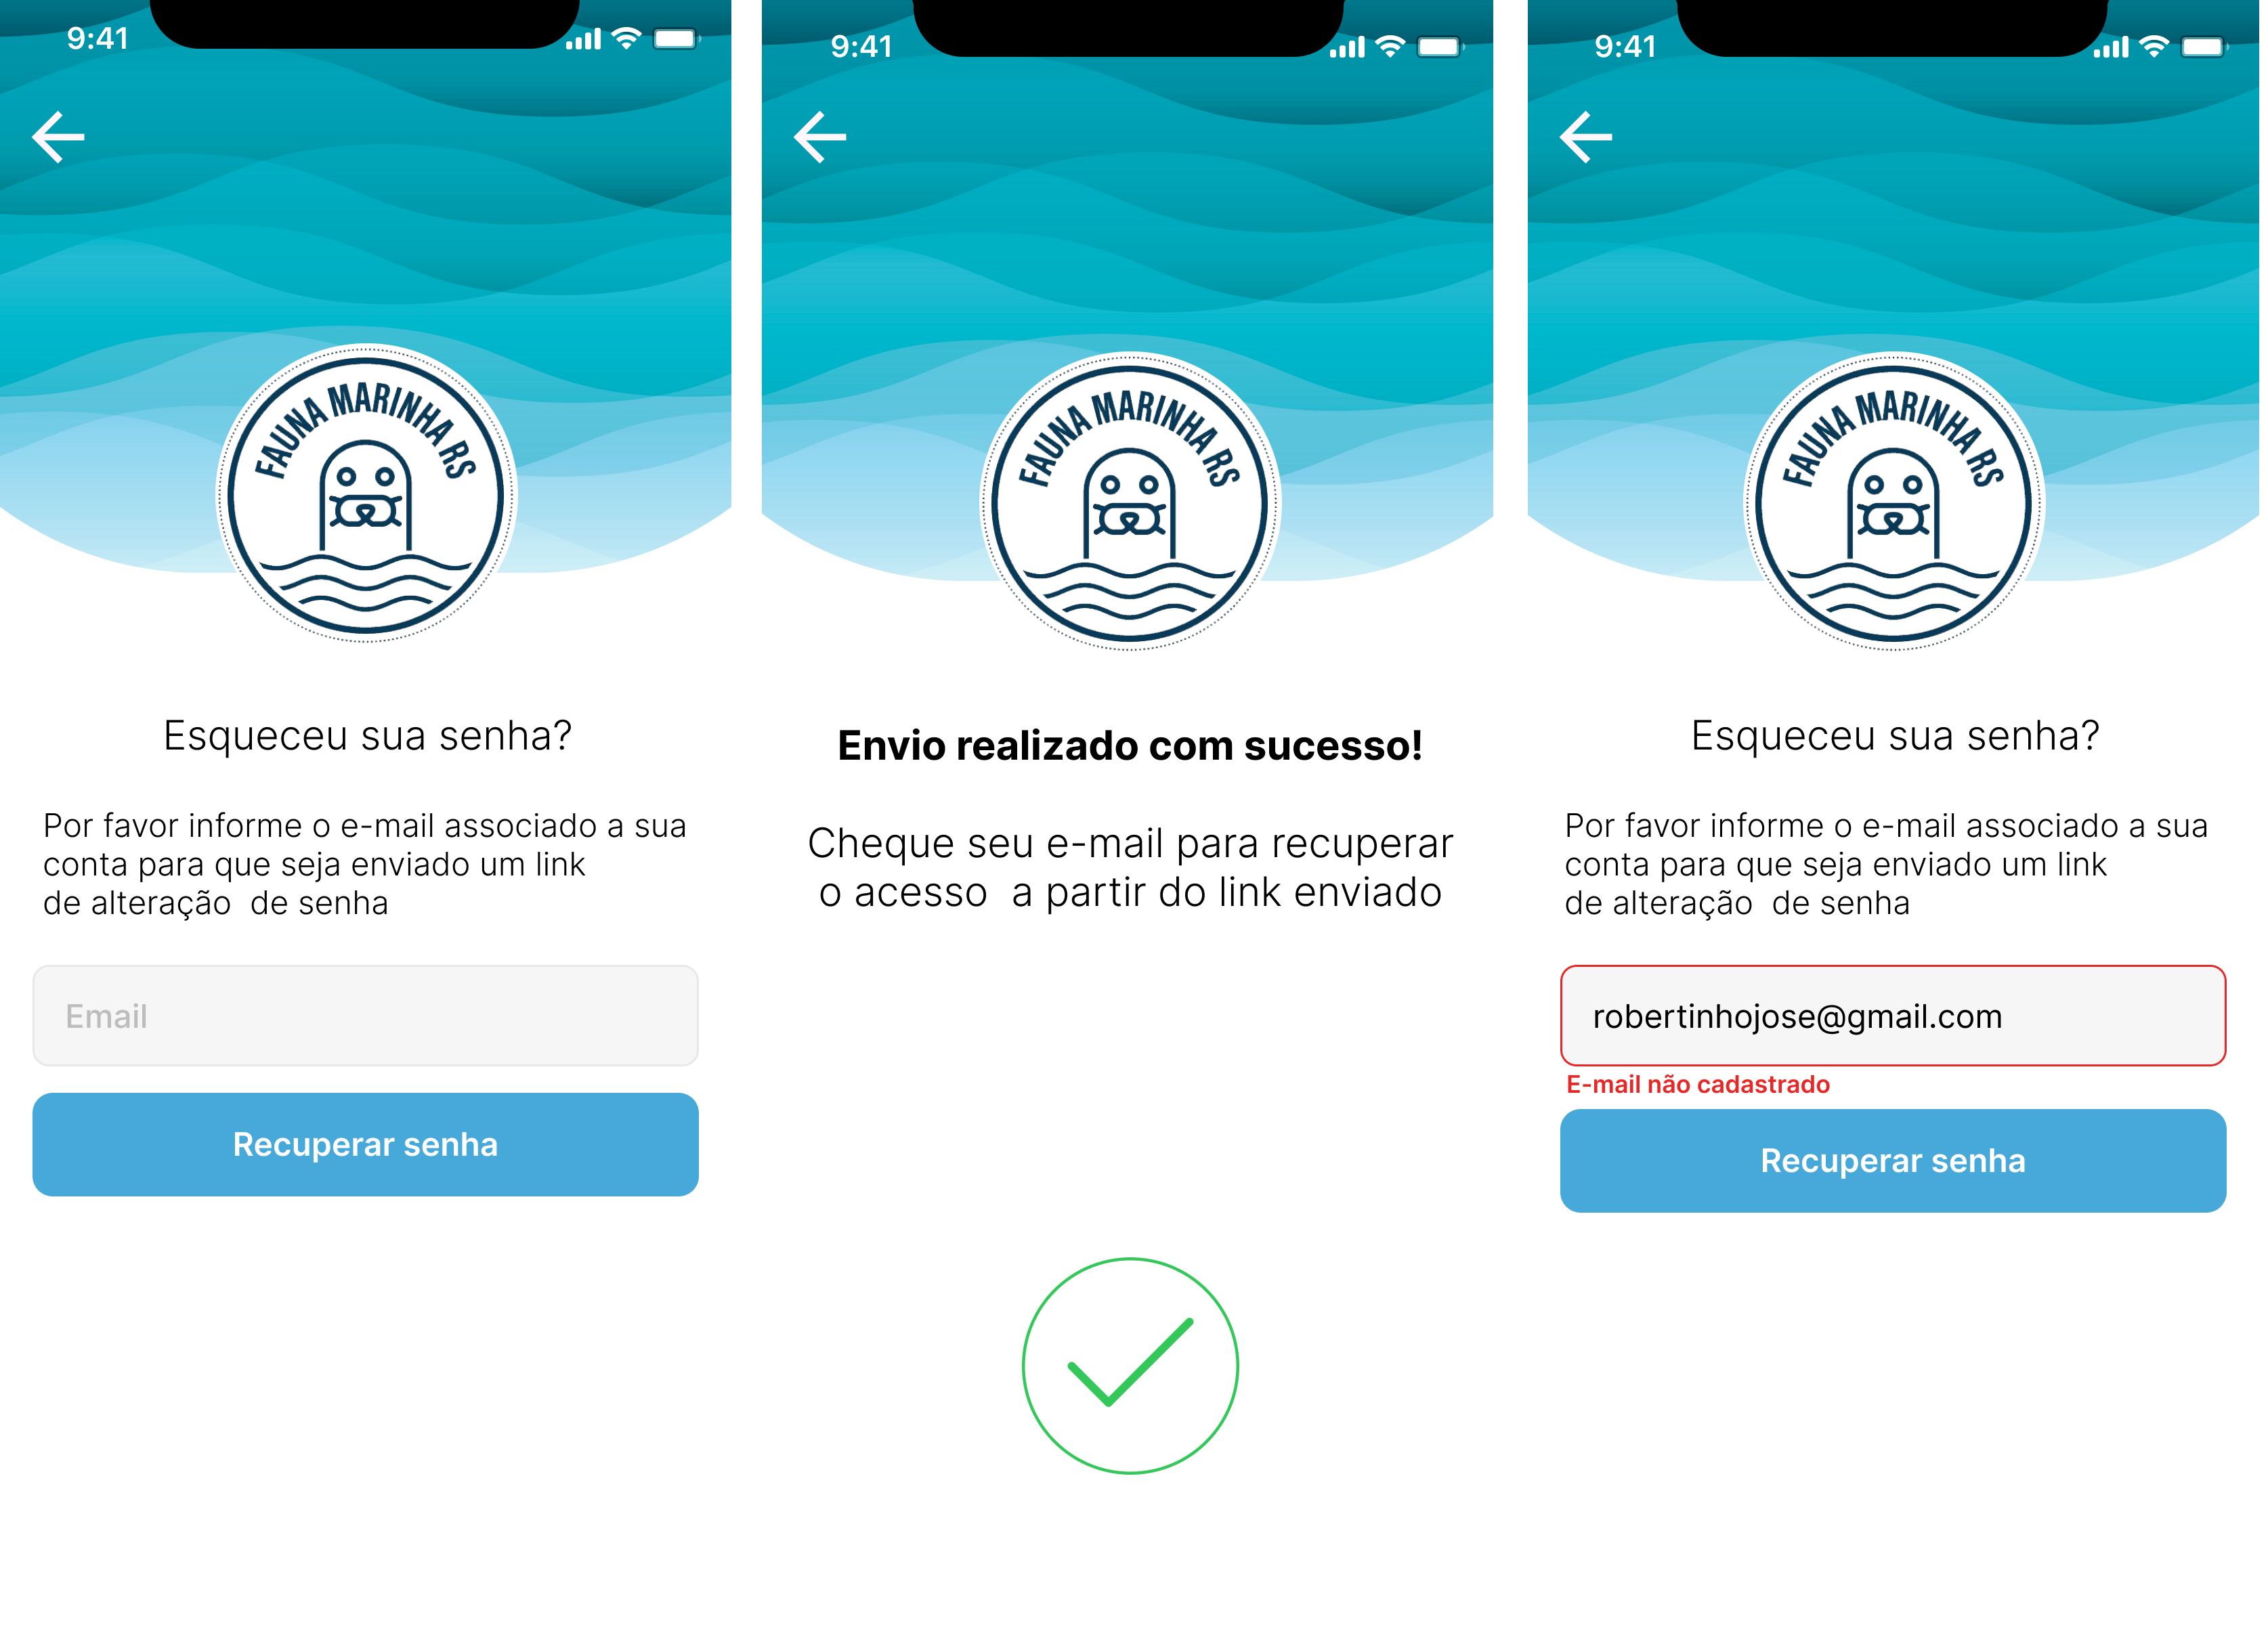
\includegraphics[height=0.53\textheight, width=\textwidth]{imagens/esqueceu-senha-figma.png}
    \caption{Protótipo da tela de recuperação de senha: formulário (esquerda), sucesso (centro) e erro de 
    validação (direita).}
    \label{fig:prototipo-esqueci-senha}
\end{figure}
\legend{Fonte: Autor}

\subsection{Desenvolvimento do Protótipo Navegável}

Utilizando a ferramenta \textit{Figma} (versão gratuita \textit{online}), foi desenvolvido um
protótipo navegável de média/alta fidelidade. Essa etapa permitiu visualizar os fluxos de 
interação entre o usuário e o sistema, antecipar ajustes necessários e alinhar as funcionalidades 
às expectativas.

Foram criadas ligações interativas entre as principais telas, simulando os redirecionamentos e 
ações de navegação. O protótipo também serviu como ferramenta de validação junto a terceiros e 
como referência visual para a fase de implementação (Figura~\ref{fig:prototipo-fluxo-navegacao}).

\begin{figure}[H]
    \centering
    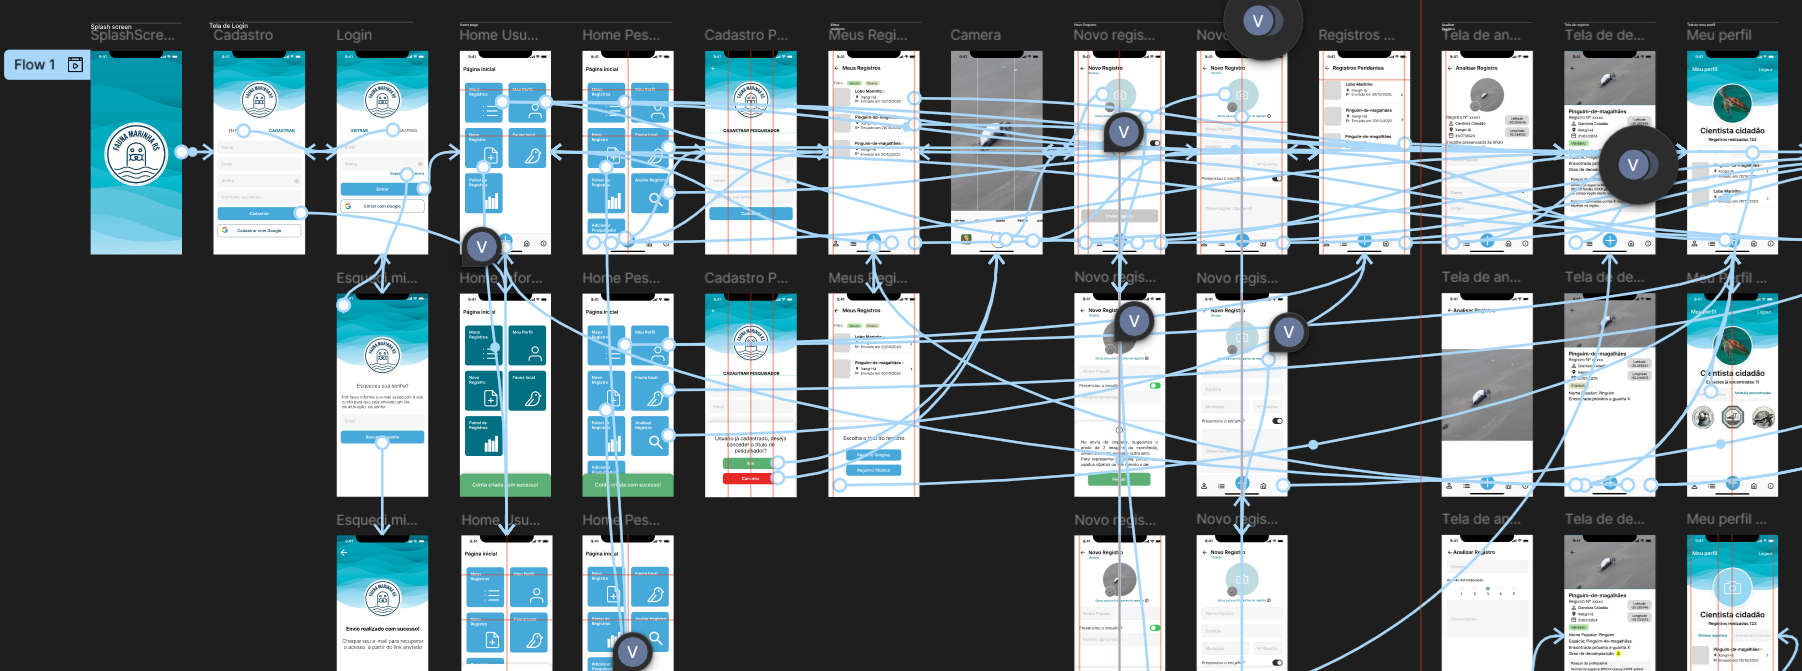
\includegraphics[width=\textwidth]{imagens/prototipo-navegavel-figma.png}
    \caption{Captura de tela do protótipo navegável desenvolvido no \textit{Figma}.}
    \label{fig:prototipo-fluxo-navegacao}
\end{figure}
\legend{Fonte: Autor}

\section{Projeto Gerencial}
% descrever o fluxo de trabalho documentado no Jira, com cards
A gerência desse projeto foi realizada utilizando a ferramenta \textit{Jira}, que possibilitou o
controle de tarefas e o acompanhamento do progresso do desenvolvimento. O fluxo de trabalho
descrito na \hyperref[sec:metodologia-desenv-software]{Seção de metodologia} deste trabalho foi 
seguido para garantir a organização e a eficiência
das tarefas. Os \textit{cards} gerados no \textit{board} foram puxados para trabalho a medida que 
havia tempo disponível para atuação. Foram catalogadas não só tarefas de codificação, como 
também tarefas de prototipação.

Foram gerados ao todo, 131 \textit{cards} desde julho de 2024 quando se deu inicio a prototipação 
da aplicação. Na Figura \ref{gra:cards-mes} é possível observar a quantidade de itens no eixo vertical
relacionada com o mês de criação no eixo horizontal. Com ele podemos concluir que os meses com 
mais entrada de demandas foram os meses de novembro de 2024, janeiro de 2025 e março de 2025,
onde o número de \textit{cards} criados foi maior que 18.

\begin{figure}[H]
    \centering
    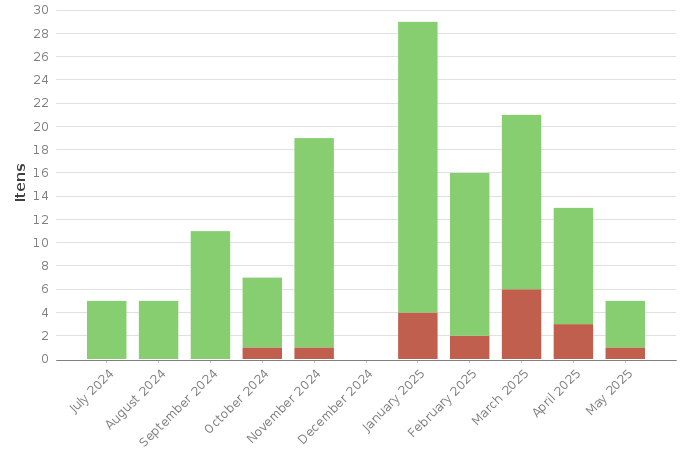
\includegraphics[width=\textwidth]{imagens/itensMes.png}
    \caption{Gráfico demonstrativo de \textit{cards} criados por mês no \textit{Jira}. As 
    barras em verde representam demandas que, até a data de criação do gráfico, já haviam sido finalizadas.
    As barras em vermelho representam demandas que ainda estavam em aberto.}
    \label{gra:cards-mes}
\end{figure}
\legend{Fonte: Autor}

A Figura \ref{gra:cards-vs-resolvidos} traz uma visão cumulativa do trabalho realizado no board.
A partir dele podemos ver que, dos 131 cards criados, 113 foram concluídos, o que representa 86,26\% 
do total. Podemos observar também que, em momentos de maior atuação no projeto, a criação de 
cards está diretamente relacionada com a quantidade de cards resolvidos.
Isso está principalmente relacionado com a disponibilidade de tempo para atuar no projeto, e também
com a criação de bugs e novas demandas que surgiram durante o desenvolvimento.

\begin{figure}[H]
    \centering
    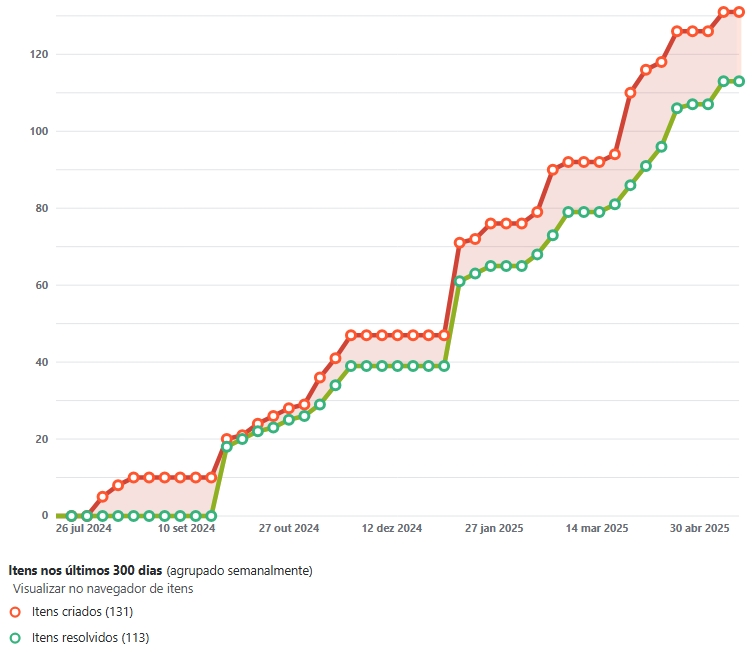
\includegraphics[width=\textwidth]{imagens/burnup-jira.jpeg}
    \caption{Gráfico demonstrativo de \textit{cards} vs resolvidos no \textit{Jira}}
    \label{gra:cards-vs-resolvidos}
\end{figure}
\legend{Fonte: Autor}

A Figura~\ref{gra:tempo-medio-resolucao} apresenta o tempo médio, em dias, 
para a resolução dos \textit{cards} ao longo das semanas. É possível notar uma grande variação 
nos tempos médios, com valores baixos no período de novembro e um pico em maio de 2025. 
Esse aumento progressivo reflete a falta de atuação evidenciada no mês de dezembro vide 
Figura\ref{gra:cards-vs-resolvidos}, o aumento na complexidade das demandas e o acumulo de 
cards de melhoria no \textit{Backlog} que foram criados e não priorizados.

\begin{figure}[H]
    \centering
    \includegraphics[width=\textwidth]{imagens/tempo-médio-cards.png}
    \caption{Gráfico demonstrativo de tempo de resolução médio dos \textit{cards} por semana no \textit{Jira}}
    \label{gra:tempo-medio-resolucao}
\end{figure}
\legend{Fonte: Autor}

Os \textit{cards} foram organizados em três grupos principais, que representam as diferentes
atuações necessárias para atuar em cada uma delas.
\subsection{Desenvolvimento Geral}
Esses cards representam demandas que passaram por etapas de planejamento e refinamento, 
refletindo as histórias de usuário e tarefas técnicas previstas ou requisitadas durante o desenvolvimento.
A Tabela~\ref{tab:desenv_geral_sorted} apresenta esse conjunto de funcionalidades. Ao todo foram 66 demandas
send 62 concluídas e 4 que ainda estão no \textit{Backlog}.

% manter essa tabela aqui ou colocar no anexo?
% talvez isso deveria ser um anexo? 

\begin{longtable}{@{}lp{7cm}ll@{}}
\caption{Registro de desenvolvimento geral (Ordenado por Data de Entrega)}\label{tab:desenv_geral_sorted}\\
\toprule
\textbf{Chave} & \textbf{Resumo} & \textbf{Status} & \textbf{Entregue} \\
\midrule
\endfirsthead

\caption{(Continuação) Registro de desenvolvimento geral (Ordenado por Data de Entrega)}\\
\toprule
\textbf{Chave} & \textbf{Resumo} & \textbf{Status} & \textbf{Entregue} \\
\midrule
\endhead

\midrule
\multicolumn{4}{r@{}}{(Continua na próxima página)} \\
\endfoot

\bottomrule
\endlastfoot

CEC-1 & Prototipação inicial das telas & Concluído & 2024-09-27 \\
CEC-2 & Tela de registro & Concluído & 2024-09-27 \\
CEC-3 & Tela de login & Concluído & 2024-09-27 \\
CEC-4 & Tela de novo registro Simples & Concluído & 2024-09-27 \\
CEC-5 & Tela de meus registros & Concluído & 2024-09-27 \\
CEC-6 & Tela de Coletanea animais & Concluído & 2024-09-27 \\
CEC-7 & Tela de perfil do usuário & Concluído & 2024-09-27 \\
CEC-8 & Tela de adicionar pesquisador & Concluído & 2024-09-27 \\
CEC-9 & Tela de esqueci minha senha & Concluído & 2024-09-27 \\
CEC-10 & Tela de selos de conquista & Concluído & 2024-09-27 \\
CEC-11 & Tela de novo registro Técnico & Concluído & 2024-09-27 \\
CEC-12 & Tela de home & Concluído & 2024-09-27 \\
CEC-13 & Tela de analisar Registro & Concluído & 2024-09-27 \\
CEC-14 & Tela de SplashScreen & Concluído & 2024-09-27 \\
CEC-15 & Tela sobre o app & Concluído & 2024-09-27 \\
CEC-16 & Codificação da SplashScreen & Concluído & 2024-09-27 \\
CEC-17 & Codificação da Tela de Registro & Concluído & 2024-09-28 \\
CEC-18 & Codificação da Tela de Login & Concluído & 2024-09-28 \\
CEC-21 & Codificação esqueci minha senha & Concluído & 2024-09-29 \\
CEC-20 & Codificação da Tela de Cadastrar Pesquisador & Concluído & 2024-10-03 \\
CEC-19 & Codificação da HomePage & Concluído & 2024-10-07 \\
CEC-22 & Adição funcionalidade de adicionar novo registro + bottom sheet & Concluído & 2024-10-09 \\
CEC-23 & Tela de registro simples & Concluído & 2024-10-15 \\
CEC-24 & Tela de registro tecnico & Concluído & 2024-10-21 \\
CEC-25 & Tela de registro controller & Concluído & 2024-10-21 \\
CEC-28 & Tela de perfil do usuário & Concluído & 2024-11-02 \\
CEC-30 & Mensagens de feedback para usuario: sucesso e erro & Concluído & 2024-11-23 \\ 
CEC-29 & Tela Meus registros & Concluído & 2024-11-03 \\
CEC-31 & Criar listas para os itens da tela de perfil & Concluído & 2024-11-03 \\
CEC-33 & Tela view de Registro & Concluído & 2024-11-08 \\
CEC-35 & Texto da tela de sobre o app & Concluído & 2024-11-16 \\
CEC-38 & Adicionar dependencia e configurar para captar a localizacao & Concluído & 2024-11-10 \\
CEC-34 & Criar montagem do registro + cadastrar registro & Concluído & 2024-11-11 \\
CEC-40 & Tela de avaliar registro & Concluído & 2024-11-15 \\
CEC-39 & Adicionar botao para remover imagem adicionada & Concluído & 2024-11-16 \\ 
CEC-42 & Funcionalidade de deletar conta & Concluído & 2024-11-23 \\
CEC-44 & Tratamento de erros do login firebase & Concluído & 2024-11-23 \\ 
CEC-41 & Adicionar badge para o icone de meus registros & Concluído & 2024-11-23 \\ 
CEC-48 & Criação do BD firebase & Concluído & 2025-01-07 \\
CEC-53 & Ordenaçao por data dos registros & Concluído & 2025-01-08 \\
CEC-59 & Adicionar skeleton de carregamento em alguns widgets & Concluído & 2025-01-09 \\
CEC-46 & Lógica de adição de pesquisador + lógica de conceder role de pesquisador pra usuário já existente & Concluído & 2025-01-10 \\
CEC-66 & Adição de uma badge para avisar registros nao visualizados & Concluído & 2025-01-11 \\
CEC-60 & Adicionar facilidade para ativar a geolocalizacao do dispositivo & Concluído & 2025-01-11 \\
CEC-78 & Skeletonizer tela inicial & Concluído & 2025-02-14 \\
CEC-98 & Geração de csv para exportação & Concluído & 2025-03-21 \\
CEC-54 & Tela painel de registros & Concluído & 2025-03-23 \\
CEC-110 & Adicionar update de localização na avaliação do registro & Concluído & 2025-03-31 \\
CEC-116 & Atualização da versão do projeto* & Concluído & 2025-03-31 \\
CEC-111 & Adicionar o campo das quaritas/ municipio para avaliar registro & Concluído & 2025-03-31 \\
CEC-118 & Adição de campo livre ponto de referencia & Concluído & 2025-04-06 \\
CEC-112 & Migraçao dos dados atuais para o firebase & Refinamento & 2025-04-06 \\
CEC-109 & Deletar registros & Concluído & 2025-04-07 \\
CEC-125 & badges para classes no perfil com contador & Concluído & 2025-04-17 \\
CEC-106 & Possibilidade de adicionar um novo animal nao presente no banco de dados quando for identificado & Concluído & 2025-04-18 \\
CEC-114 & Modificar restrições do csv & Concluído & 2025-04-18 \\
CEC-108 & Filtrar quantidade por classe & Concluído & 2025-04-18 \\
CEC-55 & Criação de badges para os animais & Concluído & 2025-04-23 \\
CEC-49 & Implementar cache dos registros enviados quando nao há internet & Concluído & 2025-05-12 \\
CEC-37 & Realizar integração front para receber dados da API baseado em criterios dos inputs & Concluído & 2025-05-12 \\
CEC-76 & Ajustes de responsividade devices menors & Concluído & 2025-05-12 \\
CEC-107 & Adicionar pedido para que a pessoa nao mostre seu rosto no informativo da foto & Concluído & 2025-05-12 \\
CEC-81 & Desenvolvimento de redirect para opção de fauna local & Concluído & 2025-05-12 \\
CEC-58 & Tela fauna local & Backlog & \\
CEC-115 & Gerar termos de uso & Backlog & \\
CEC-105 & Adicionar campo de tipo de usuário que realizou o envio do registro & Backlog & \\
CEC-113 & Mapa para marcar local aproximado no envio do registro & Backlog & \\

\end{longtable}

\subsection{Correções}
Ao longo do processo de desenvolvimento, foram identificados e registrados bugs e falhas 
de funcionamento, a origem da geração desses cards pode ser tanto de testes internos, quanto de 
validações de testadores que obtiveram alguma das builds do projeto e reportaram alguma inconsistência. 
Essas inconsistências foram tratadas por meio de cards como correções (\textit{fixes}) no ambiente Jira.

A Tabela~\ref{tab:fixes_sorted} a seguir apresenta uma relação dos 43 apontamentos dessa categoria que foram documentados, desse total, 
42 foram resolvidos e 1 ainda está no \textit{Backlog}. Isso demonstra a evolução contínua do 
sistema em busca de estabilidade e qualidade do produto final.

% manter essa tabela aqui ou colocar no anexo?

\begin{longtable}{@{}lp{7cm}ll@{}}
\caption{Registro de Correções (Fixes) (Ordenado por Data de Entrega)}\label{tab:fixes_sorted}\\
\toprule
\textbf{Chave} & \textbf{Resumo} & \textbf{Status} & \textbf{Entregue} \\
\midrule
\endfirsthead

\caption{(Continuação) Registro de Correções (Fixes) (Ordenado por Data de Entrega)}\\
\toprule
\textbf{Chave} & \textbf{Resumo} & \textbf{Status} & \textbf{Entregue} \\
\midrule
\endhead

\midrule
\multicolumn{4}{r@{}}{(Continua na próxima página)} \\
\endfoot

\bottomrule
\endlastfoot

CEC-61 & Fix: Feedback para o usuario quando um registro offline é enviado & Concluído & 2025-01-10 \\
CEC-67 & Fix: Ajustes de condicionais de tela de avaliar registro & Concluído & 2025-01-11 \\
CEC-65 & Fix: Mensagem de não adição de imagem & Concluído & 2025-01-11 \\
CEC-69 & Fix: Ajuste de envio da imagem independente do input escolhido & Concluído & 2025-01-11 \\
CEC-63 & Fix: Adicionar um icone X no input de dropdown para deletar o conteudo & Concluído & 2025-01-11 \\
CEC-36 & Fix: Mensagem de dicas para fotografia & Concluído & 2025-01-11 \\
CEC-71 & Fix: Deletar foto de perfil quando conta é deletada & Concluído & 2025-01-11 \\
CEC-62 & Fix: Ajustar visualização de filtros para ser mais intuitivo & Concluído & 2025-01-11 \\
CEC-56 & Fix: Ajuste do header registros pendentes + meus registros & Concluído & 2025-01-17 \\
CEC-77 & Fix: Ajuste dos cards de meus registros (responsividade) & Concluído & 2025-01-23 \\
CEC-92 & Fix: Ajuste de italico na apresentação da taxonomia & Concluído & 2025-02-22 \\
CEC-95 & Fix: Alterar a quantidade de caracteres do campo obs para 600 + travar escrita & Concluído & 2025-02-22 \\
CEC-83 & Fix: Ajuste no regex de cadastro do campo de nome popular & Concluído & 2025-02-22 \\
CEC-94 & Fix: Ajuste de campos opcionais que estao sendo apresentados como obrigatorios no envio da avaliacao do registro & Concluído & 2025-02-22 \\
CEC-88 & Fix: A partir da localizacao do registro adicionar o campo nome da cidade & Concluído & 2025-02-23 \\
CEC-90 & Fix: Na tela de registro simples, permitir que o usuario adicione a cidade e a guarita & Concluído & 2025-02-23 \\
CEC-86 & Fix: Alteração do gráfico em pontos por gráfico em barras tela de painel de registros & Concluído & 2025-02-23 \\
CEC-99 & Fix: Campo de obs nao está sendo mantido & Concluído & 2025-03-21 \\
CEC-102 & Fix: Botão voltar tela de registros avaliados & Concluído & 2025-03-23 \\
CEC-100 & Fix: Loading da image do bottomsheet mapa & Concluído & 2025-03-24 \\
CEC-117 & Fix: Limpar dados de guarita municipio & Concluído & 2025-04-01 \\
CEC-119 & Fix: Ajustar aparecimento dos botoes de avaliar registro + adicionar pesquisador & Concluído & 2025-04-05 \\
CEC-121 & Fix: Validaçao de liberar envio de registros & Concluído & 2025-04-06 \\
CEC-101 & Fix: Loading entrar com Google ausente & Concluído & 2025-04-06 \\
CEC-127 & Fix: Ajuste na visualizacao do retorno do profissional na tela de register view & Concluído & 2025-04-17 \\
CEC-126 & Fix: Ajuste de estado inicia do seletor dde avaliar registro & Concluído & 2025-04-17 \\
CEC-128 & Fix: Classe no model de AnimalResponse & Concluído & 2025-04-18 \\
CEC-131 & Fix: Overflow do nome na tela de perfil & Concluído & 2025-04-18 \\
CEC-132 & Fix: Problema no envio de registro offline sem localização & Concluído & 2025-05-06 \\
CEC-133 & Fix: Validacao dos campos registros simples & Concluído & 2025-05-06 \\
CEC-134 & Fix: Ajuste de mostrar registros de guaritdas no mapa & Concluído & 2025-05-06 \\
CEC-136 & Fix: Formatacao de coordenadas quando randomizador de guarita é acionadio & Concluído & 2025-05-06 \\
CEC-43 & Fix: Arrumar redirect após o cadastro & Concluído & 2025-05-12 \\
CEC-50 & Fix: Alteração semantica do campo de genero & Concluído & 2025-05-12 \\
CEC-51 & Fix: Ajustes propostos pela professora Karen & Concluído & 2025-05-12 \\
CEC-52 & Fix: Comportamento do dropdown dos inputs de pesquisa & Concluído & 2025-05-12 \\
CEC-68 & Fix: Ajustes de condicionais da tela de visualizar registro & Concluído & 2025-05-12 \\
CEC-75 & Fix: Adicionar lógica de contador de animais encontrados após avaliações & Concluído & 2025-05-12 \\
CEC-79 & Fix: Lógica para permitir acesso a features offline HomePage & Concluído & 2025-05-12 \\
CEC-130 & Fix: Ajuste de bloqueio de switch quando gps esta desligado & Concluído & 2025-05-12 \\
CEC-82 & Fix: Ajuste no datePicker register pannel & Concluído & 2025-05-12 \\
CEC-85 & Fix: Ajuste no tamanho do campo de observacao e retorno do profissional & Concluído & 2025-05-12 \\
CEC-80 & Fix: Enviar e manipular o switch permite duplicar o registro & Concluído & 2025-05-12 \\
CEC-104 & Fix: Campo de busca quando apagado deve apresentar todas as opcoes novamente & Backlog & \\

\end{longtable}


\subsection{Débitos Técnicos e Melhorias}
Além das funcionalidades previstas e dos \textit{bugs} encontrados, também foram abertos \textit{cards} 
para apontamentos de melhorias para algumas funcionalidades e respostas do sistema e débitos técnicos produzidos 
durante a codificação. 
Esses pontos surgiram durante a implementação de funcionalidades, revisões de código ou testes 
exploratórios e regressivos.

A Tabela~\ref{tab:dt_melhorias_sorted} apresenta as melhorias e ajustes técnicos catalogados, 
evidenciando práticas de refatoração e aprimoramento contínuo. Ao todo foram 19 \textit{cards} abertos com esse intuito,
dos quais 8 foram resolvidos e 11 ainda estão no \textit{Backlog}.

% manter essa tabela aqui ou colocar no anexo?
% talvez isso deveria ser um anexo? 
\begin{longtable}{@{}lp{7cm}ll@{}}
\caption{Registro de Débitos Técnicos e Melhorias (Ordenado por Data de Entrega)}\label{tab:dt_melhorias_sorted}\\
\toprule
\textbf{Chave} & \textbf{Resumo} & \textbf{Status} & \textbf{Entregue} \\
\midrule
\endfirsthead

\caption{(Continuação) Registro de Débitos Técnicos e Melhorias (Ordenado por Data de Entrega)}\\
\toprule
\textbf{Chave} & \textbf{Resumo} & \textbf{Status} & \textbf{Entregue} \\
\midrule
\endhead

\midrule
\multicolumn{4}{r@{}}{(Continua na próxima página)} \\
\endfoot

\bottomrule
\endlastfoot
CEC-74 & Melhoria: Adicionar um marcador nos registros que ainda nao foram visualizados na tela de meus registros & Concluído & 2024-11-23\\
CEC-73 & Melhoria: Poder abrir a imagem na tela de visualizar registro & Concluído & 2025-01-11 \\
CEC-70 & Melhoria: Melhorar carregamento das imagens nas telas que apresentam todos os registros & Concluído & 2025-01-11 \\
CEC-123 & Melhoria: Alterar nome de salvamento das imagens dos registros & Concluído & 2025-04-07 \\
CEC-129 & Melhoria Adicionar loading no botao de avaliar registro & Concluído & 2025-04-18 \\
CEC-87 & Melhoria: Captar localizacao de uma imagem da galeria quando presente & Concluído & 2025-05-12 \\
CEC-32 & Melhoria: Ajustar centralização da lista de badges na tela de perfil & Concluído & 2025-05-12 \\
CEC-96 & Melhoria: Adicionar switch para envio de imagens da galeria tela de registro técnico & Concluído & 2025-05-12 \\
CEC-93 & Melhoria: Adicionar pré cadastro dos municpios do litoral norte, apenas seleção & Concluído & 2025-05-12 \\
CEC-45 & Melhoria: Modificar logica de tratamento de exceptions para remocao da passagem de BuildContext & Backlog &  \\
CEC-124 & Melhoria: Notificação quando registro é avaliado & Backlog & \\
CEC-122 & Melhoria: Exception de email nao encontrado & Backlog & \\
CEC-137 & Melhoria: Lógica de retry quando a internet está ruim & Backlog & \\
CEC-91 & Melhoria: Glossário ilustrado dos principais animais & Backlog & \\
CEC-57 & Melhoria: Validação de email cadastrado esqueci minha senha & Backlog & \\
CEC-120 & Melhoria: Criar uma thumb com a imagem dos registros no mapa do painel & Backlog & \\
CEC-26 & Melhoria: Refac da navegação & Backlog & \\
CEC-97 & Fix: Alteracao da ordem dos campos do formulário de avaliar registro & Backlog & \\
CEC-72 & Fix: Ajustar lógica de visualização da foto de perfil & Backlog & \\
CEC-103 & Fix: Pop up informando saída do app no botao de fauna local & Backlog & \\

\end{longtable}



\section{Implementação do Sistema}
% descrever a implementação do sistema, com detalhes técnicos e decisões de projeto.
% incluir imagens de telas, fluxos de navegação, etc.
% fazer relações com o projeto gerencial e com os requisitos funcionais e não funcionais.

\subsection{Banco de Dados}
\begin{table}[H]
    \centering
    \caption{Estrutura de collections do banco de dados}
    \label{tab:estrutura-dados}
    \begin{tabular}{|p{3cm}|p{10cm}|}
    \hline
    \textbf{Collection} & \textbf{Descrição} \\ \hline
    \texttt{counters} & Armazena contadores gerais (ex.: número total de animais cadastrados e registros realizados). \\ \hline
    \texttt{animals} & Armazena todas as espécies já registradas no sistema, com dados taxonômicos completos. \\ \hline
    \texttt{users} & Armazena informações dos usuários. Cada usuário contém uma subcollection \texttt{registers} com seus registros individuais. \\ \hline
    \end{tabular}
\end{table}
\legend{Fonte: Autor}

\section{Execução de Testes e Verificação de Qualidade}

% Descrever testes, citar testadores, resultados dos testes e estratégias futuras.
% incluir gráficos representativos trazendo resultados dos testes e relacionar com 
% cards gerados para o Jira

\section*{Considerações Finais}

O capítulo consolidou os resultados até aqui obtidos, alinhando-os ao planejamento inicial do projeto, garantindo rastreabilidade entre requisitos, projeto e implementação.

% ---

% ---
% Conclusão
% ---
\chapter{Conclusão}
% ---

\lipsum[31-33]
% ---

% ----------------------------------------------------------
% ELEMENTOS PÓS-TEXTUAIS
% ----------------------------------------------------------
\postextual
% ----------------------------------------------------------

% ----------------------------------------------------------
% Referências bibliográficas (Obrigatório)
% ----------------------------------------------------------
\bibliography{elementos-pos-textuais/referencias}


% ----------------------------------------------------------
% Glossário (Opcional)
% ----------------------------------------------------------
%
% Consulte o manual da classe abntex2 para orientações sobre o glossário.
%
%\glossary


% ----------------------------------------------------------
% Apêndices (Opcional)
% ----------------------------------------------------------
% ---
% Inicia os apêndices
% ---
\begin{apendicesenv}

% ----------------------------------------------------------
\chapter{Quisque libero justo}
% ----------------------------------------------------------

\lipsum[50]
% ----------------------------------------------------------
\chapter{Nullam elementum urna vel imperdiet sodales elit ipsum pharetra ligula
ac pretium ante justo a nulla curabitur tristique arcu eu metus}
% ----------------------------------------------------------
\lipsum[55-57]

\end{apendicesenv}
% ---


% ----------------------------------------------------------
% Anexos (Opcional)
% ----------------------------------------------------------
% ---
% Inicia os anexos
% ---
\begin{anexosenv}

% ---
\chapter{Morbi ultrices rutrum lorem.}
% ---
\lipsum[30]
% ---
\chapter{Cras non urna sed feugiat cum sociis natoque penatibus et magnis dis
parturient montes nascetur ridiculus mus}
% ---

\lipsum[31]
% ---
\chapter{Fusce facilisis lacinia dui}
% ---

\lipsum[32]

\end{anexosenv}


%---------------------------------------------------------------------
% INDICE REMISSIVO (Opcional)
%---------------------------------------------------------------------
%\phantompart
%\printindex
%---------------------------------------------------------------------

\end{document}
